\documentclass[10pt,aspectratio=43,unknownkeysallowed]{beamer}

\usepackage{xcolor}
\usepackage{amsmath,amsfonts,amsthm,amssymb}
\usepackage{graphicx}


\newcommand{\srcimages}{srcimages}           % Source images dir. name
\newcommand{\images}{images}                 % create images dir. name
\newcommand{\prebuiltimages}{prebuiltimages} % prebuiltimages images dir. name

\graphicspath{{../\images}}
\usepackage[rotationcw]{beamer_sty}% clockwise, default is counterclockwise

\usepackage[utf8]{inputenc}
\usepackage[english]{babel}
\usepackage[T1]{fontenc}
\usepackage{copyrightbox}
\usepackage{hyperref}
\usepackage{cleveref}
\usepackage[inline]{enumitem}
% \setlist[itemize]{itemjoin=\hspace*{\fill},itemjoin*=\hspace*{\fill}}
\setlist[itemize]{label=$\blacktriangleright$}

\usepackage[scaled]{beramono}
\usepackage[scale=1.05]{AlegreyaSans}
\usepackage{caption}
\usepackage{subcaption}
\usepackage{booktabs} % for professional tables
\usepackage{minted}
\usepackage{mathtools}
\usepackage{bbm}
\usepackage{wrapfig}
\usepackage[export]{adjustbox}
\usepackage{csquotes}
\usepackage{dsfont}

% for tikz
\usepackage[titlenumbered,ruled,linesnumbered,noend]{algorithm2e}

\usepackage{tikz}
%\usetikzlibrary{trees}
\usetikzlibrary{arrows,shapes,positioning,shadows,trees,mindmap}
% \usepackage{forest}
\usepackage[edges]{forest}
\usetikzlibrary{arrows.meta}
\colorlet{linecol}{black!75}
\usepackage{xkcdcolors} % xkcd colors


% for colorful equation
\usetikzlibrary{backgrounds}
\usetikzlibrary{arrows,shapes}
\usetikzlibrary{tikzmark}
\usetikzlibrary{calc}
% Commands for Highlighting text -- non tikz method
\newcommand{\highlight}[2]{\colorbox{#1!17}{$\displaystyle #2$}}
%\newcommand{\highlight}[2]{\colorbox{#1!17}{$#2$}}
\newcommand{\highlightdark}[2]{\colorbox{#1!47}{$\displaystyle #2$}}

% Commands for Highlighting text -- non tikz method
\renewcommand{\highlight}[2]{\colorbox{#1!17}{#2}}
\renewcommand{\highlightdark}[2]{\colorbox{#1!47}{#2}}

%\usepackage{minted}
\usepackage{tkz-fct}
% \pgfplotsset{compat=1.17}
%\usetikzlibrary{spy}
% \usepackage[round]{natbib}
% \bibliographystyle{plainnat}
\addbibresource{../biblio.bib}

\DeclarePairedDelimiter{\abs}{\lvert}{\rvert}
\usepackage{dsfont}
\newcommand{\ind}{\mathds{1}}
\def\1{\mathbf 1}

\definecolor{javared}{rgb}{0.6,0,0} % for strings
\definecolor{javagreen}{rgb}{0.25,0.5,0.35} % comments
\definecolor{javapurple}{rgb}{0.5,0,0.35} % keywords
\definecolor{javadocblue}{rgb}{0.25,0.35,0.75} % javadoc
\definecolor{marron}{rgb}{0.64,0.16,0.16}
\definecolor{orange_js}{RGB}{230,159,0}
\colorlet{LightGray}{gray!40}
\definecolor{chocolate}{rgb}{0.48, 0.25, 0.0}
\definecolor{deepmagenta}{rgb}{0.8, 0.0, 0.8}
\newcommand{\mybold}[1]{\textcolor{marron}{\textbf{#1}}}
\newcommand{\cRm}[1]{\textsc{\romannumeral #1}}
\newcommand{\inred}[1]{\textcolor{red}{#1}}
\usetikzlibrary{decorations.pathmorphing}
\definecolor{paper}{RGB}{211,211,211}

\usepackage{xspace}
\newcommand{\ie}{{\em{i.e.,}}\xspace}
\newcommand{\etal}{{\em{et al.}}\xspace}
\newcommand{\eg}{{\em{e.g.,}}\xspace}
\newcommand{\lcf}{{\em cf.~}}
\newcommand{\st}{{{s.t.}}\xspace}
\newcommand{\iid}{{\em{i.i.d.}}\xspace}
\newcommand{\VA}{{\em v.a. {}}}
\newcommand{\rem}{\underline{Rem}:~}
\newcommand{\wrt}{with respect to\xspace}
\newcommand{\ow}{o.w.\xspace}

\usepackage{pifont}%
\newcommand{\xmark}{\ding{55}}%
\newcommand{\cmark}{\ding{51}}%
\def\scalecheck{\resizebox{\widthof{\cmark}*\ratio{\widthof{x}}{\widthof{\normalsize x}}}{!}{\cmark}}
\def\scalecross{\resizebox{\widthof{\xmark}*\ratio{\widthof{x}}{\widthof{\normalsize x}}}{!}{\xmark}}

% allow pauses in align
\makeatletter
\let\save@measuring@true\measuring@true
\def\measuring@true{%
  \save@measuring@true
  \def\beamer@sortzero##1{\beamer@ifnextcharospec{\beamer@sortzeroread{##1}}{}}%
  \def\beamer@sortzeroread##1<##2>{}%)
  \def\beamer@finalnospec{}%
}
\makeatother


%%%%%%%%%%%%%%%%%%%%%%%%%%%%%%%%%%%%%%%%%%%%%%%%%%%%%%%%%%%%%%%%%%%%%%%%%%%%%%%
%%%%%%%%%%%%%%%%%%%%%%%%%%%%%%%%%%%%%%%%%%%%%%%%%%%%%%%%%%%%%%%%%%%%%%%%%%%%%%%
% HEADER
%%%%%%%%%%%%%%%%%%%%%%%%%%%%%%%%%%%%%%%%%%%%%%%%%%%%%%%%%%%%%%%%%%%%%%%%%%%%%%%
%%%%%%%%%%%%%%%%%%%%%%%%%%%%%%%%%%%%%%%%%%%%%%%%%%%%%%%%%%%%%%%%%%%%%%%%%%%%%%%

\title[] %shown at the top of frames
{
    Label ambiguity in crowdsourcing \\ for classification and
    expert feedback} %shown in title frame

\date{09-20-2024} % explicitly set date- Le parc zoologique est ouvert.
\author[]%shown at the top of frames
{%shown in title frame
    {\textbf{Tanguy Lefort}\\ IMAG, Univ Montpellier, CNRS \\ INRIA, LIRMM,}%
    \vspace{1cm}\\
    {Supervised by\\ \hspace{.5cm} \textbf{Benjamin Charlier} \\ \hspace{.5cm}\textbf{Alexis Joly} \\ \hspace{.5cm} and \textbf{Joseph Salmon}}%
}
\institute[
]
{% is placed on the bottom of the title page
}

\titlegraphic{% logos are put at the bottom-right part of the page
    % \includesvgpdf{All_logos}{width=5cm} % logo
    
\includegraphics[width=5cm]{../images/All_logos_new.pdf}% up to 3 (after it gets messy)
    % \includegraphics[width=2cm]{CNRS.pdf} % if more, combine them in one image.
    % \includegraphics[width=2cm]{inr_logo_rouge_cmjn.pdf} % if more, combine them in one image.
    }

\setbeamercolor{itemize subitem}{fg=javadocblue}
\setbeamertemplate{itemize subitem}[triangle]
\setbeamercolor{subsection in toc}{fg=black}

\def\Put(#1,#2)#3{\leavevmode\makebox(0,0){\put(#1,#2){#3}}}

\begin{document}
\maketitle
% \section{Intro}

\begin{frame}{How to train your classifier}{}

\foreach \i in {1,...,6} {
    \begin{onlyenv}<\i>
        \includegraphics[width=\textwidth]{./images/questioning_labels_\i.pdf}
    \end{onlyenv}
}
\end{frame}

\begin{frame}{Ask citizens to label our data}{Framework and notations}
    \begin{itemize}
        \item Workers sort a given task into one of the $K$ classes
    \end{itemize}
\visible<1-2>{
   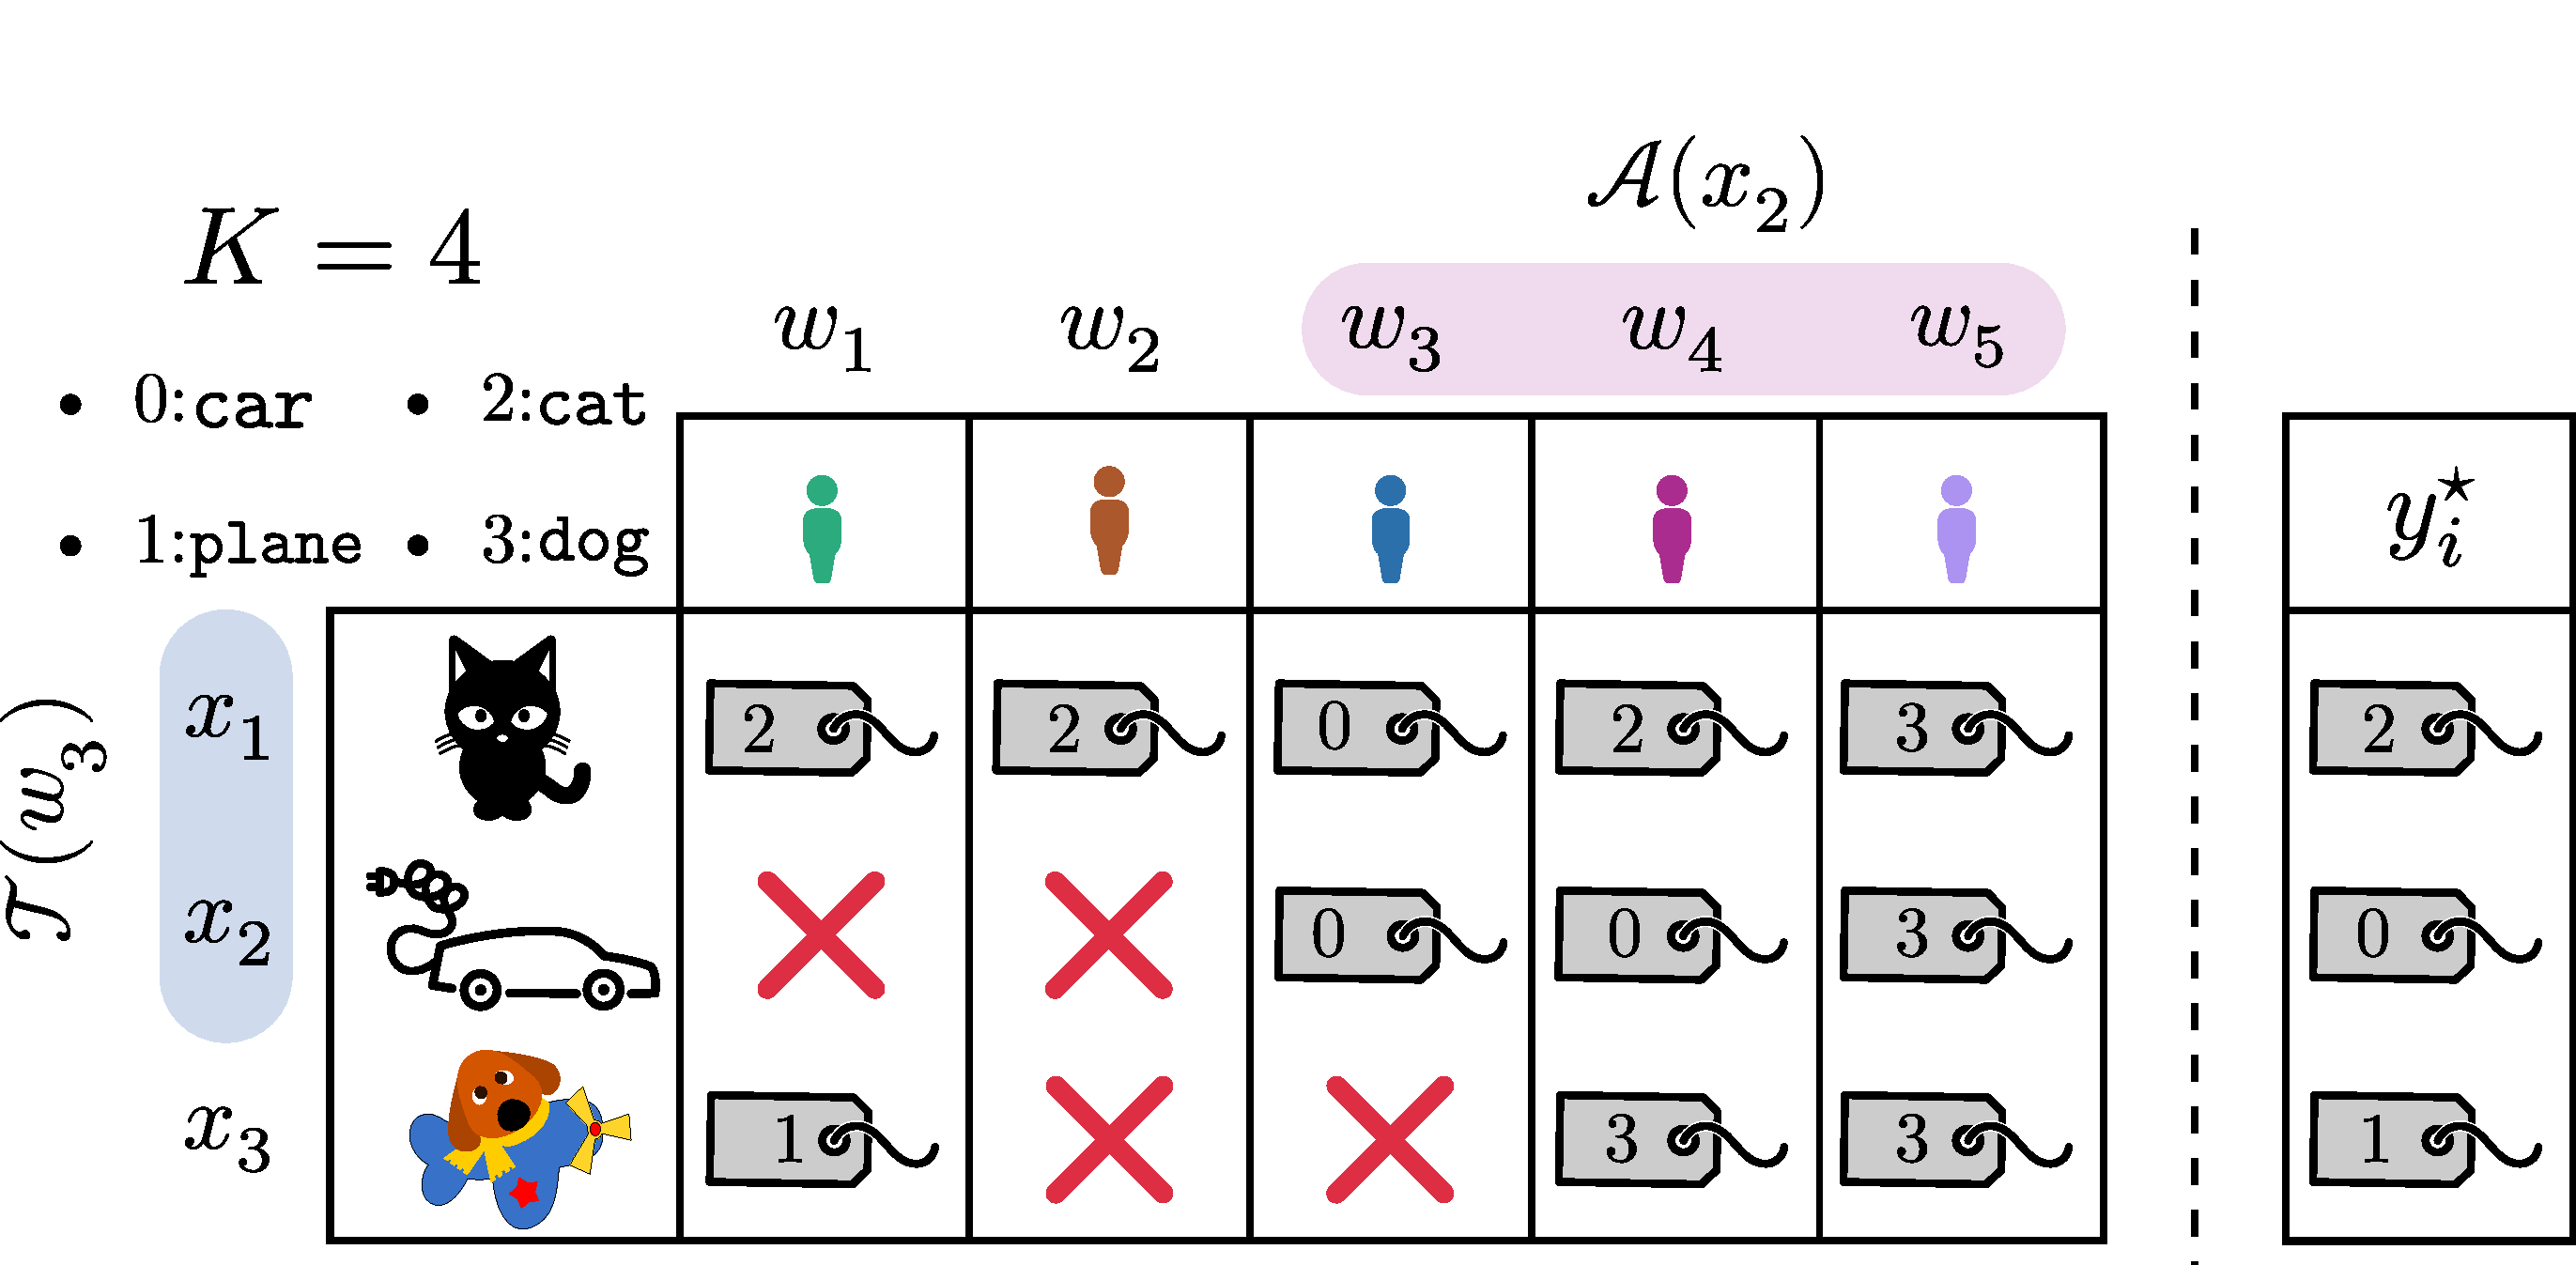
\includegraphics[width=\textwidth, clip,trim={0cm 4cm 0cm 0cm}]{./images/notations_1.pdf}
}%
\visible<2->{
\begin{itemize}
    \item $ y_i^{(j)}\in [K]:= \text{ answer of worker } j \text{ to task }i$
    \item $n_{\text{worker}}$ workers answer $n_{\text{task}}$ tasks
\end{itemize}
}
\end{frame}

%%%%%%%%%%%%%%%%%%%%%%%%%%%%%%%%%%%%%%%%%%%%%%%%%%%%%%%%%%%%%%%%%%%%%%%%%%%%%%%
\begin{frame}{From the data to the classifier}{The pipeline}
    \foreach \i in {1,...,5} {
        \begin{onlyenv}<\i>
            \includegraphics[width=\textwidth]{./images/strategies_crowd_data_\i.pdf}
        \end{onlyenv}
    }
    \end{frame}
%%%%%%%%%%%%%%%%%%%%%%%%%%%%%%%%%%%%%%%%%%%%%%%%%%%%%%%%%%%%%%%%%%%%%%%%%%%%%%%

%%%%%%%%%%%%%%%%%%%%%%%%%%%%%%%%%%%%%%%%%%%%%%%%%%%%%%%%%%%%%%%%%%%%%%%%%%%%%%%
\begin{frame}{Main contributions}{}

\begin{itemize}[itemsep=20pt]
    \item<1-> Can we improve performance by leveraging better-quality data?
    \begin{itemize}
        \item<4-> Creation of the \textbf{WAUM}\footfullcite{lefort2022improve}: a metric to identify ambiguous images %
    \end{itemize}
    \item<2-> Can we standardize crowdsourcing dataset's tools in \texttt{python} for reproducibility?
        \begin{itemize}
            \item<5-> Creation of \textbf{peerannot} library \footfullcite{lefort2024}:
            \begin{onlyenv}<5->
                \begin{center}
                    \url{https://peerannot.github.io}
                \end{center}
            \end{onlyenv}
        \end{itemize}
    \item<3-> What can we do in a large-scale setting? Application to \texttt{Pl@ntNet}
        \begin{itemize}
            \item<6-> Creation and evaluation of a \textbf{new benchmark dataset}\footfullcite{lefort2024cooperative}
        \end{itemize}
\end{itemize}

\end{frame}
%%%%%%%%%%%%%%%%%%%%%%%%%%%%%%%%%%%%%%%%%%%%%%%%%%%%%%%%%%%%%%%%%%%%%%%%%%%%%%%

\section{Existing aggregation strategies}

%%%%%%%%%%%%%%%%%%%%%%%%%%%%%%%%%%%%%%%%%%%%%%%%%%%%%%%%%%%%%%%%%%%%%%%%%%%%%%%

\begin{frame}{Classical aggregation strategy}{(Weighted) Majority Votes}
    \begin{center}
        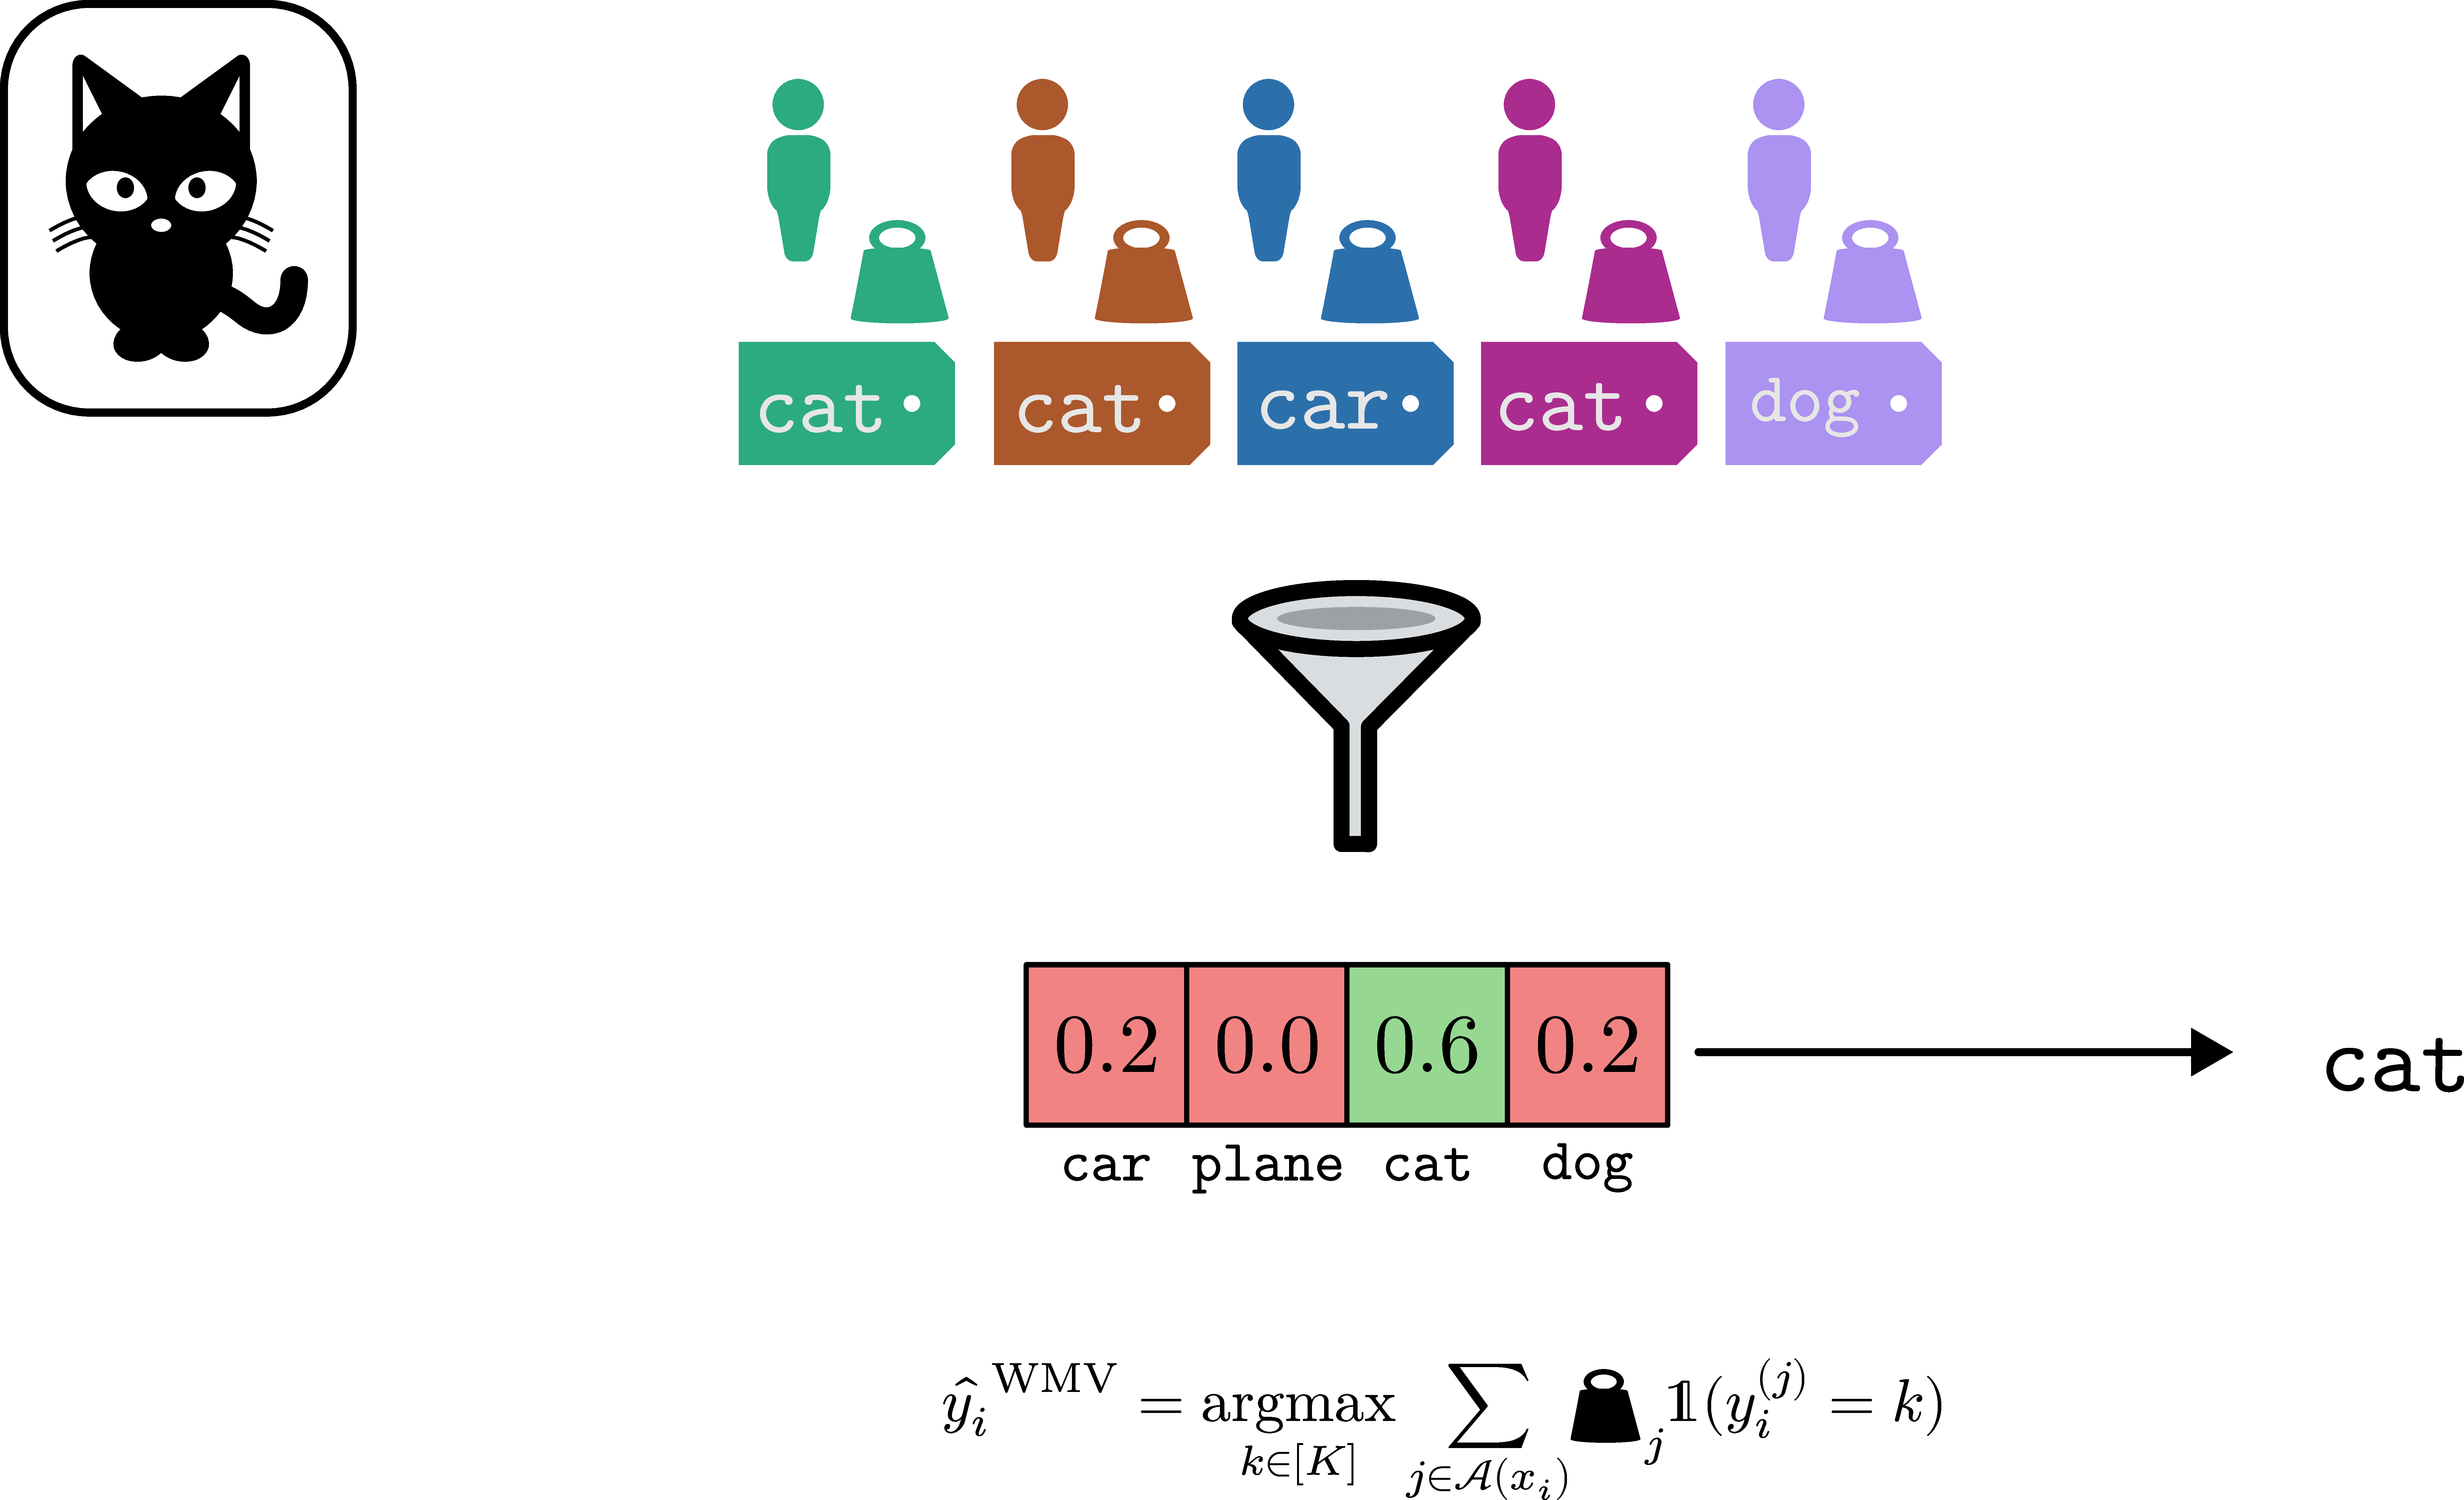
\includegraphics[width=.8\textwidth, clip, trim={50cm 0cm 30cm 80cm}]{./images/MV_label.pdf}
    \end{center}

        For example with balanced weights:

    \begin{center}
        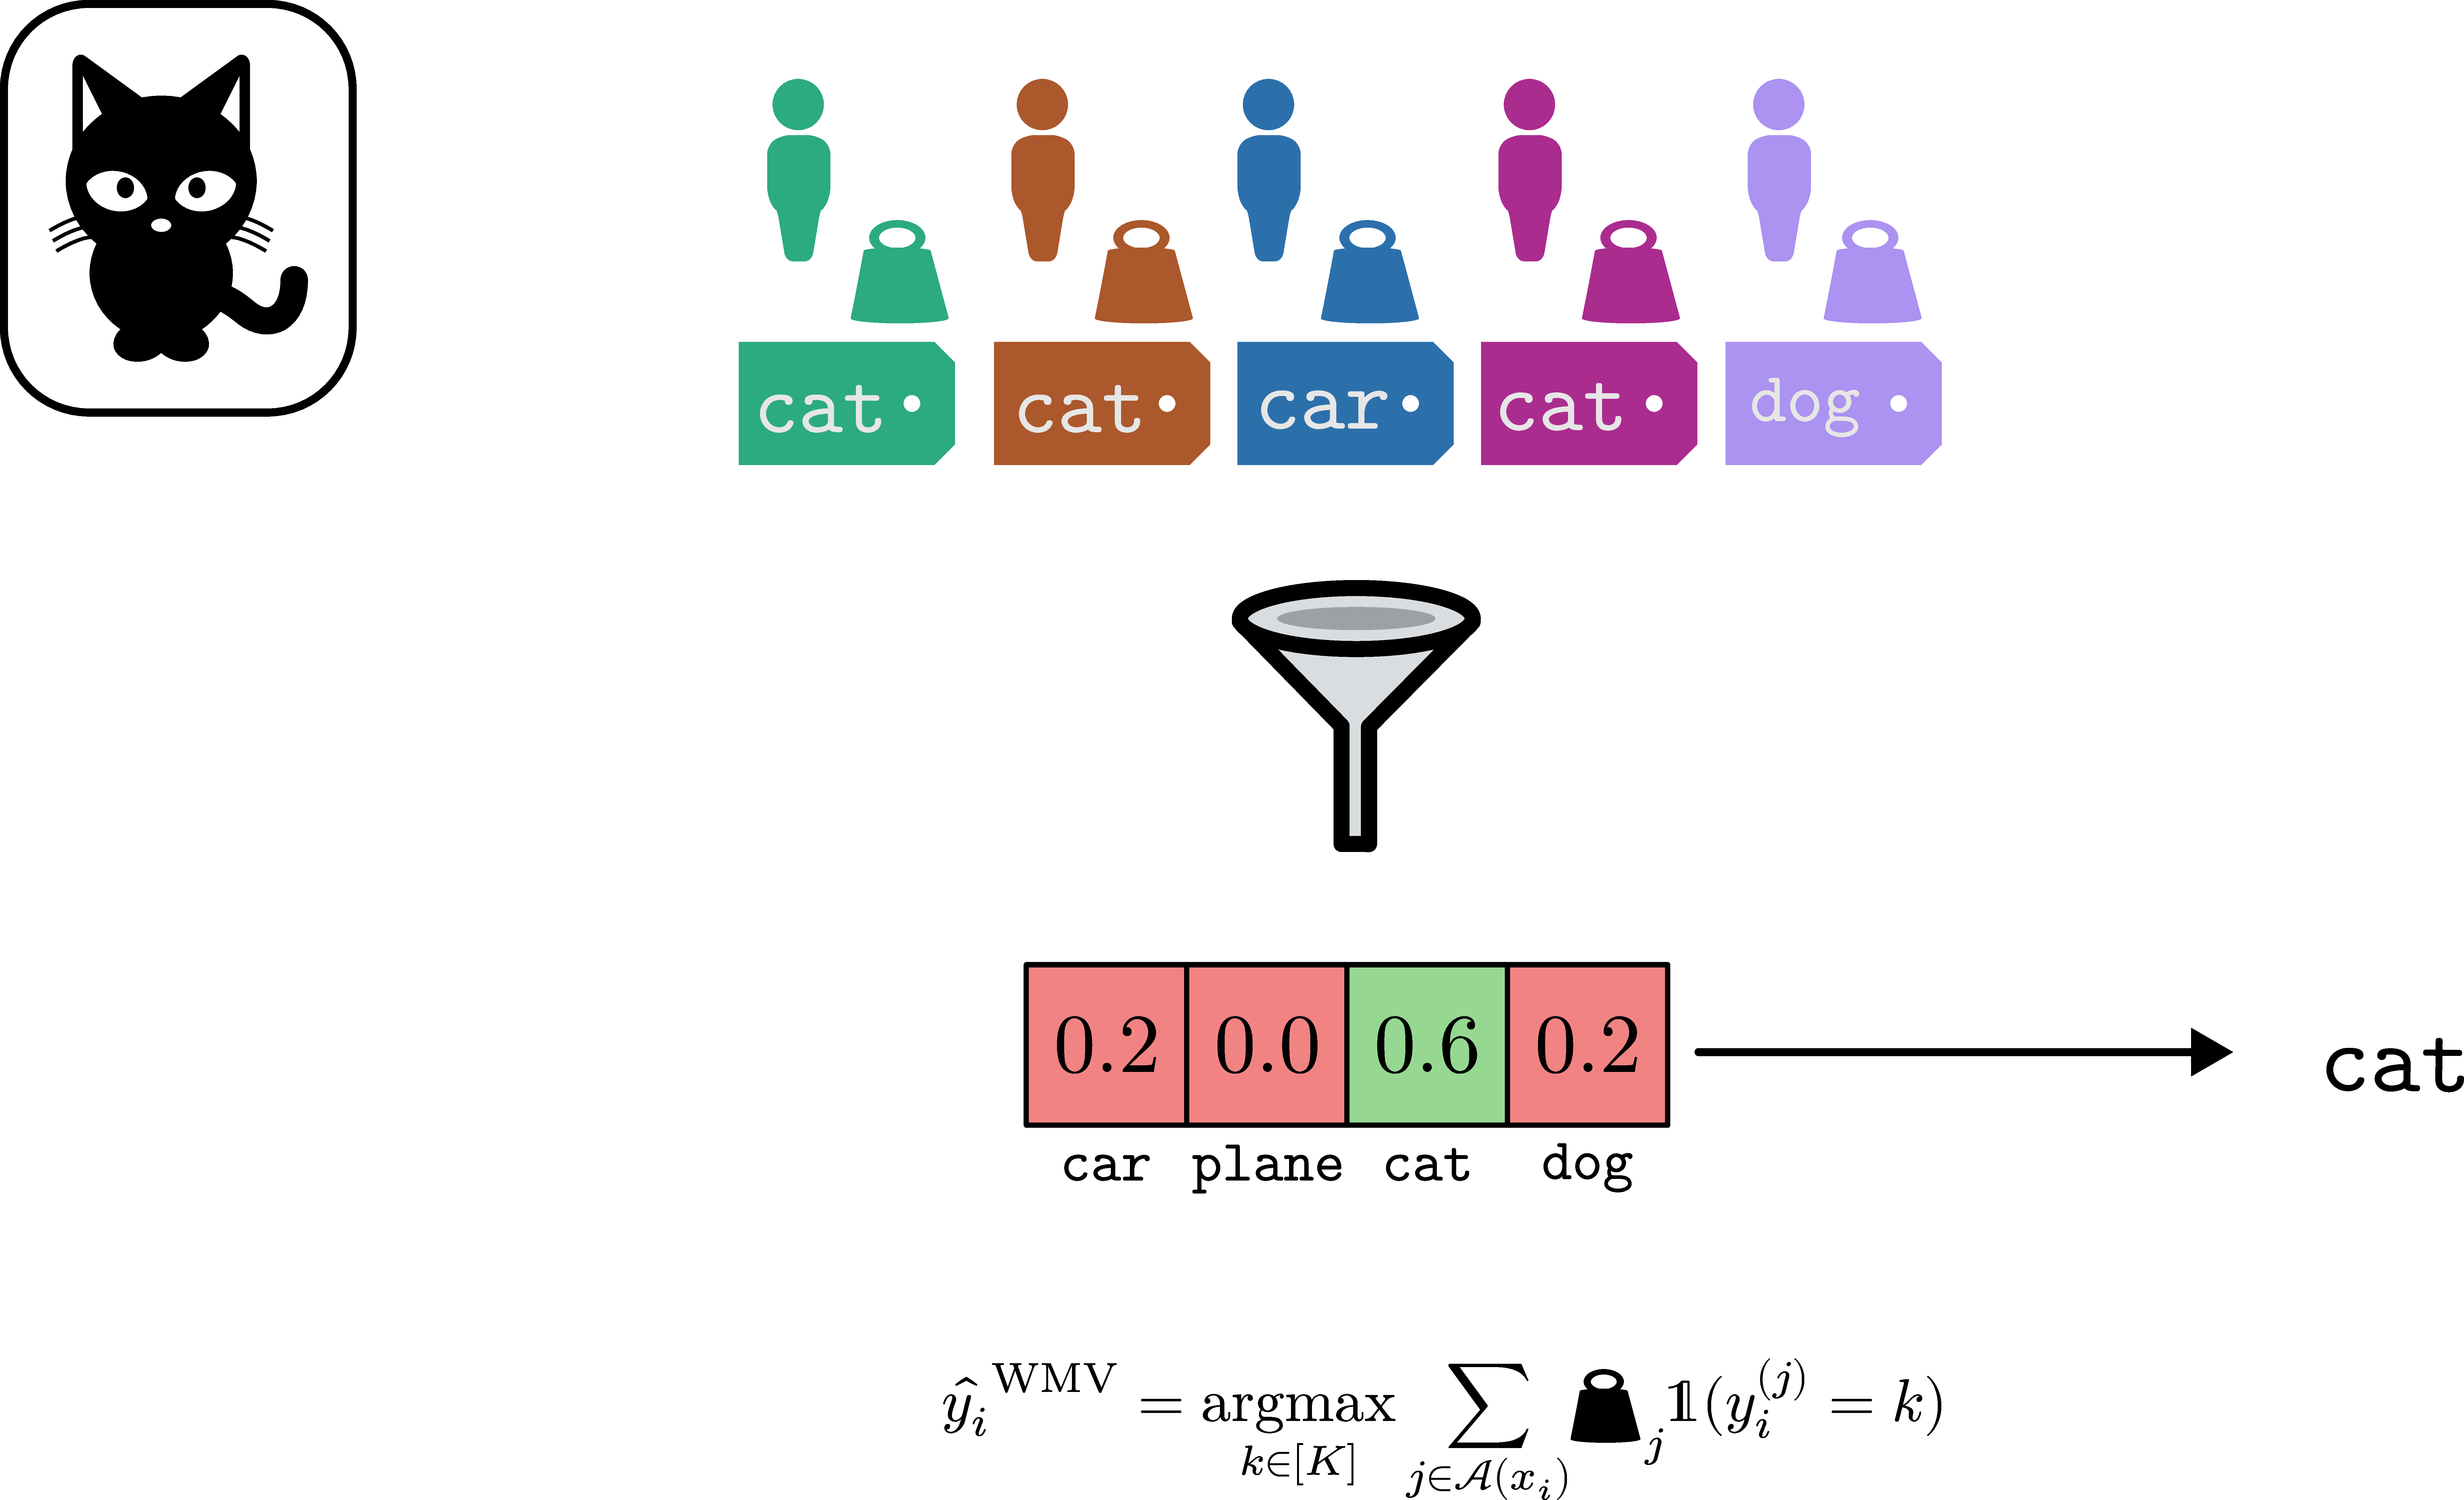
\includegraphics[width=\textwidth, clip, trim={0cm 10cm 0cm 0cm}]{./images/MV_label.pdf}
    \end{center}

\end{frame}
%%%%%%%%%%%%%%%%%%%%%%%%%%%%%%%%%%%%%%%%%%%%%%%%%%%%%%%%%%%%%%%%%%%%%%%%%%%%%%%

\begin{frame}{Classical aggregation strategy}{(Weighted) Majority Votes}
    \begin{center}
        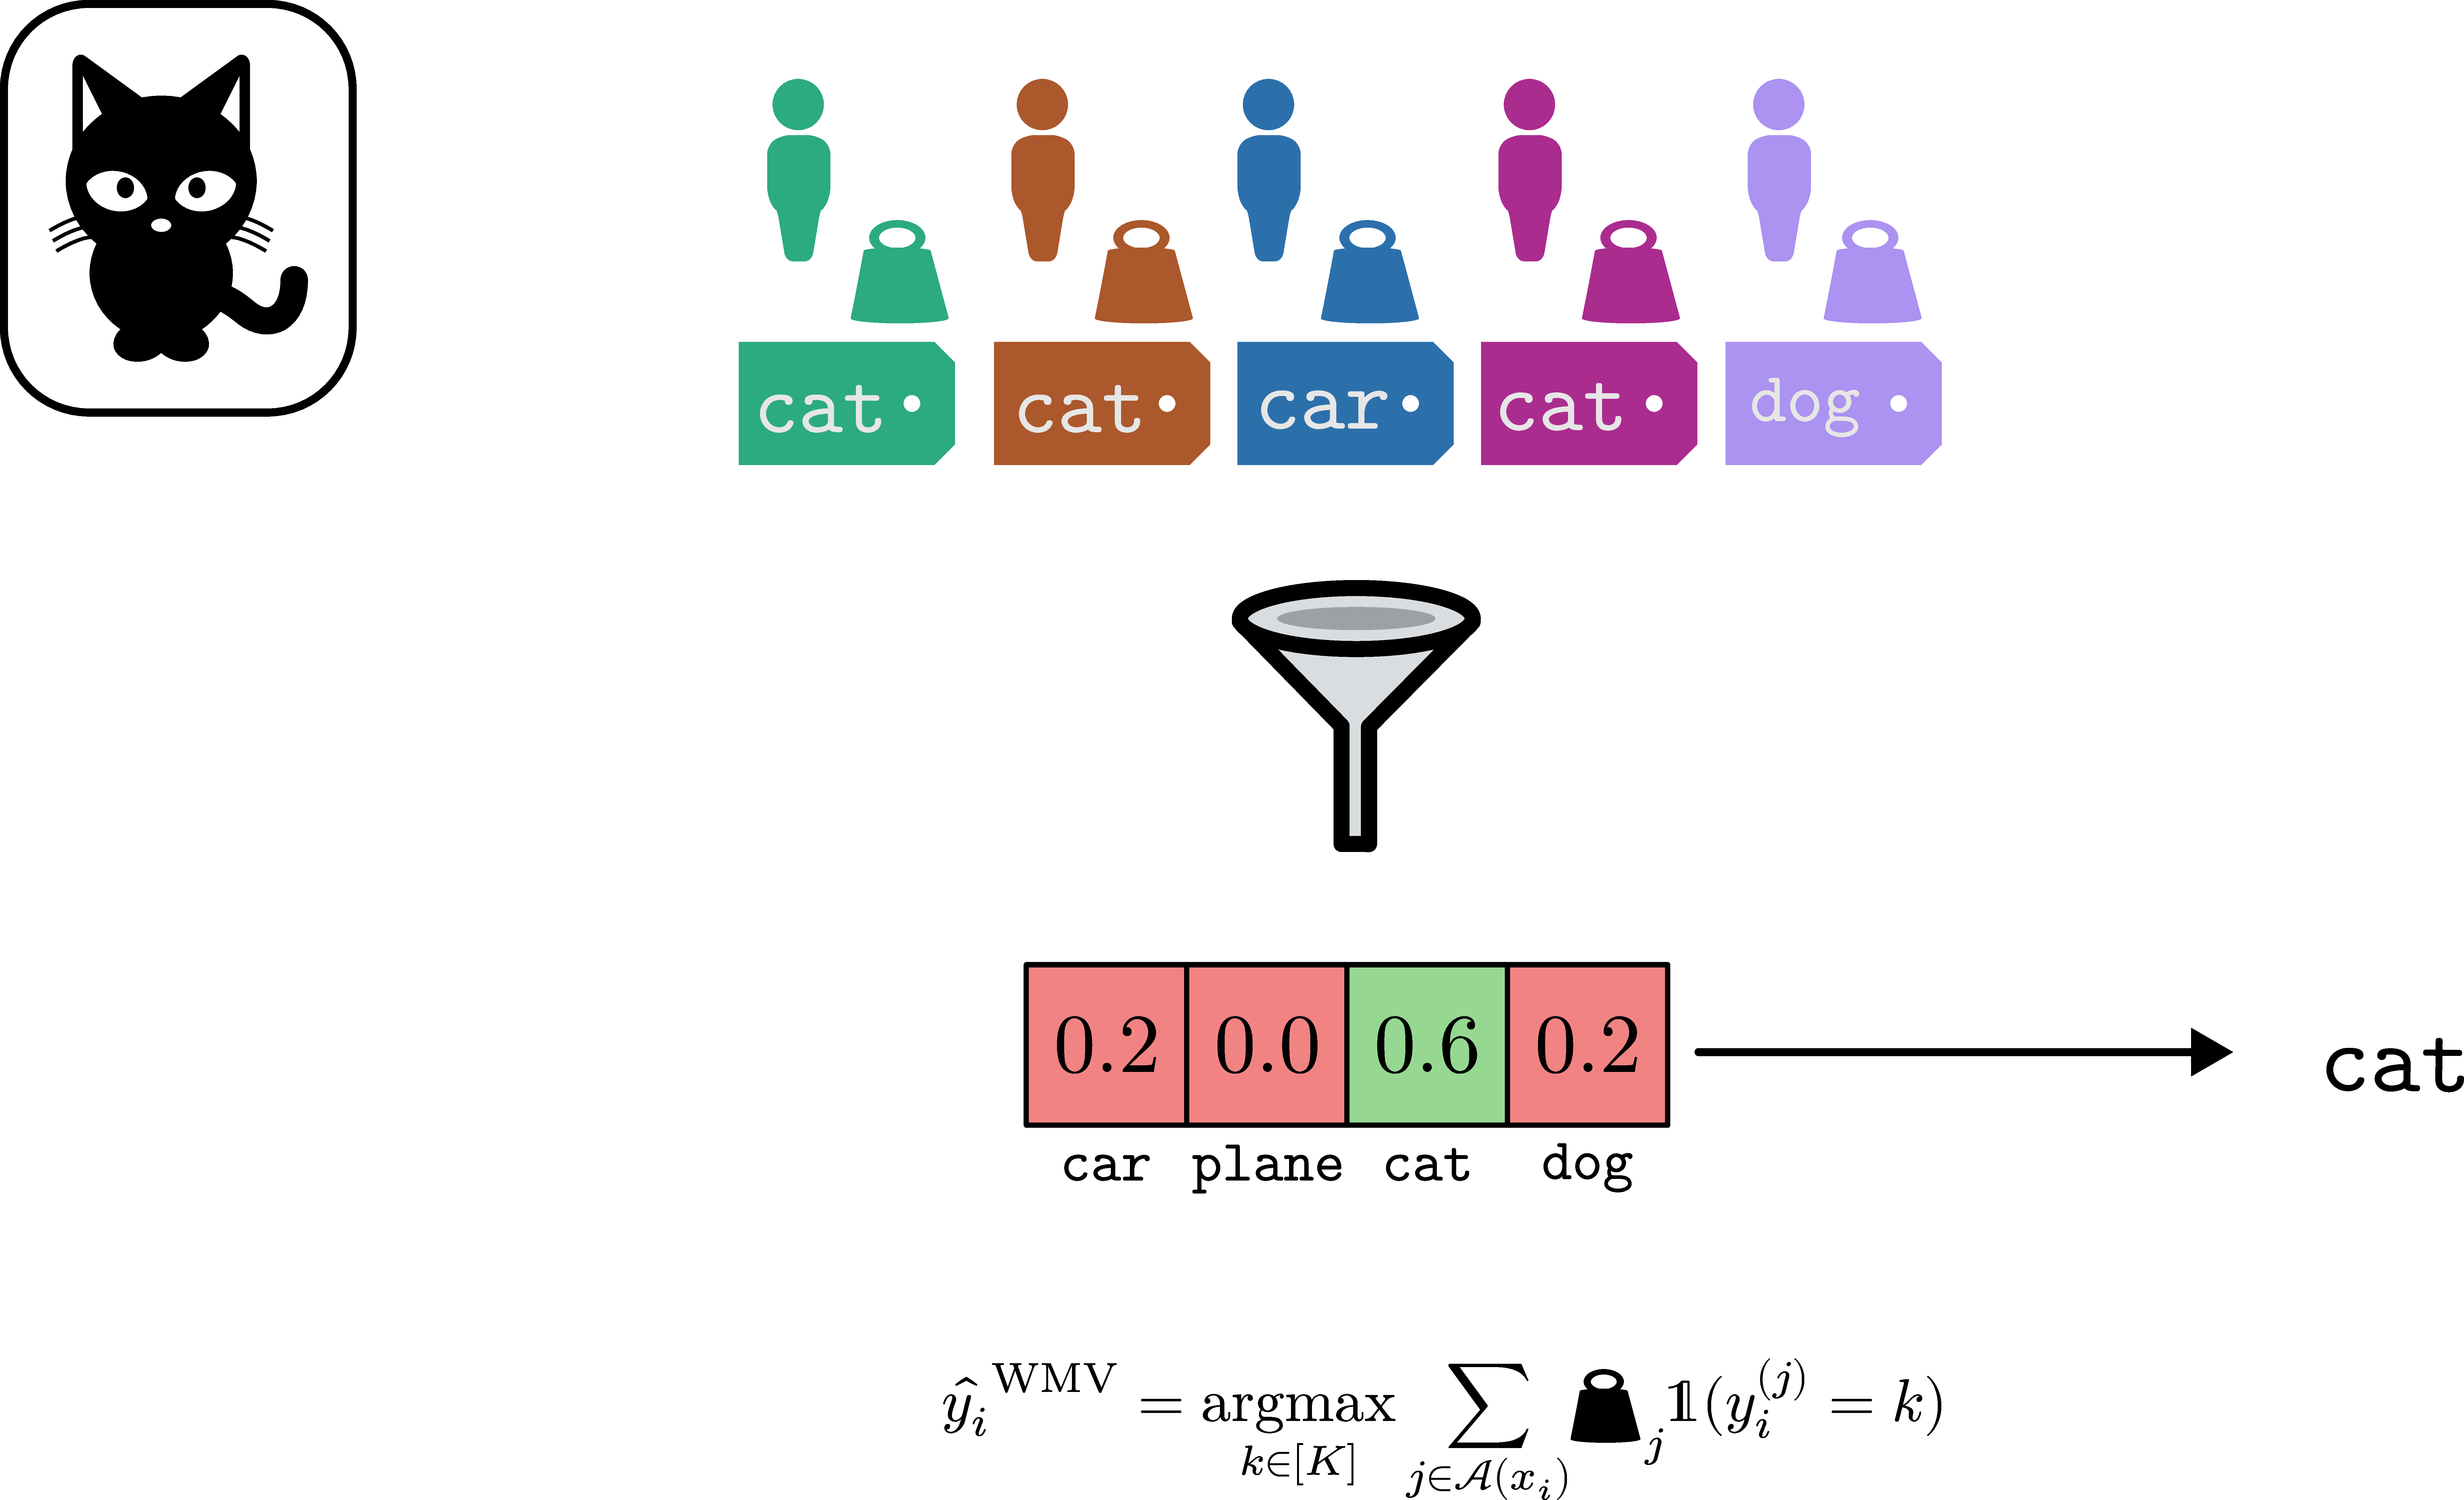
\includegraphics[width=.8\textwidth, clip, trim={50cm 0cm 30cm 80cm}]{./images/MV_label.pdf}
    \end{center}

        For example with unbalanced weights:

    \begin{center}
        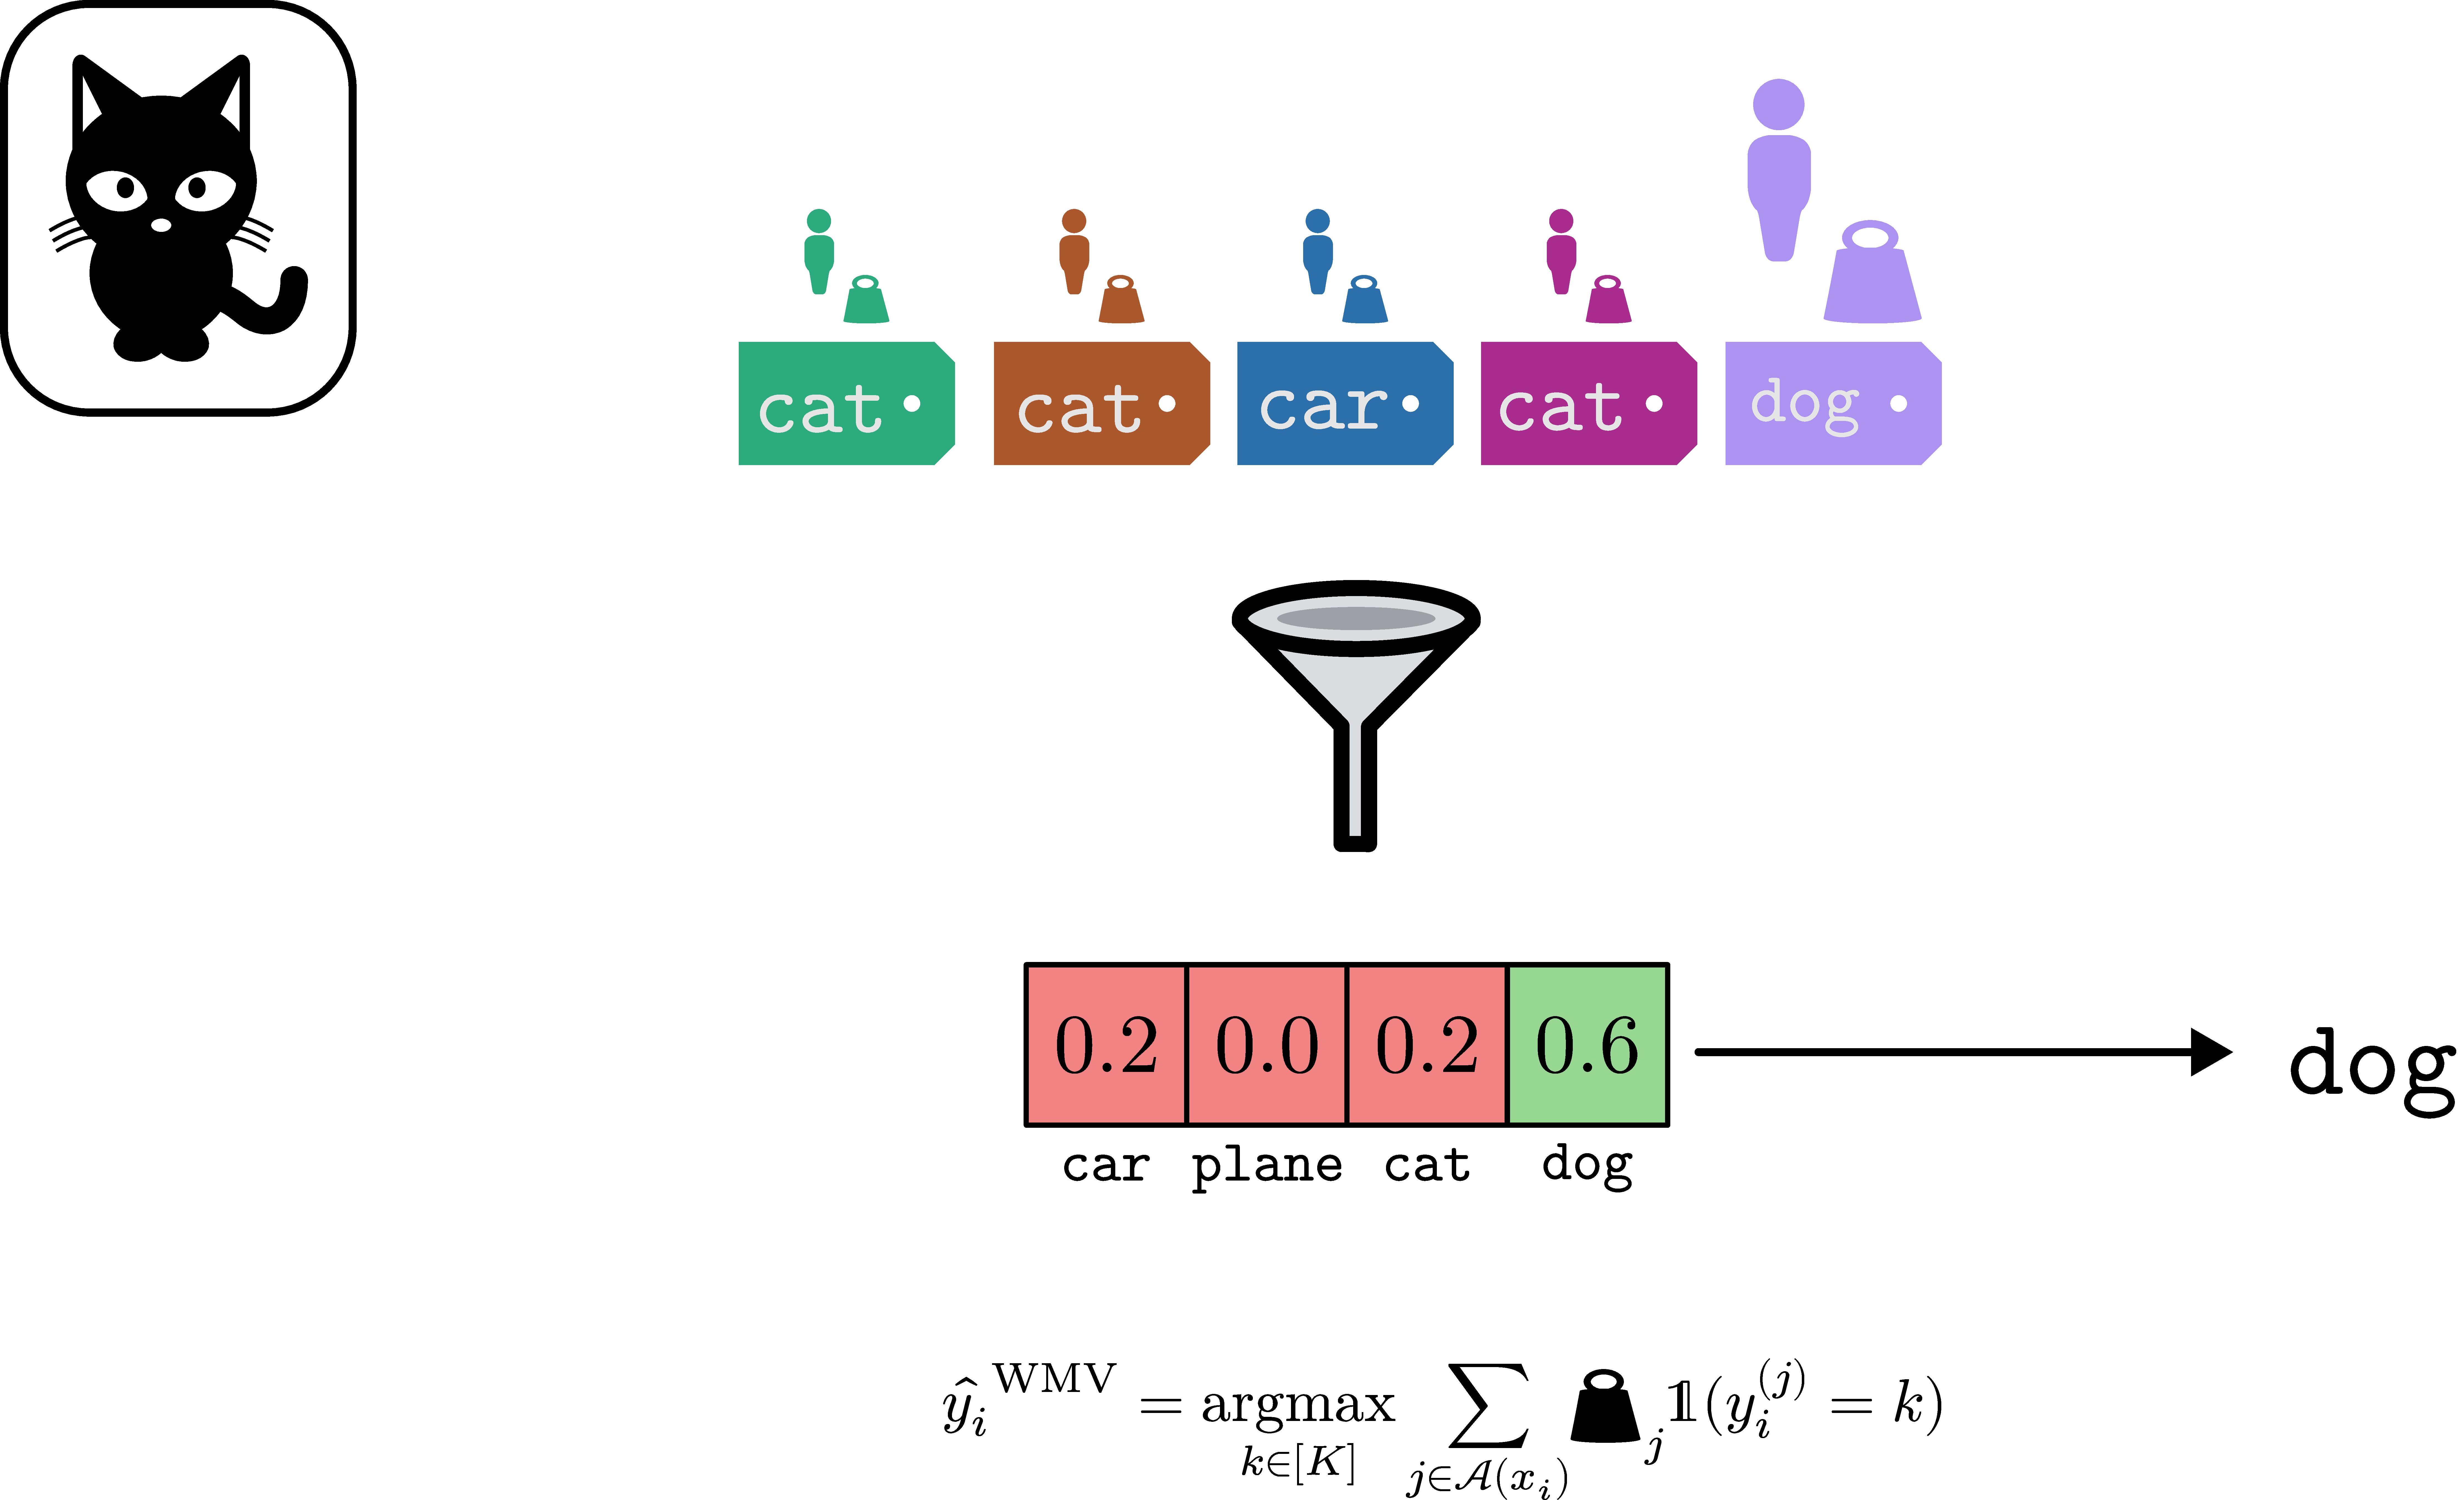
\includegraphics[width=\textwidth, clip, trim={0cm 10cm 0cm 0cm}]{./images/MV_label_unbalanced.pdf}
    \end{center}

\end{frame}


%%%%%%%%%%%%%%%%%%%%%%%%%%%%%%%%%%%%%%%%%%%%%%%%%%%%%%%%%%%%%%%%%%%%%%%%%%%%%%%
\begin{frame}{Classical aggregation strategy}{(Weighted) Majority Votes}
Many existing weight choices:
\begin{itemize}[itemsep=15pt]
    \item Inter worker agreement: WAWA \footnote{\url{https://success.appen.com/hc/en-us/articles/202703205-Calculating-Worker-Agreement-with-Aggregate-Wawa}}:
    \[
    \mathrm{weight}(w_j) = \mathrm{Accuracy}(\{y_i^{(j)}\}_i, \{\hat {y_i}^\mathrm{MV}\}_i)
    \]
    \item Feature importance + game theory: Shapley-value weight\footfullcite{lefort:hal-04573727}
    \item Matrix completion: MACE\footfullcite{hovy2013learning} \dots
\end{itemize}
\vspace{1cm}
\textbf{Pros:} "simple" weight can scale to large datasets and be easy to interpret

\textbf{Cons:} Can not capture worker skills in detail
\end{frame}
%%%%%%%%%%%%%%%%%%%%%%%%%%%%%%%%%%%%%%%%%%%%%%%%%%%%%%%%%%%%%%%%%%%%%%%%%%%%%%%


\begin{frame}{Classical aggregation strategy}{Dawid and Skene\footfullcite{dawid_maximum_1979}}
\begin{itemize}
    \item Introduced in a medical context (aggregate multiple diagnosis)
    \item Represent worker $j$ from their pairwise confusions matrix $\pi^{(j)}\in\mathbb{R}^{K\times K}$
    \item Probabilistic model on their answers:
    \[
    y^{(j)} | y^\star \sim \mathrm{Multinomial}(\pi^{(j)}_{y^\star, \bullet})
    \]
    with $\pi^{(j)}_{k,\ell}=\mathbb{P}(\text{worker }j \text{ answers }\ell \text{ with unknown truth } k)$
\end{itemize}
\vspace{.5cm}
\begin{columns}
    \begin{column}{.45\textwidth}
    \textbf{Pros:}
    \begin{itemize}
        \item Finer modelisation
        \item Can use adversarial workers
    \end{itemize}
    \end{column}
    \begin{column}{.45\textwidth}
        \textbf{Cons:}
        \begin{itemize}
            \item Memory issue: $n_{\texttt{worker}}\times K^2$ parameters to estimate only the confusion matrices
        \end{itemize}
    \end{column}
\end{columns}
\end{frame}

\begin{frame}{Classical aggregation strategy}{Dawid and Skene -- Model}
Probabilistic model $\longrightarrow$ Likelihood (to maximize via the Expectation Maximization algorithm)
% \[
%     \displaystyle\prod_{i\in [n_{\texttt{task}}]}\prod_{k \in [K]}\bigg[\rho_k\prod_{j\in [n_{\texttt{worker}}]}
%     \prod_{\ell\in [K]}\big(\pi^{(j)}_{k, \ell}\big)^{\mathds{1}_{\{y_i^{(j)}=\ell\}}}
%     \bigg]^{T_{i,k}},
% \]
% $\rho_k=\mathbb{P}(y_i^\star=k)$ the prevalence and $T_{i,k}=\mathds{1}(y_i^\star=k)$ the estimated labels
% \vspace{.5cm}
\begin{center}
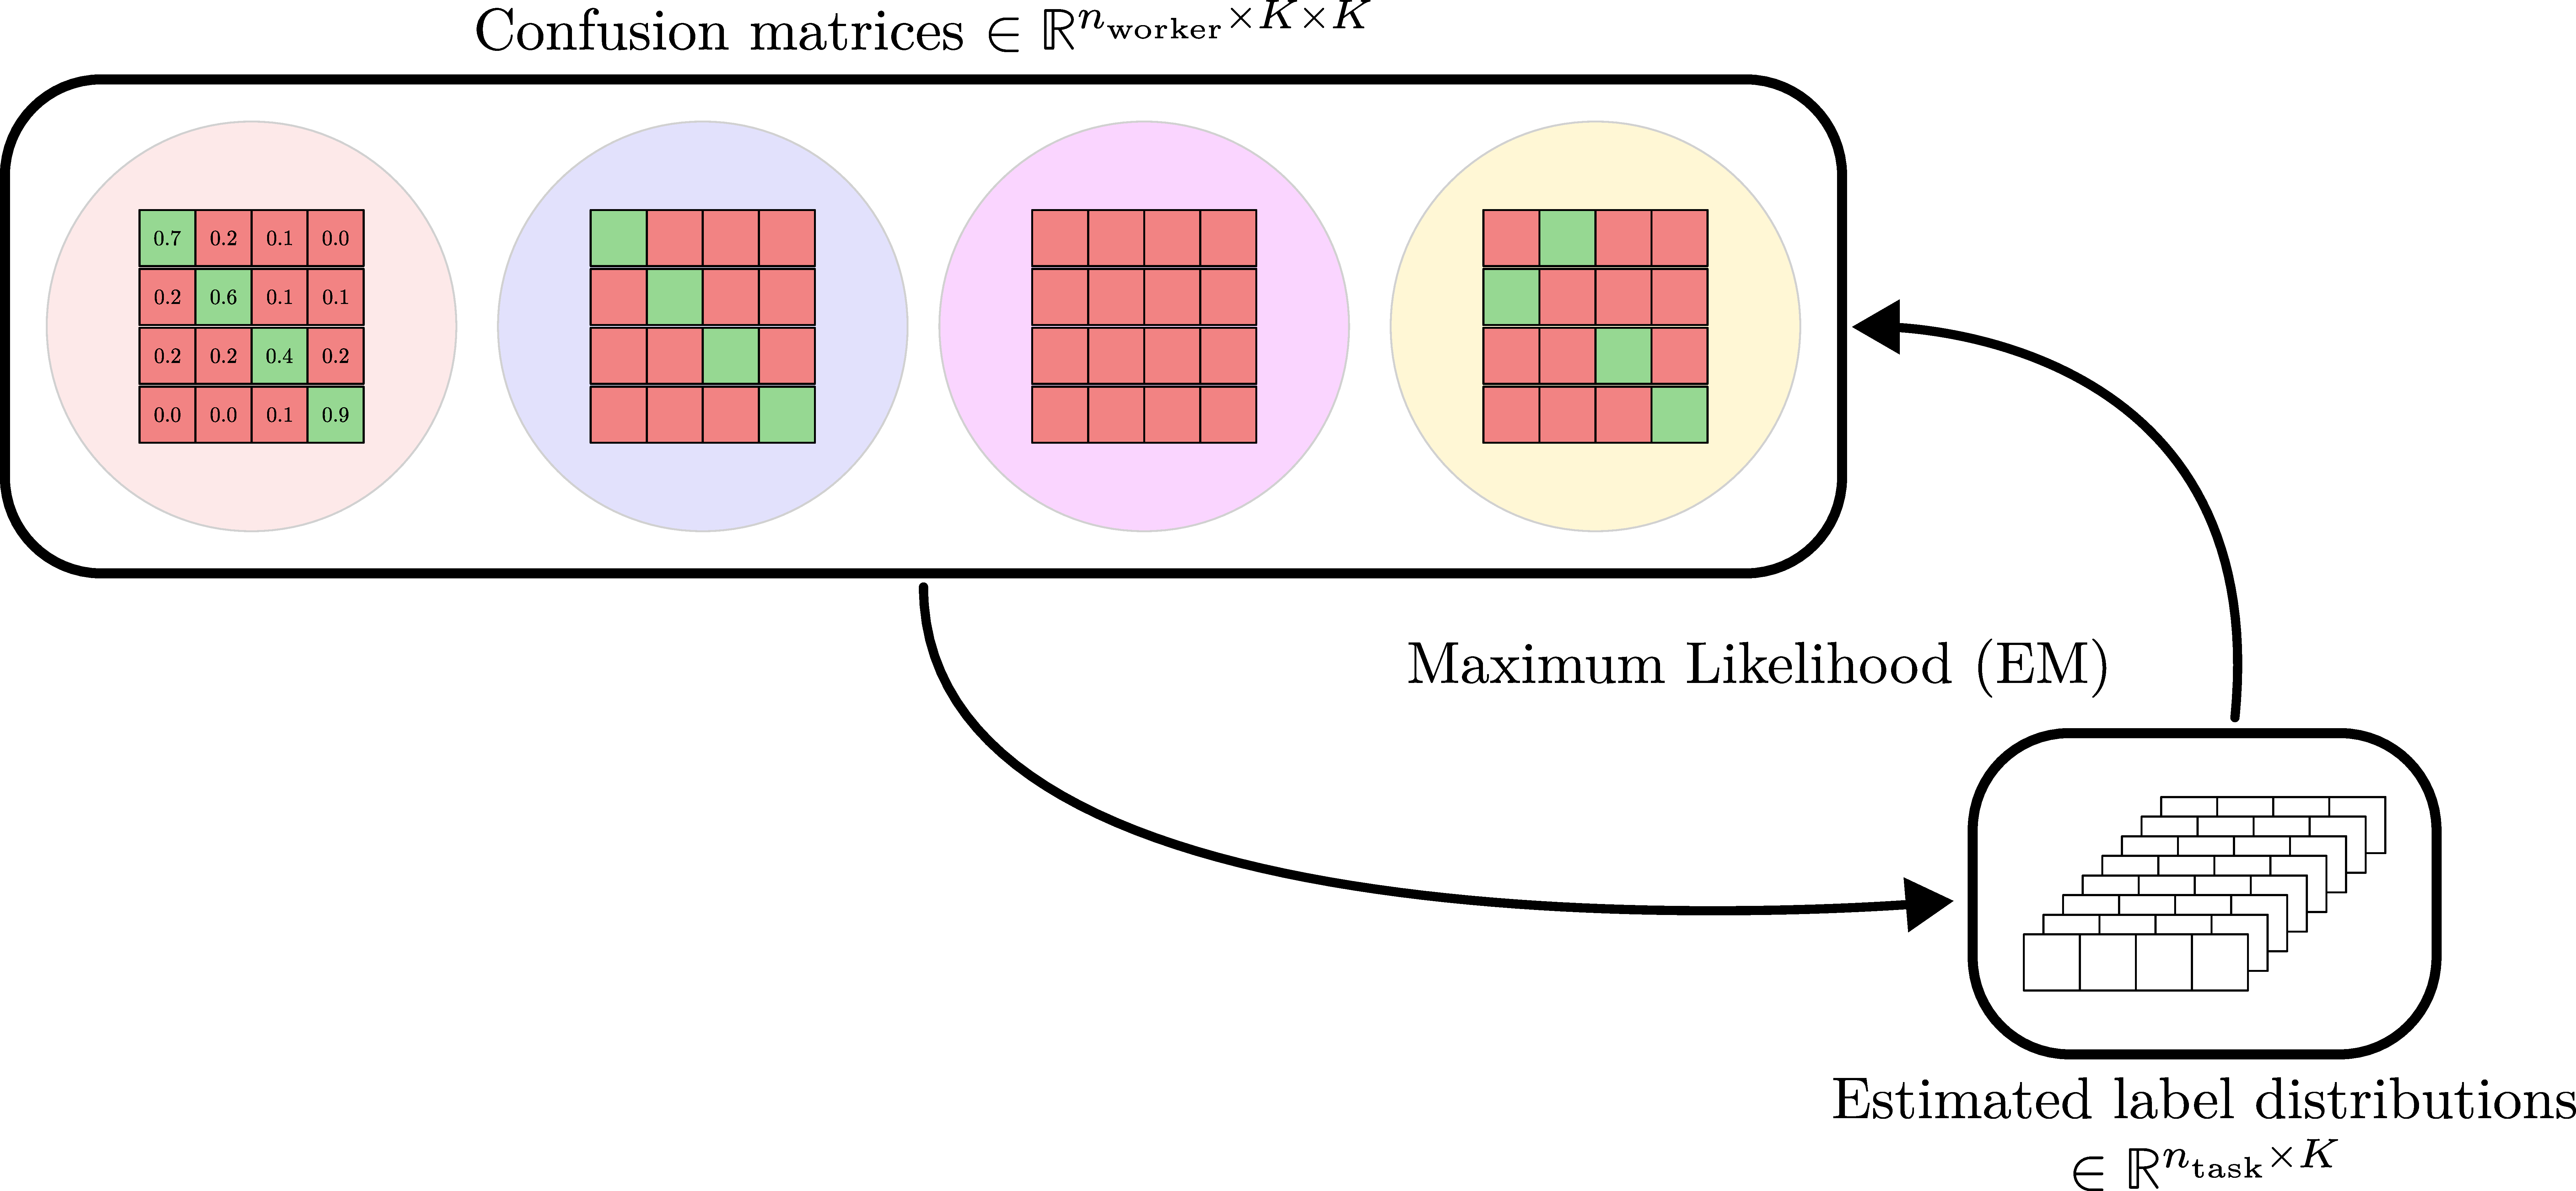
\includegraphics[width=.75\textwidth]{./images/DS_EM.pdf}
\end{center}
\end{frame}

\begin{frame}{Classical deep-learning strategy}{CrowdLayer\footfullcite{rodrigues2018deep}}
    \begin{itemize}
        \item Idea: put the DS confusion matrix in a neural network as a new layer
    \end{itemize}

    \begin{center}
        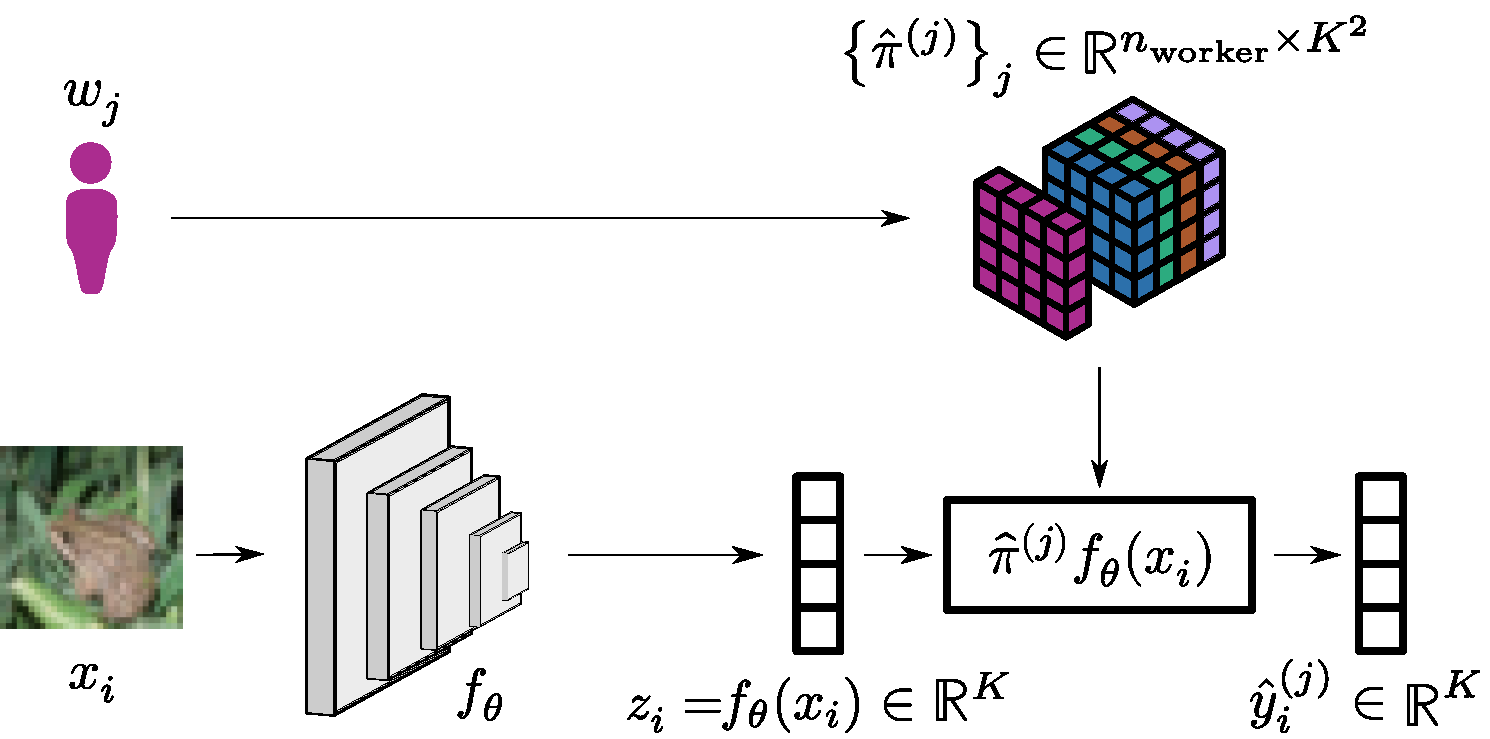
\includegraphics[width=\textwidth]{./images/crowdlayer_scheme.pdf}
    \end{center}
\end{frame}

\begin{frame}{Classical deep-learning strategy}{CoNAL\footfullcite{chu2021learning}}
    \begin{itemize}
        \item Idea: CrowdLayer + global and local confusions
    \end{itemize}
    \begin{center}
        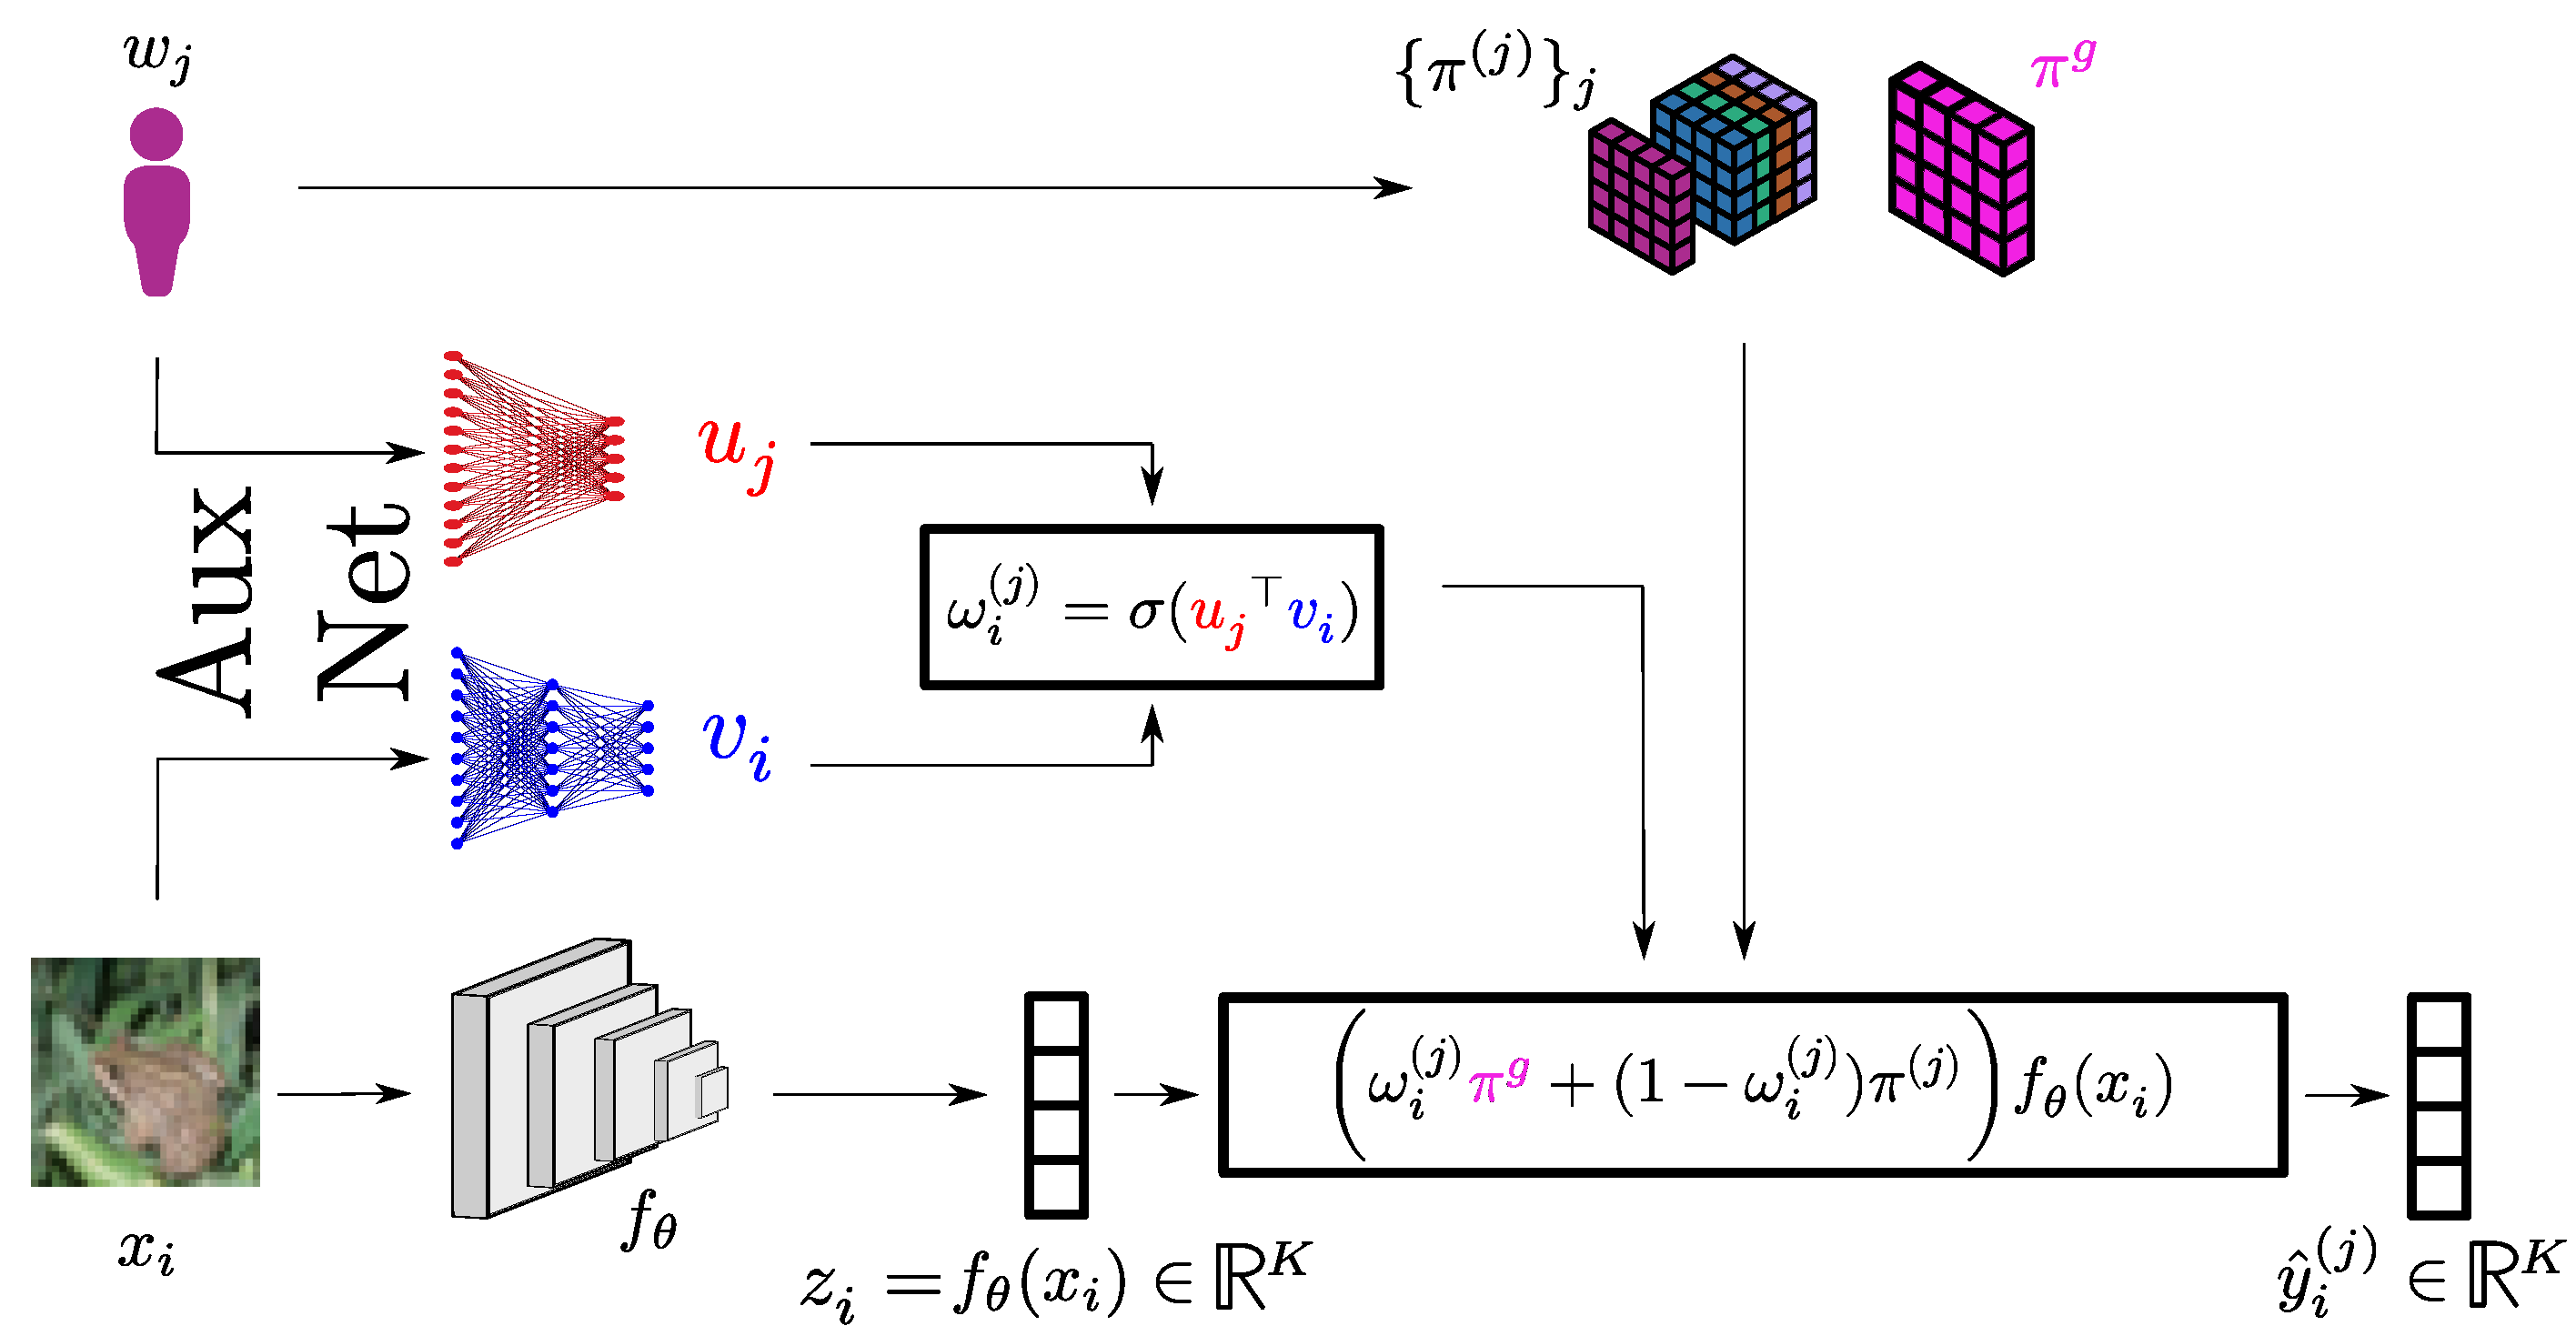
\includegraphics[width=\textwidth]{./images/conal_scheme.pdf}
    \end{center}

\end{frame}

\section{Identify ambiguous tasks in crowdsourced datasets}

%%%%%%%%%%%%%%%%%%%%%%%%%%%%%%%%%%%%%%%%%%%%%%%%%%%%%%%%%%%%%%%%%%%%%%%%%%%%%%%
\begin{frame}{When images have underlying ambiguity}{}
    \begin{onlyenv}<1>
        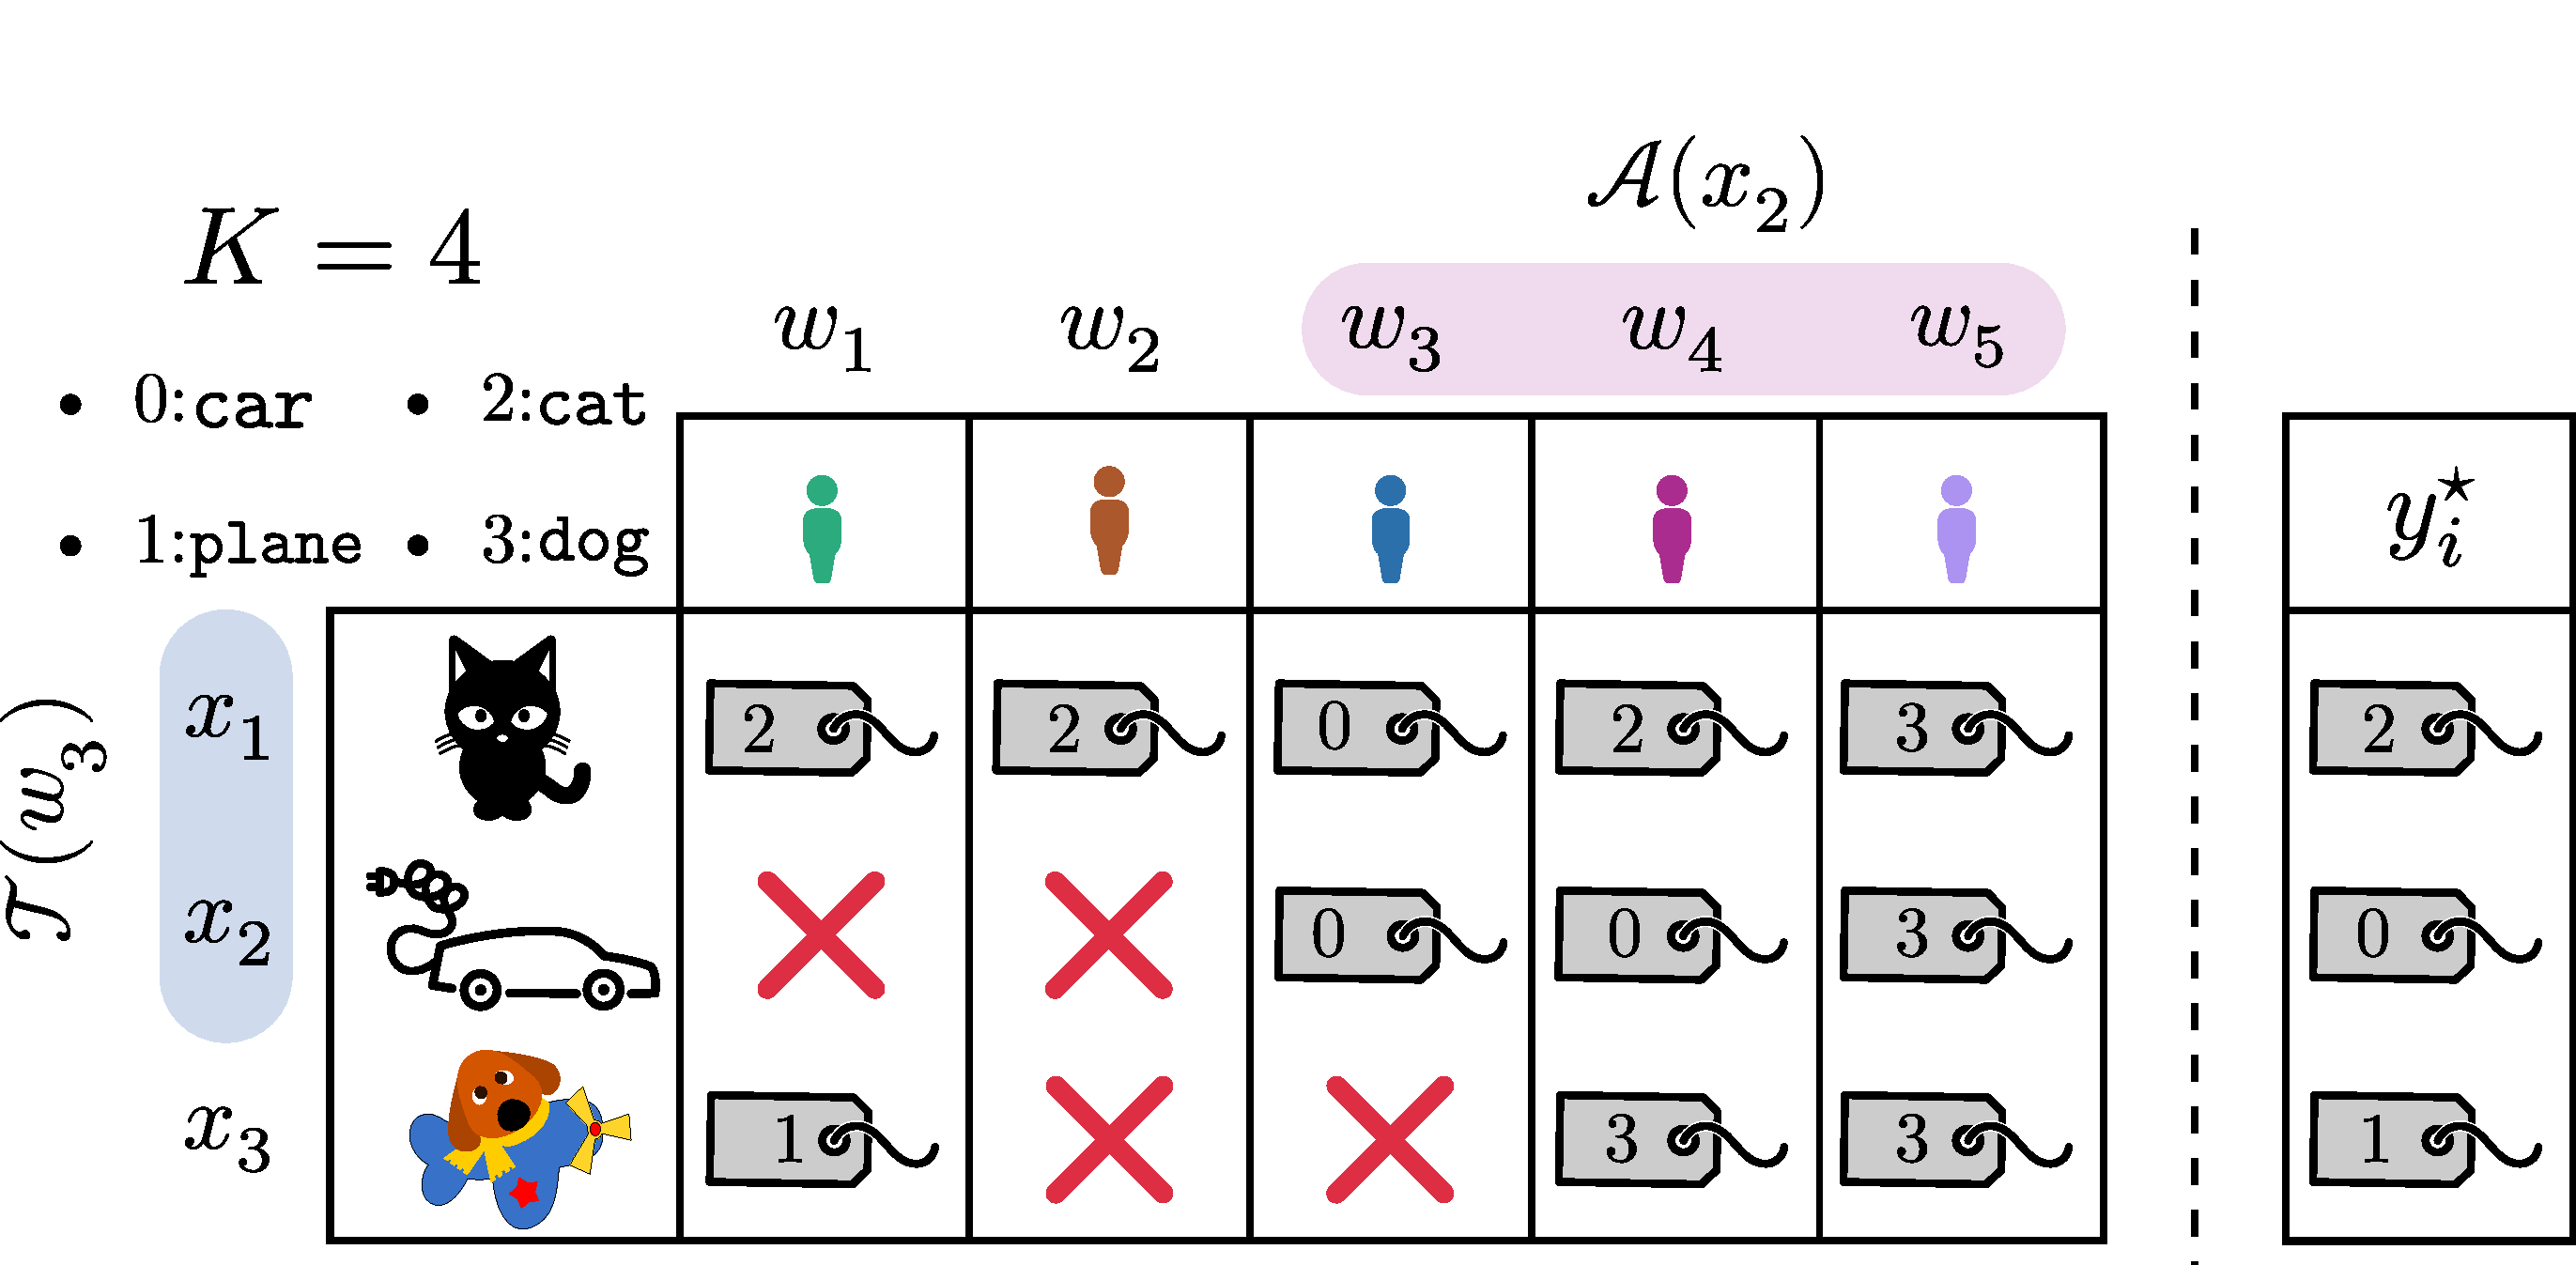
\includegraphics[width=\textwidth, clip,trim={0cm 4cm 0cm 0cm}]{./images/notations_1.pdf}
     \end{onlyenv}
     \begin{onlyenv}<2>
        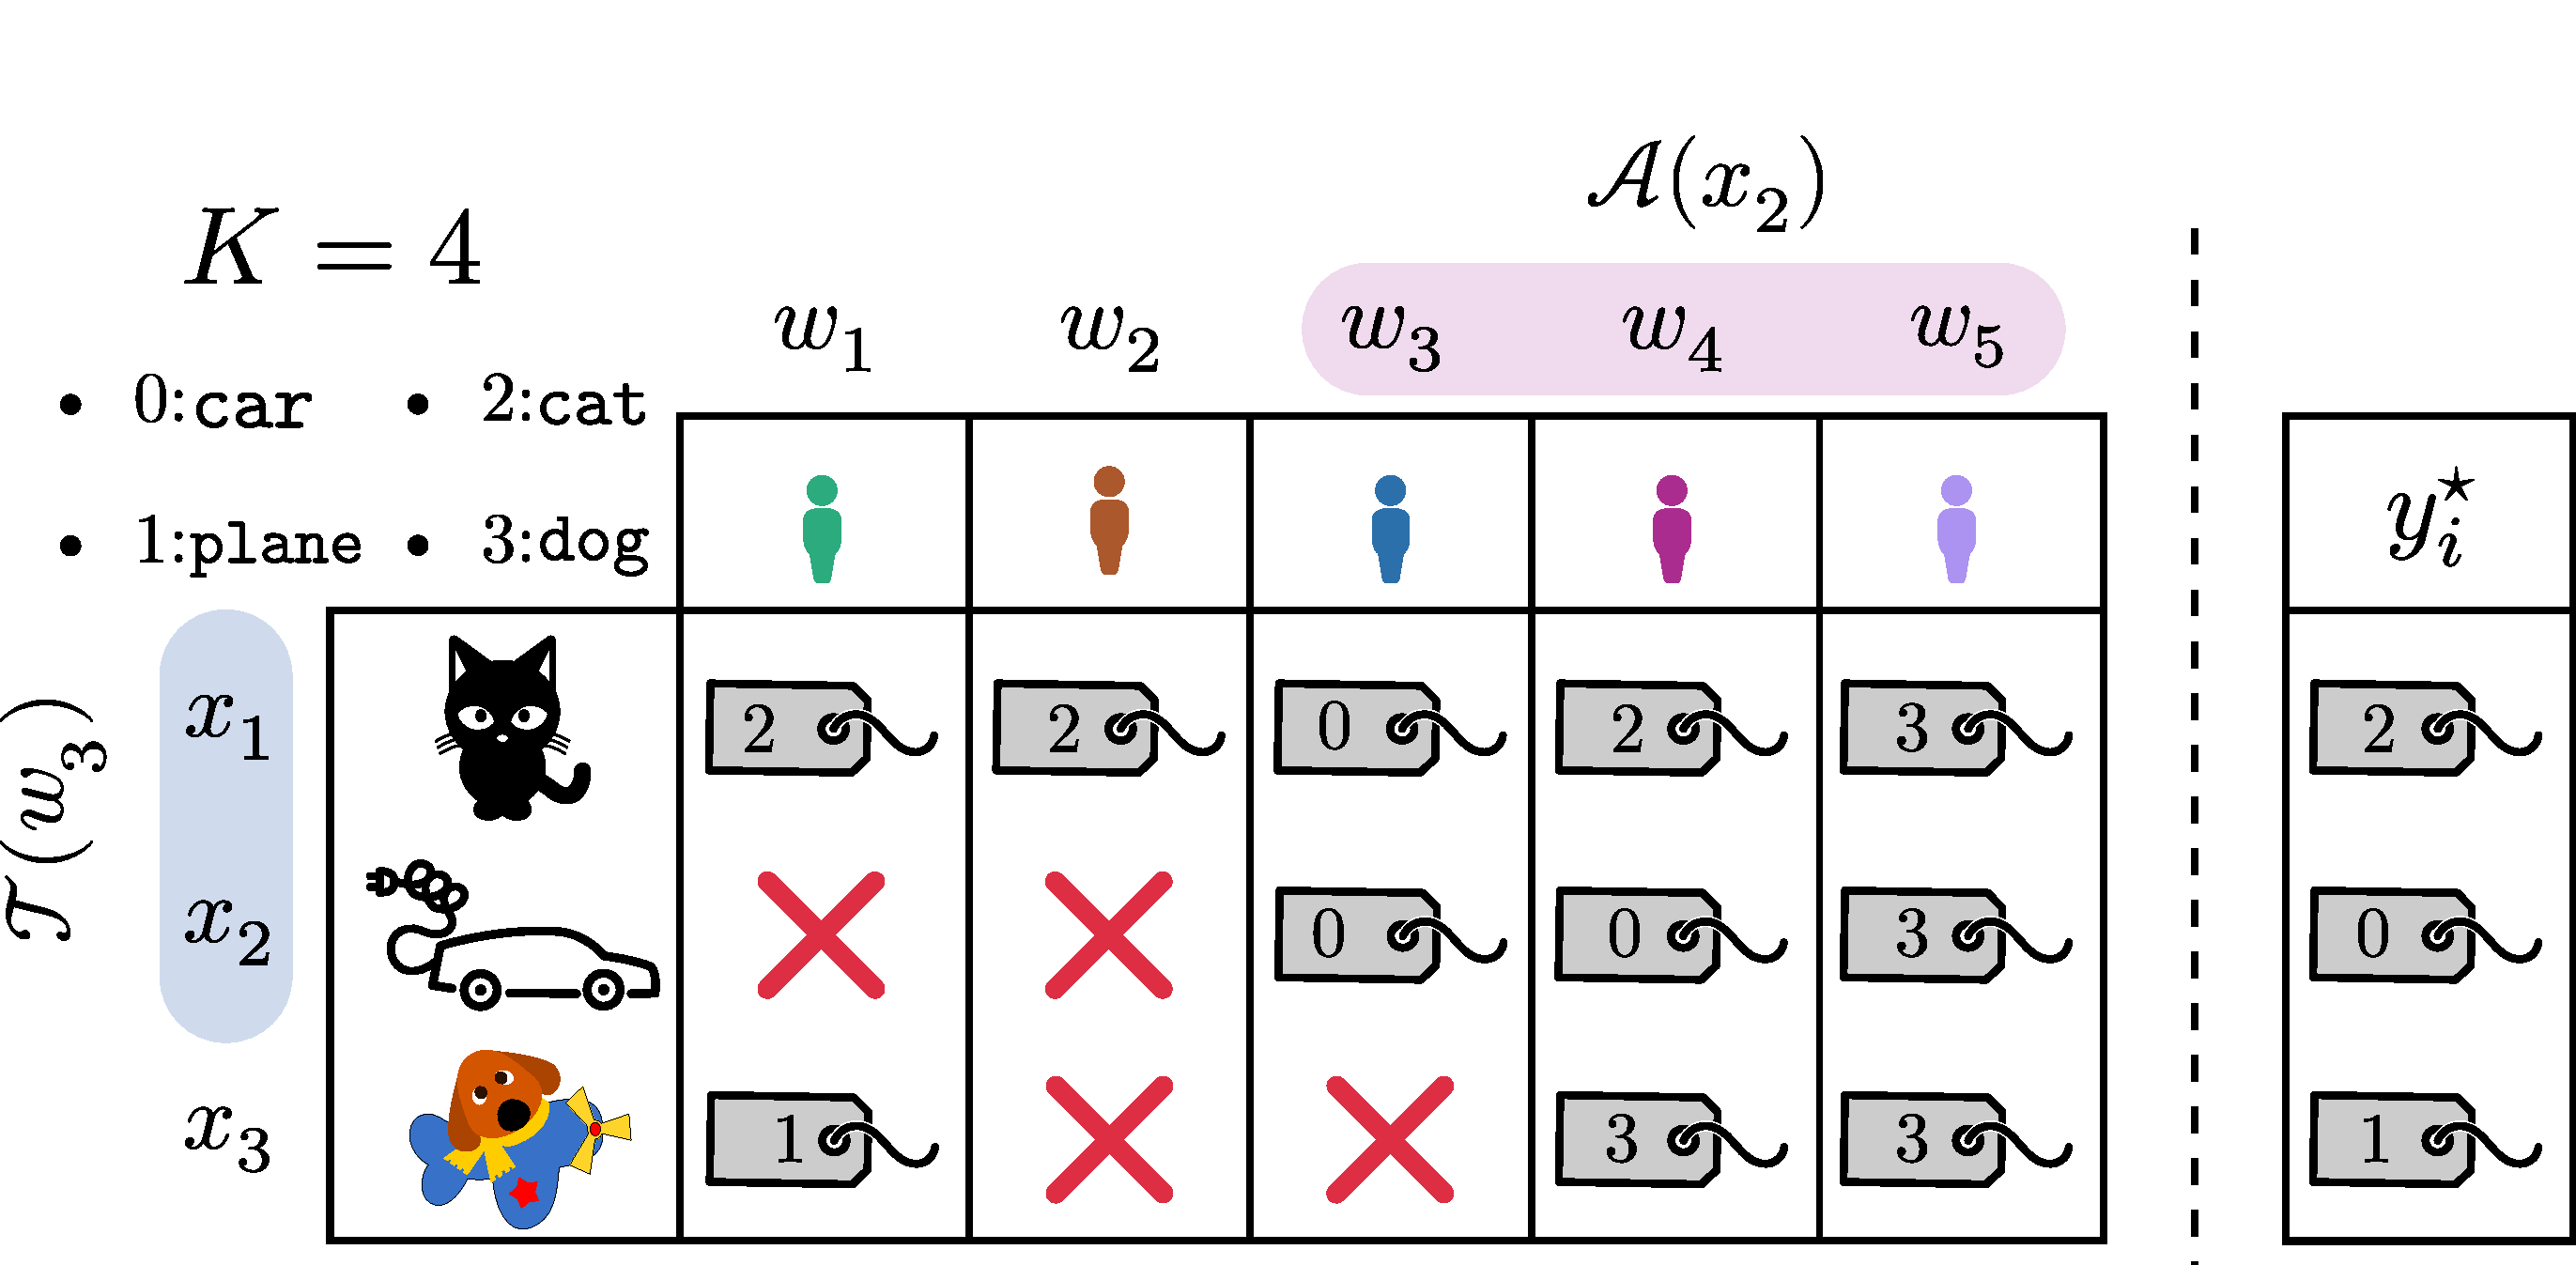
\includegraphics[width=\textwidth]{./images/notations_1.pdf}
    \end{onlyenv}
\end{frame}
%%%%%%%%%%%%%%%%%%%%%%%%%%%%%%%%%%%%%%%%%%%%%%%%%%%%%%%%%%%%%%%%%%%%%%%%%%%%%%%

\begin{frame}{Ambiguity in classical supervised setting}{Area Under the Margin (AUM)}
    \textbf{Goal:} identify issues in classical datasets $(x_1, y_1),\dots,(x_n, y_n)\in \mathcal{X}\times [K]$
\begin{itemize}
    \item AUM\footfullcite{pleiss_identifying_2020}: monitor margin during training
\end{itemize}
\vspace{.5cm}
\begin{columns}
    \begin{column}{.45\textwidth}
        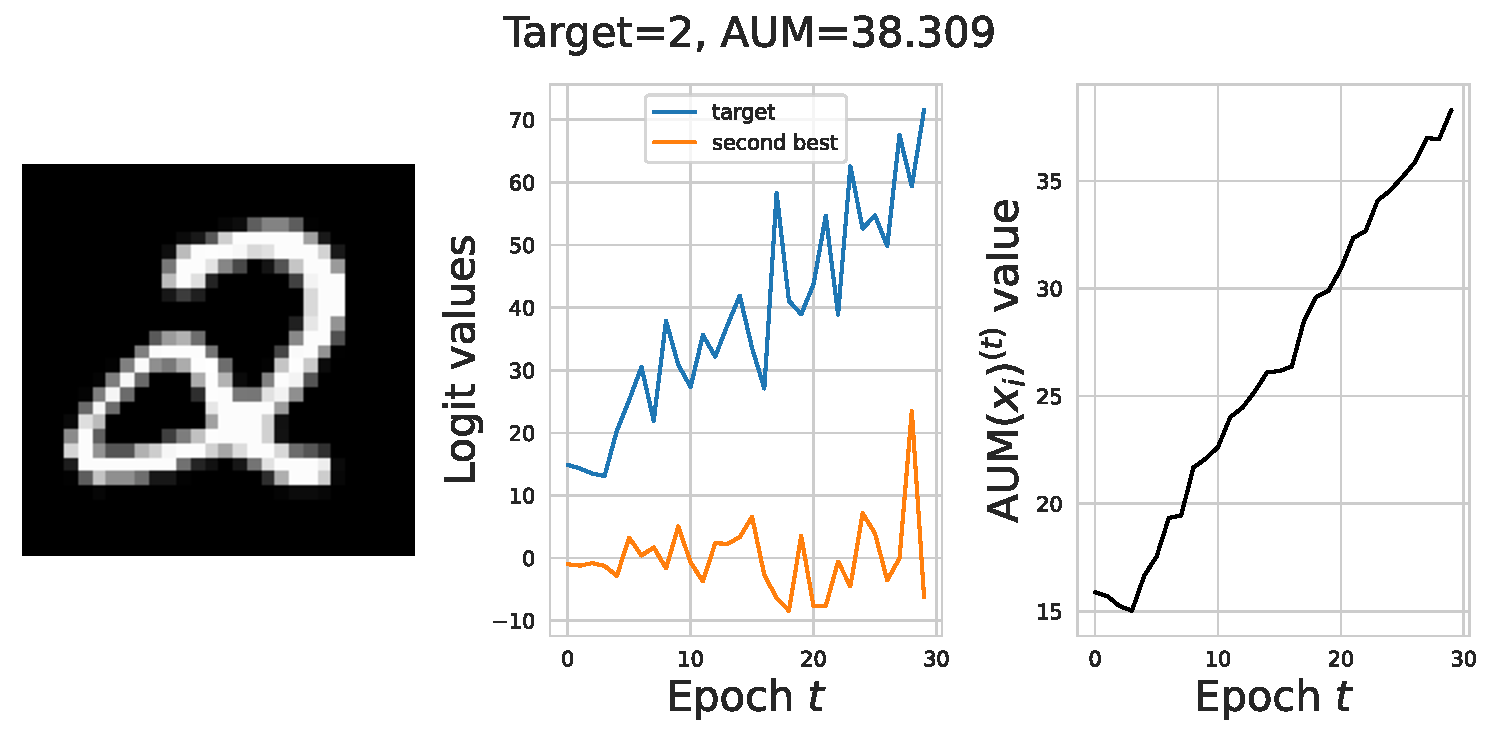
\includegraphics[width=\textwidth]{./../chapters/images/high_aum_mnist.pdf}
    \end{column}
    \begin{column}{.45\textwidth}
        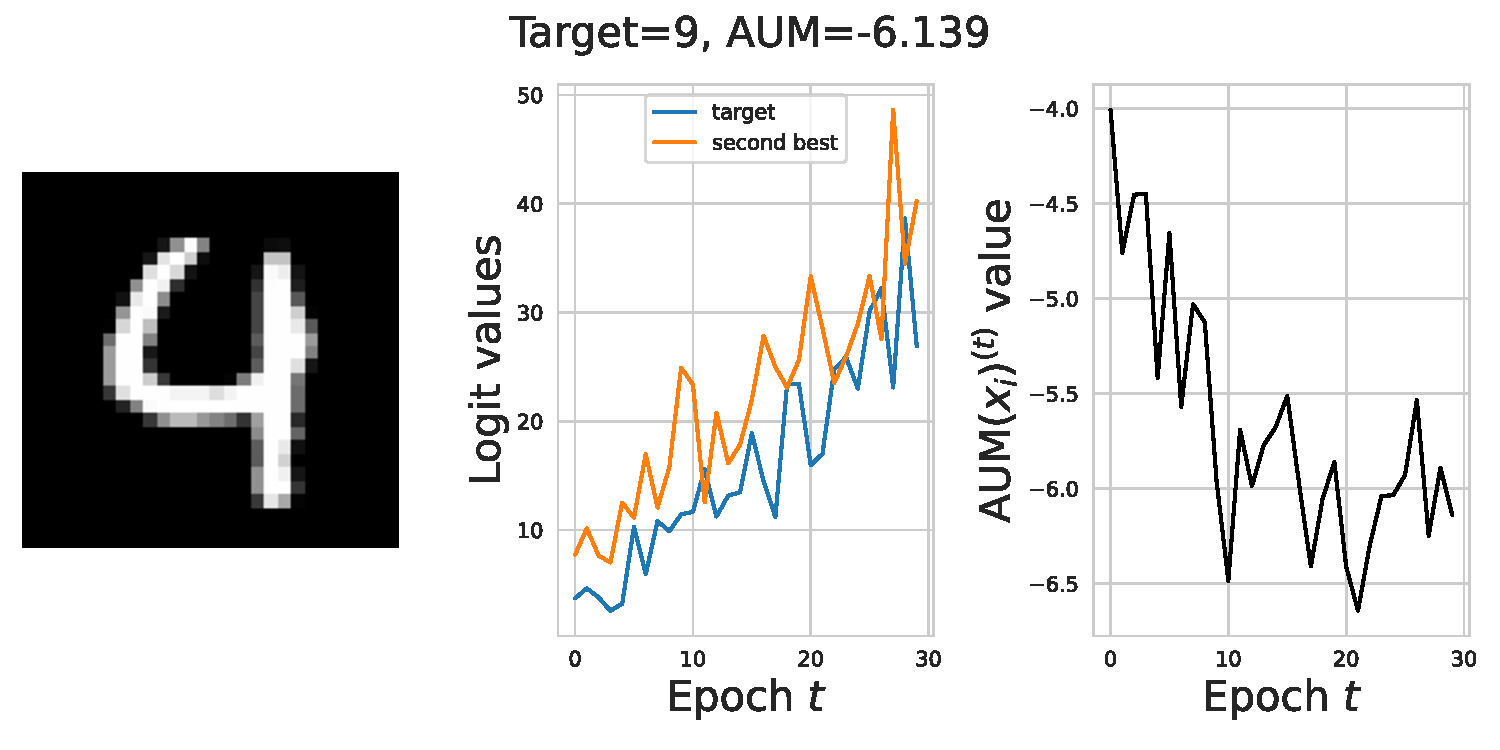
\includegraphics[width=\textwidth]{./../chapters/images/mid_aum_mnist.pdf}
    \end{column}
\end{columns}
\end{frame}
%%%%%%%%%%%%%%%%%%%%%%%%%%%%%%%%%%%%%%%%%%%%%%%%%%%%%%%%%%%%%%%%%%%%%%%%%%%%%%%
\begin{frame}{Ambiguity in classical supervised setting}{Area Under the Margin (AUM)}
    \textbf{Goal:} identify issues in classical datasets $(x_1, y_1),\dots,(x_n, y_n)\in \mathcal{X}\times [K]$
\begin{itemize}
    \item AUM\footfullcite{pleiss_identifying_2020}: monitor margin during training
    \item Classifier: at training epoch $t \in [T]$, $\mathcal{C}^{(t)}(x_i)\in\mathbb{R}^K$ a vector of \textcolor{red}{scores} (logits)
\end{itemize}

\vspace{0.2cm}

\begin{equation*}
    \mathrm{AUM}(x_i, y_i) =
    \tikzmarknode{avg}{\highlight{purple}{
            \color{black}
            $\displaystyle\frac{1}{T} \sum_{t=1}^T$
        }}
    \color{purple}
    \overbrace{
        \Bigg[
            \tikzmarknode{scorelabel}{\highlight{blue}{ \color{black}
                    $\mathcal{C}^{(t)}(x_i)_{y_i}$
                }}
            -
            \tikzmarknode{scoremax}{\highlight{gray}{ \color{black}
                    $\displaystyle\max_{\ell \neq y_i}\mathcal{C}^{(t)}(x_i)_\ell$
                }}
            \Bigg]
    }^{\substack{\text{\sf \footnotesize \textcolor{purple!85}{Margin between scores:
                }} \\ \text{\sf \footnotesize \textcolor{purple!85}{
                    content of Hinge loss
                }} } }
\end{equation*}


\begin{tikzpicture}[overlay,remember picture,>=stealth,nodes={align=left,inner ysep=1pt},<-]
    % Score assigned label
    \path (scorelabel.north) ++ (-3.85,-3.5em) node[anchor=north west,color=blue!85] (scorelabeltext){\textsf{\footnotesize Score of assigned label}};
    \draw [color=blue](scorelabel.south) |- ([xshift=-0.3ex,color=blue]scorelabeltext.south west);
    % Score other max
    \path (scoremax.north) ++ (.5,-3.5em) node[anchor=north west,color=gray] (scoremaxtext){\textsf{\footnotesize Other maximum score}};
    \draw [color=gray](scoremax.south) |- ([xshift=-0.3ex,color=gray]scoremaxtext.south east);

    % Avg
    \path (avg.north) ++ (-2.5,+1.5em) node[anchor=north west,color=purple] (avgtext){\textsf{\footnotesize Average = Stability}};
    \draw [color=purple](avg.north) |- ([xshift=-0.3ex,color=purple] avgtext.south west);
\end{tikzpicture}

\pause
\textbf{Challenging for crowdsourcing:}
\begin{itemize}[label=$\bullet$]
    \item $y_i$ unknown
          \begin{itemize}[label=$\blacktriangleright$]
              \pause
              \item \dots so $\mathcal{C}^{(t)}(x_i)_{y_i}$ does not exist
            \end{itemize}
\end{itemize}
\end{frame}
%%%%%%%%%%%%%%%%%%%%%%%%%%%%%%%%%%%%%%%%%%%%%%%%%%%%%%%%%%%%%%%%%%%%%%%%%%%%%%%
\begin{frame}{Ambiguity in classical supervised setting}{Area Under the Margin (AUM)}
    \textbf{Naive Extension:} identify issues in concatenated datasets $\{(x_i, y_i^{(j)})\}_{i,j}$
\begin{itemize}
    \item Plugin estimate of $y_i$ using $\hat{y}_i^{\mathrm{MV}}$
\end{itemize}

\vspace{0.2cm}

\begin{equation*}
    \widetilde{\mathrm{AUM}}(x_i, \hat{y_i}^{\mathrm{MV}}) =
    \tikzmarknode{avg}{\highlight{purple}{
            \color{black}
            $\displaystyle\frac{1}{T} \sum_{t=1}^T$
        }}
    \color{purple}
    \overbrace{
        \Bigg[
            \tikzmarknode{scorelabel}{\highlight{blue}{ \color{black}
                    $\mathcal{C}^{(t)}(x_i)_{\hat{y_i}^{\mathrm{MV}}}$
                }}
            -
            \tikzmarknode{scoremax}{\highlight{gray}{ \color{black}
                    $\displaystyle\max_{\ell \neq y_i}\mathcal{C}^{(t)}(x_i)_\ell$
                }}
            \Bigg]
    }{\substack{\text{\sf \footnotesize \textcolor{purple!85}{Margin between scores:
    }} \\ \text{\sf \footnotesize \textcolor{purple!85}{
        content of Hinge loss
    }} } }
\end{equation*}


\begin{tikzpicture}[overlay,remember picture,>=stealth,nodes={align=left,inner ysep=1pt},<-]
    % Score assigned label
    \path (scorelabel.north) ++ (-3.85,-3.5em) node[anchor=north west,color=blue!85] (scorelabeltext){\textsf{\footnotesize Score of MV label}};
    \draw [color=blue](scorelabel.south) |- ([xshift=-0.3ex,color=blue]scorelabeltext.south west);
    % Score other max
    \path (scoremax.north) ++ (.5,-3.5em) node[anchor=north west,color=gray] (scoremaxtext){\textsf{\footnotesize Other maximum score}};
    \draw [color=gray](scoremax.south) |- ([xshift=-0.3ex,color=gray]scoremaxtext.south east);

    % Avg
    \path (avg.north) ++ (-2.5,+1.5em) node[anchor=north west,color=purple] (avgtext){\textsf{\footnotesize Average = Stability}};
    \draw [color=purple](avg.north) |- ([xshift=-0.3ex,color=purple] avgtext.south west);
\end{tikzpicture}

\pause
\textbf{Which margin should be used:}
\begin{itemize}[label=$\bullet$]
    \item use previous work of margins' properties\footfullcite{lapin2016loss}
\end{itemize}
\end{frame}
%%%%%%%%%%%%%%%%%%%%%%%%%%%%%%%%%%%%%%%%%%%%%%%%%%%%%%%%%%%%%%%%%%%%%%%%%%%%%%%

%%%%%%%%%%%%%%%%%%%%%%%%%%%%%%%%%%%%%%%%%%%%%%%%%%%%%%%%%%%%%%%%%%%%%%%%%%%%%%%
\begin{frame}{Going to the crowdsourcing setting}{AUMC}
    \textbf{Naive Extension:} identify issues in concatenated datasets $\{(x_i, y_i^{(j)})\}_{i,j}$
\begin{itemize}
    \item Plugin estimate of $y_i$ using $\hat{y}_i^{\mathrm{MV}}$
    \item Scores ordered: $\mathcal{C}(x_i)_{[1]} \geq \dots \geq \mathcal{C}(x_i)_{[K]}$
\end{itemize}

\begin{equation*}
    \mathrm{AUMC}(x_i, \hat{y_i}^{\mathrm{MV}}) =
    \tikzmarknode{avg}{\highlight{purple}{
            \color{black}
            $\displaystyle\frac{1}{T} \sum_{t=1}^T$
        }}
    \color{purple}
    \overbrace{
        \Bigg[
            \tikzmarknode{scorelabel}{\highlight{blue}{ \color{black}
                    $\mathcal{C}^{(t)}(x_i)_{\hat{y_i}^{\mathrm{MV}}}$
                }}
            -
            \tikzmarknode{scoremax}{\highlight{gray}{ \color{black}
                    $\mathcal{C}^{(t)}(x_i)_{[2]}$
                }}
            \Bigg]
    }^{\substack{\text{\sf \footnotesize \textcolor{purple!85}{Margin between scores:
                }} \\ \text{\sf \footnotesize \textcolor{purple!85}{
                    margin for top-1 classification
                }} } }
\end{equation*}


\begin{tikzpicture}[overlay,remember picture,>=stealth,nodes={align=left,inner ysep=1pt},<-]
    % Score assigned label
    \path (scorelabel.north) ++ (-3.85,-3.5em) node[anchor=north west,color=blue!85] (scorelabeltext){\textsf{\footnotesize Score of MV label}};
    \draw [color=blue](scorelabel.south) |- ([xshift=-0.3ex,color=blue]scorelabeltext.south west);
    % Score other max
    \path (scoremax.north) ++ (.5,-3.5em) node[anchor=north west,color=gray] (scoremaxtext){\textsf{\footnotesize Other maximum score}};
    \draw [color=gray](scoremax.south) |- ([xshift=-0.3ex,color=gray]scoremaxtext.south east);

    % Avg
    \path (avg.north) ++ (-2.5,+1.5em) node[anchor=north west,color=purple] (avgtext){\textsf{\footnotesize Average = Stability}};
    \draw [color=purple](avg.north) |- ([xshift=-0.3ex,color=purple] avgtext.south west);
\end{tikzpicture}

\vspace{0.6cm}

\textbf{Issue:}
\begin{itemize}[label=$\bullet$]
    \item Lose all worker-related information
    \item Sensitive to poorly performing workers
\end{itemize}

\end{frame}
%%%%%%%%%%%%%%%%%%%%%%%%%%%%%%%%%%%%%%%%%%%%%%%%%%%%%%%%%%%%%%%%%%%%%%%%%%%%%%%

%%%%%%%%%%%%%%%%%%%%%%%%%%%%%%%%%%%%%%%%%%%%%%%%%%%%%%%%%%%%%%%%%%%%%%%%%%%%%%%
\begin{frame}{Going to the crowdsourcing setting}{WAUM}
    \textbf{Weighted Areas Under the Margins:} identify issues in concatenated datasets $\{(x_i, y_i^{(j)})\}_{i,j}$
    \begin{itemize}
        \item Scale effects in the scores discarded, need normalization\footfullcite{ju2018relative}
    \end{itemize}

    \pause
    \vspace{0.2cm}

    \textbf{With:}
    \begin{itemize}[label=$\bullet$]
        \item $\sigma(x_i) = \sigma(\mathcal{C}(x_i))\in\Delta_{K-1}$ (simplex of dim $K-1$)
    \end{itemize}

    \vspace{.5cm}
    \begin{align*}
        \hspace{.15cm}\mathrm{WAUM}(x_i):=
        \tikzmarknode{avgworker}{\highlight{chocolate}{
                \color{black}
                $\displaystyle\frac{1}{S} \sum_{j\in \mathcal{A}(x_i)}^{\phantom{T}}$
            }}\
        \tikzmarknode{trustscore}{\highlight{deepmagenta}{
                \color{black}
                $s^{(j)}(x_i)$
            }}\
        \tikzmarknode{avg}{\highlight{purple}{
                \color{black}
                $\displaystyle\frac{1}{T} \sum_{t=1}^T$
            }}
        \color{purple}
        \overbrace{
        \Bigg[
        \tikzmarknode{scorelabel}{\highlight{blue}{ \color{black}
        $\sigma_{y_i^{(j)}}^{(t)}(x_i)$
        }}
        -
        \tikzmarknode{scoremax}{\highlight{gray}{ \color{black}
        $\sigma_{[2]}^{(t)}(x_i)$
        }}
        \Bigg]
        }^{
            \substack{\text{\sf \footnotesize \textcolor{purple!85}{Margin between scores}}}
        % }} \\ \text{\sf \footnotesize \textcolor{purple!85}{
        %             content of Hinge loss
        %         }} }
                }
    \end{align*}
    \vspace*{1cm}
    \begin{tikzpicture}[overlay,remember picture,>=stealth,nodes={align=left,inner ysep=1pt},<-]
        % Score assigned label
        \path (scorelabel.north) ++ (-3.85,-3.5em) node[anchor=north west,color=blue!85] (scorelabeltext){\textsf{\footnotesize Probability of assigned label by worker $w_j$}};
        \draw [color=blue](scorelabel.south) |- ([xshift=-0.3ex,color=blue]scorelabeltext.south west);

        % Score other max
        \path (scoremax.north) ++ (-2.5,-5em) node[anchor=north west,color=gray] (scoremaxtext){\textsf{\footnotesize Second maximum probability}};
        \draw [color=gray](scoremax.south) |- ([xshift=-0.3ex,color=gray]scoremaxtext.south west);

        % Trust score
        \path (trustscore.north) ++ (-1,+2.5em) node[anchor=north west,color=deepmagenta] (trustscoretext){\textsf{\footnotesize Trust score of $w_j$ for $x_i$}};
        \draw [color=deepmagenta](trustscore.north) |- ([xshift=-0.3ex,color=deepmagenta] trustscoretext.south west);
        \draw [color=deepmagenta](trustscore.north) |- ([xshift=+0.3ex,color=deepmagenta] trustscoretext.south east);


        % Avg
        \path (avg.north) ++ (.5,+2em) node[anchor=north west,color=purple] (avgtext){\textsf{\footnotesize Average = Stability}};
        \draw [color=purple](avg.north) |- ([xshift=-0.3ex,color=purple] avgtext.south east);

        % Avg workers
        \path (avgworker.north) ++ (-2.5,1.5em) node[anchor=north west,color=chocolate] (avgworkertext){\textsf{\footnotesize Weighted average of $\mathrm{AUM}$}};
        \draw [color=chocolate](avgworker.north) |- ([xshift=-0.3ex,color=chocolate] avgworkertext.south west);
    \end{tikzpicture}
\end{frame}
%%%%%%%%%%%%%%%%%%%%%%%%%%%%%%%%%%%%%%%%%%%%%%%%%%%%%%%%%%%%%%%%%%%%%%%%%%%%%%%


%%%%%%%%%%%%%%%%%%%%%%%%%%%%%%%%%%%%%%%%%%%%%%%%%%%%%%%%%%%%%%%%%%%%%%%%%%%%%%%
\begin{frame}{Weights in the WAUM}{Leverage both tasks and labels}
    \textbf{Our chosen worker/task score:}
    \begin{itemize}[label=$\bullet$]
        \item Consider a score of the form\footfullcite{whitehill_whose_2009}: worker skill  $\times$  task difficulty\footfullcite{servajean2017crowdsourcing}
    \end{itemize}

    \vspace*{.5cm}
    \pause

    \begin{equation*}
        s^{(j)}(x_i) =
        \left\langle
        \tikzmarknode{workersability}{\highlight{purple}{
                \color{black}
                $
                    \mathrm{diag} (\hat \pi^{(j)})
                $
            }}
        \,|\,
        \tikzmarknode{taskdifficulty}{\highlight{chocolate}{
                \color{black}
                $
                    \sigma^{(T)}(x_i)
                $
            }}
        \right\rangle\in [0, 1]
    \end{equation*}
    \begin{tikzpicture}[remember picture,overlay,>=stealth,nodes={align=left,inner ysep=1pt},<-,xshift=0cm,yshift=0cm]
        % workersability
        \path (workersability.south) ++ (-2.1, -1.5em) node[anchor=south west,color=purple] (workersabilitytext){\footnotesize\textsf{ Worker $j$ overall ability }};
        \draw [color=purple](workersability.south) |- ([xshift=-0.3ex,color=purple] workersabilitytext.south west);
        % confusion
        \path (taskdifficulty.south) ++ (1.1,-1.5em) node[anchor=south,color=chocolate] (taskdifficultytext){\footnotesize\textsf{ Difficulty of task  } i };
        \draw [color=chocolate](taskdifficulty.south) |- ([xshift=-0.3ex,color=chocolate] taskdifficultytext.south east);
        % indicator
    \end{tikzpicture}%
\end{frame}
%%%%%%%%%%%%%%%%%%%%%%%%%%%%%%%%%%%%%%%%%%%%%%%%%%%%%%%%%%%%%%%%%%%%%%%%%%%%%%%

%%%%%%%%%%%%%%%%%%%%%%%%%%%%%%%%%%%%%%%%%%%%%%%%%%%%%%%%%%%%%%%%%%%%%%%%%%%%%%%
\begin{frame}{Computing the WAUM}{The pipeline summarized}
    \begin{itemize}[label=$\bullet$]
        \item Estimate confusion matrices $\pi^{(j)} \in \mathbb{R}^{K\times K}$, for all $j\in [n_{\texttt{worker}}]$

              % \item<2-> For each worker $j$
              % \begin{itemize}[label=$\blacktriangleright$]

              \pause

        \item Train a network on all crowdsourced task/label pairs:  $(x_i, y_i^{(j)})$

              \vspace{0.05cm}
              \pause

        \item Compute all $\displaystyle\mathrm{WAUM}(x_i)$ during training
              \vspace{0.1cm}

              \pause

    \end{itemize}

    \vspace{0.2cm}

    \visible<5->{\underline{Usage (for learning)}:

        \pause

        \begin{itemize}[label=$\bullet$]
            \item \textbf{Prune} $x_i$'s with $\mathrm{WAUM}(x_i)$ below quantile $q_{\alpha}$ (say $\alpha=0.01$)

                  \vspace{0.05cm}

            \item \textbf{Estimate confusion matrices} $\hat\pi^{(j)}$ on pruned training dataset
                  \pause
            % \item Get \textbf{soft labels}: normalize $\hat y_i = \bigg(\displaystyle\sum_{j\in\mathcal{A}(x_i)}\pi^{(j)}_{k,k}\mathds{1}_{\{y_i^{(j)}=k\}}\bigg)_{k\in[K]}\in \mathbb{R}^K$
            \item \textbf{Aggregate} labels and \textbf{train} a classifier on the newly pruned dataset
        \end{itemize}
    }

\end{frame}
%%%%%%%%%%%%%%%%%%%%%%%%%%%%%%%%%%%%%%%%%%%%%%%%%%%%%%%%%%%%%%%%%%%%%%%%%%%%%%%

%%%%%%%%%%%%%%%%%%%%%%%%%%%%%%%%%%%%%%%%%%%%%%%%%%%%%%%%%%%%%%%%%%%%%%%%%%%%%%%
\begin{frame}{Presenting CIFAR-10H\footfullcite{peterson_human_2019}dataset}{}
    \begin{center}
    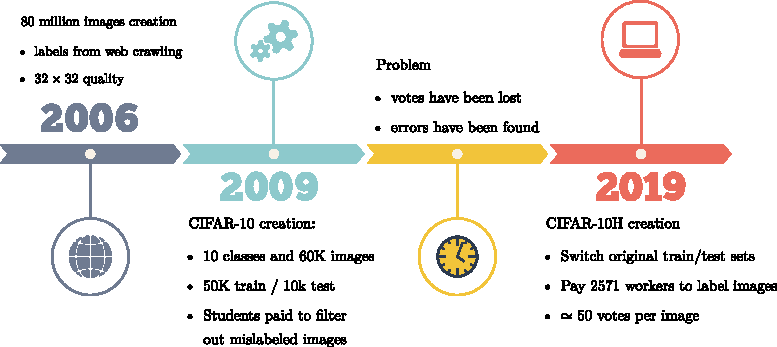
\includegraphics[width=.75\textwidth]{./images/cifar-10h_creation.pdf}
    \end{center}
    Labels: cat, dog, car, plane, bird, horse, frog, deer, ship, truck
    %%%%%%%%%%%%%%%%%%%%%%%%%%%%%%%%%%%%%%%%%%%%%%%%%%%%%%%%%%%%%%%%%%%%%%%%%%%%%%%
    \pause
    \begin{columns}
        \begin{column}{.3\textwidth}
            \    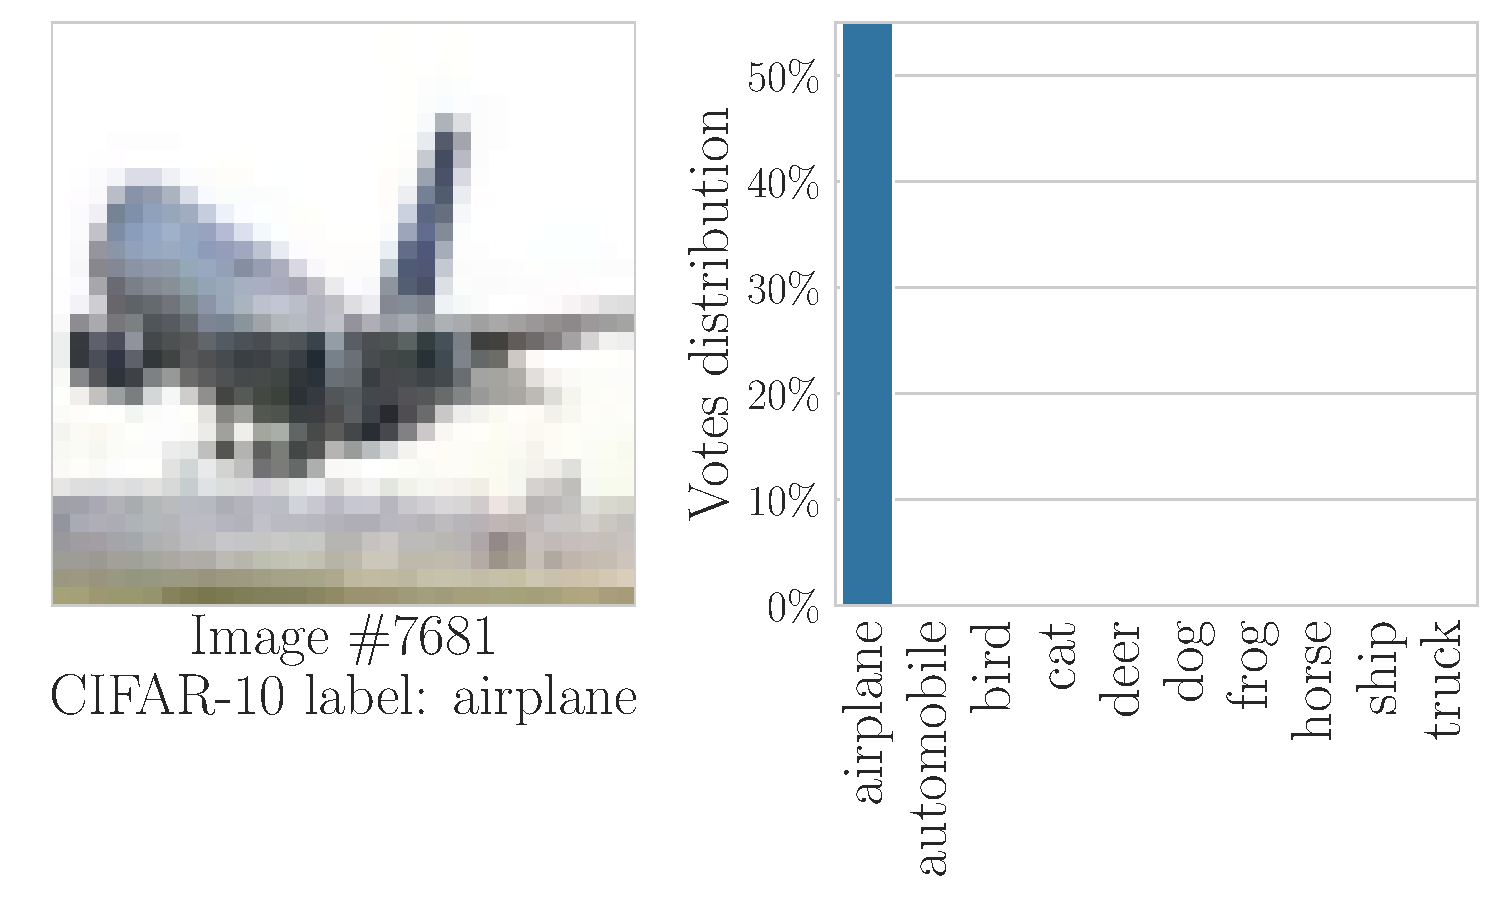
\includegraphics[width=\textwidth]{../chapters/images/image_n_hist7681_paper.pdf}
        \end{column}
        \begin{column}{.3\textwidth}
            \    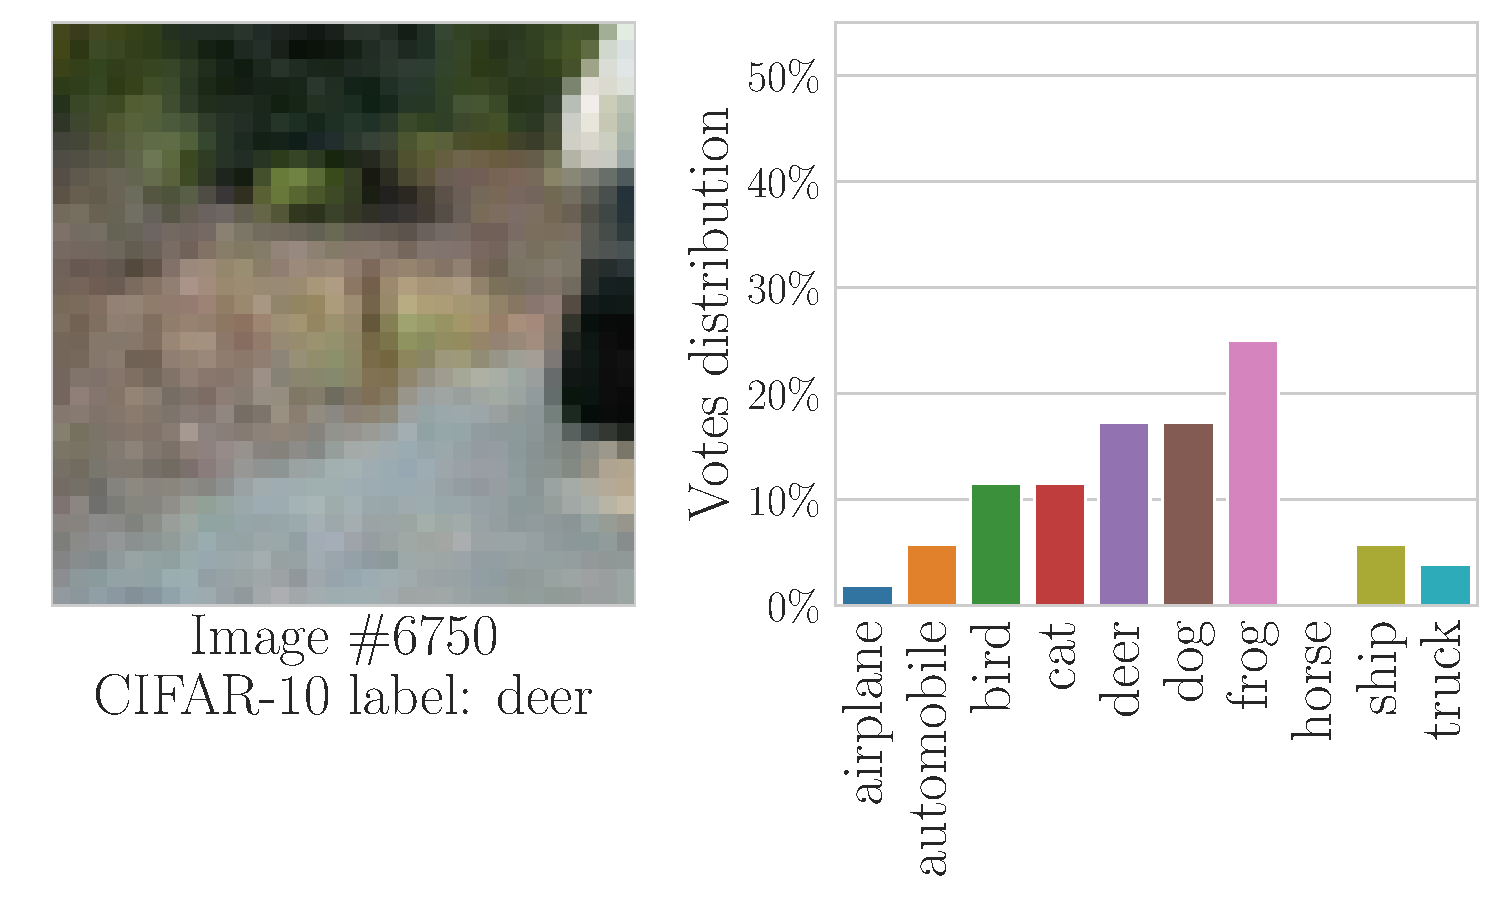
\includegraphics[width=\textwidth]{../chapters/images/image_n_hist6750_paper.pdf}

        \end{column}
        \begin{column}{.3\textwidth}

            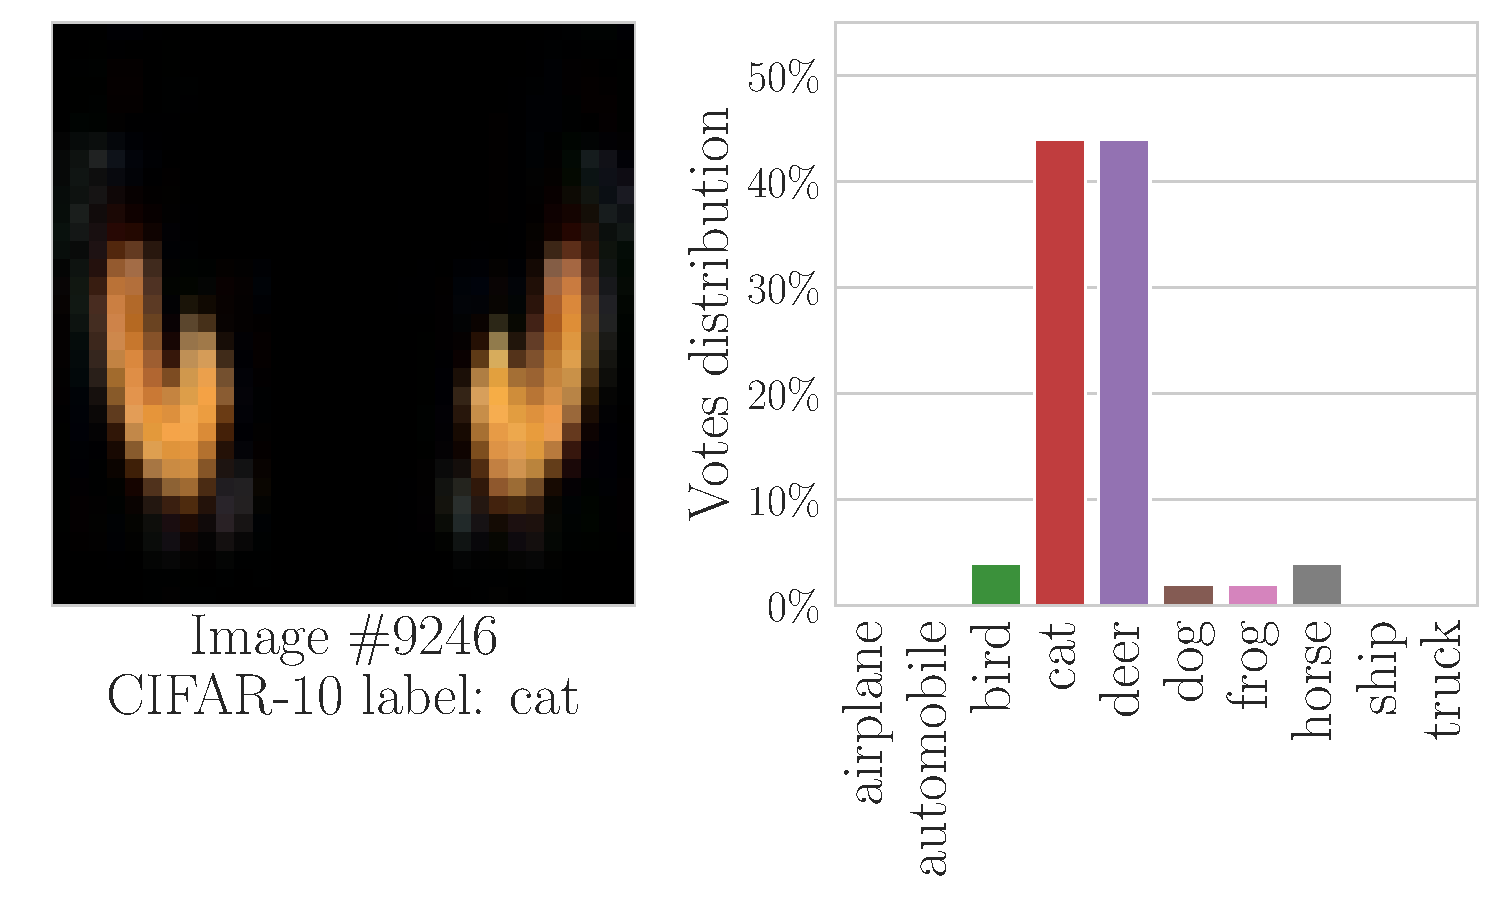
\includegraphics[width=\textwidth]{../chapters/images/image_n_hist9246_paper.pdf}

        \end{column}


    \end{columns}
\end{frame}
%%%%%%%%%%%%%%%%%%%%%%%%%%%%%%%%%%%%%%%%%%%%%%%%%%%%%%%%%%%%%%%%%%%%%%%%%%%%%%%
\begin{frame}{Presenting LabelMe dataset\footfullcite{rodrigues2014gaussian}}{}
\begin{itemize}
    \item 1000 training / 500 validation / 1188 test images
    \item 59 workers: each task has up to 3 votes
    \item 8 classes: highway, insidecity, tallbuilding, street, forest, coast, mountain, opencountry
\end{itemize}

\pause

\centering
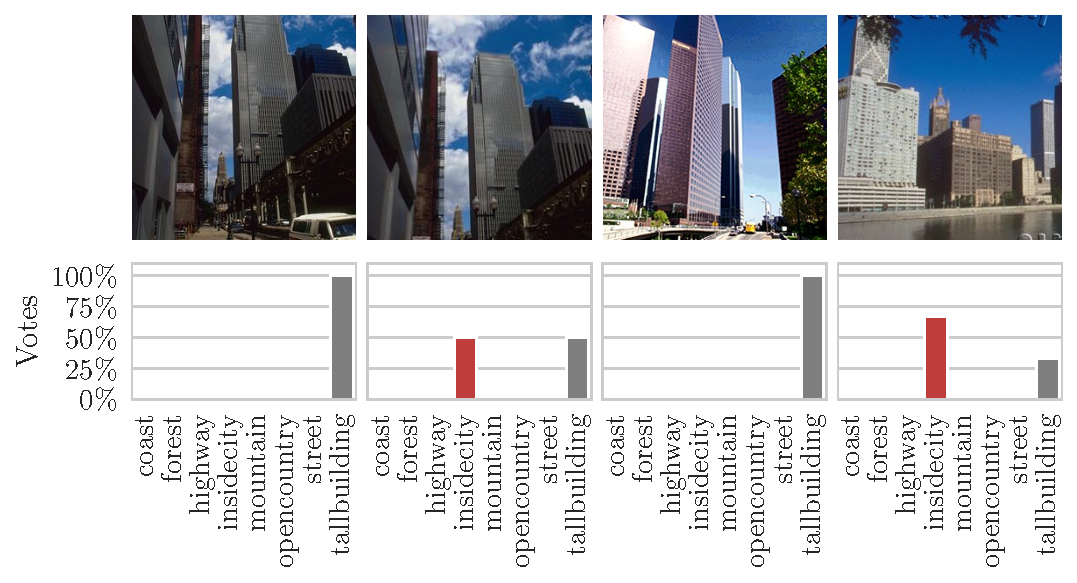
\includegraphics[width=.85\textwidth]{../chapters/images/tallbuilding_and_distrib.pdf}

\end{frame}
%%%%%%%%%%%%%%%%%%%%%%%%%%%%%%%%%%%%%%%%%%%%%%%%%%%%%%%%%%%%%%%%%%%%%%%%%%%%%%%

% %%%%%%%%%%%%%%%%%%%%%%%%%%%%%%%%%%%%%%%%%%%%%%%%%%%%%%%%%%%%%%%%%%%%%%%%%%%%%%%
% \begin{frame}{And the entropy?}{Data sparsity}

% \end{frame}
% %%%%%%%%%%%%%%%%%%%%%%%%%%%%%%%%%%%%%%%%%%%%%%%%%%%%%%%%%%%%%%%%%%%%%%%%%%%%%%%

%%%%%%%%%%%%%%%%%%%%%%%%%%%%%%%%%%%%%%%%%%%%%%%%%%%%%%%%%%%%%%%%%%%%%%%

%%%%%%%%%%%%%%%%%%%%%%%%%%%%%%%%%%%%%%%%%%%%%%%%%%%%%%%%%%%%%%%%%%%%%%%%%%%%%%%%%%%%%%%%%%%%%%%%
\begin{frame}{Qualitative results}{}
    \begin{columns}
    \begin{column}{.3\textwidth}
        \textbf{WAUM}

        (crowdsourcing)

        \vspace{.25cm}

        \centering
           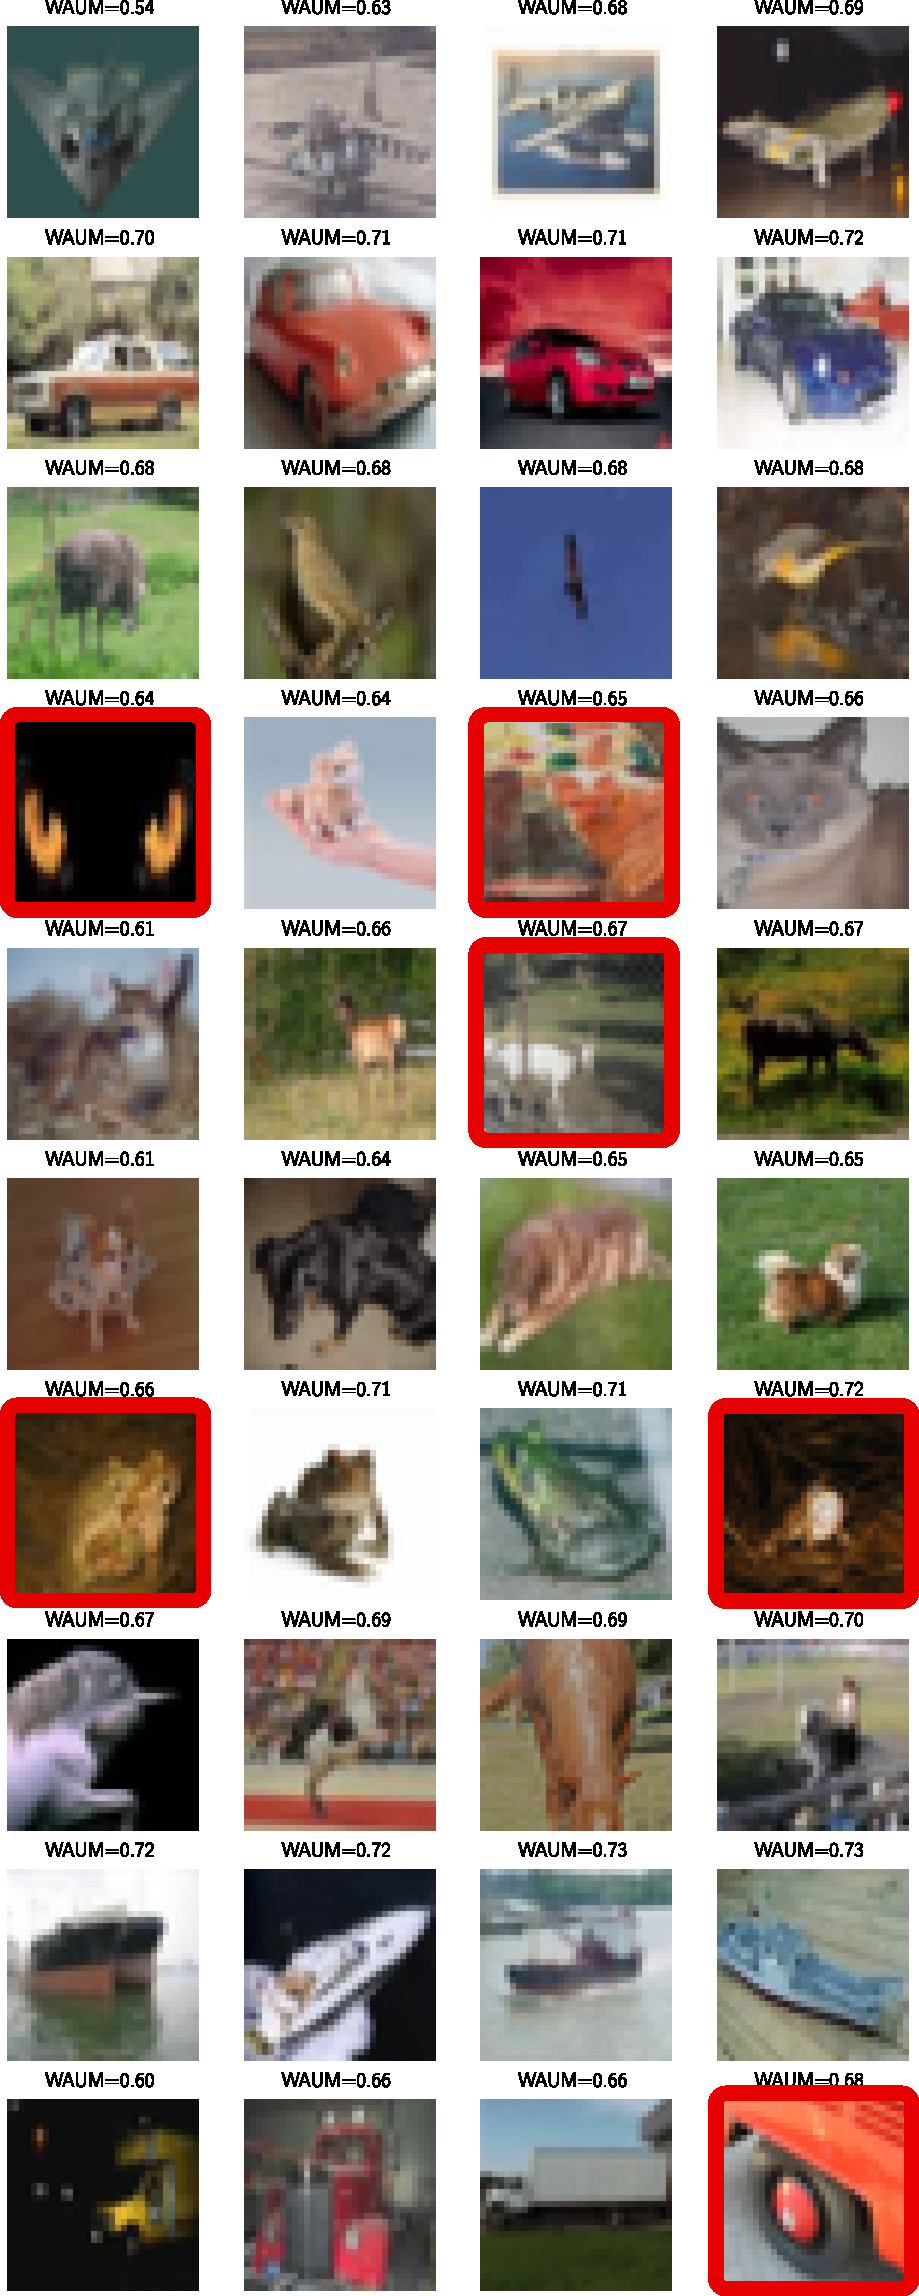
\includegraphics[width=\textwidth, clip, trim={0cm 0cm 0cm 12cm}]{../chapters/images/lowest_waums_cut.pdf}

        \end{column}

        \begin{column}{.3\textwidth}
            \textbf{AUMC}

            (crowdsourcing)

            \vspace{.25cm}

            \centering
               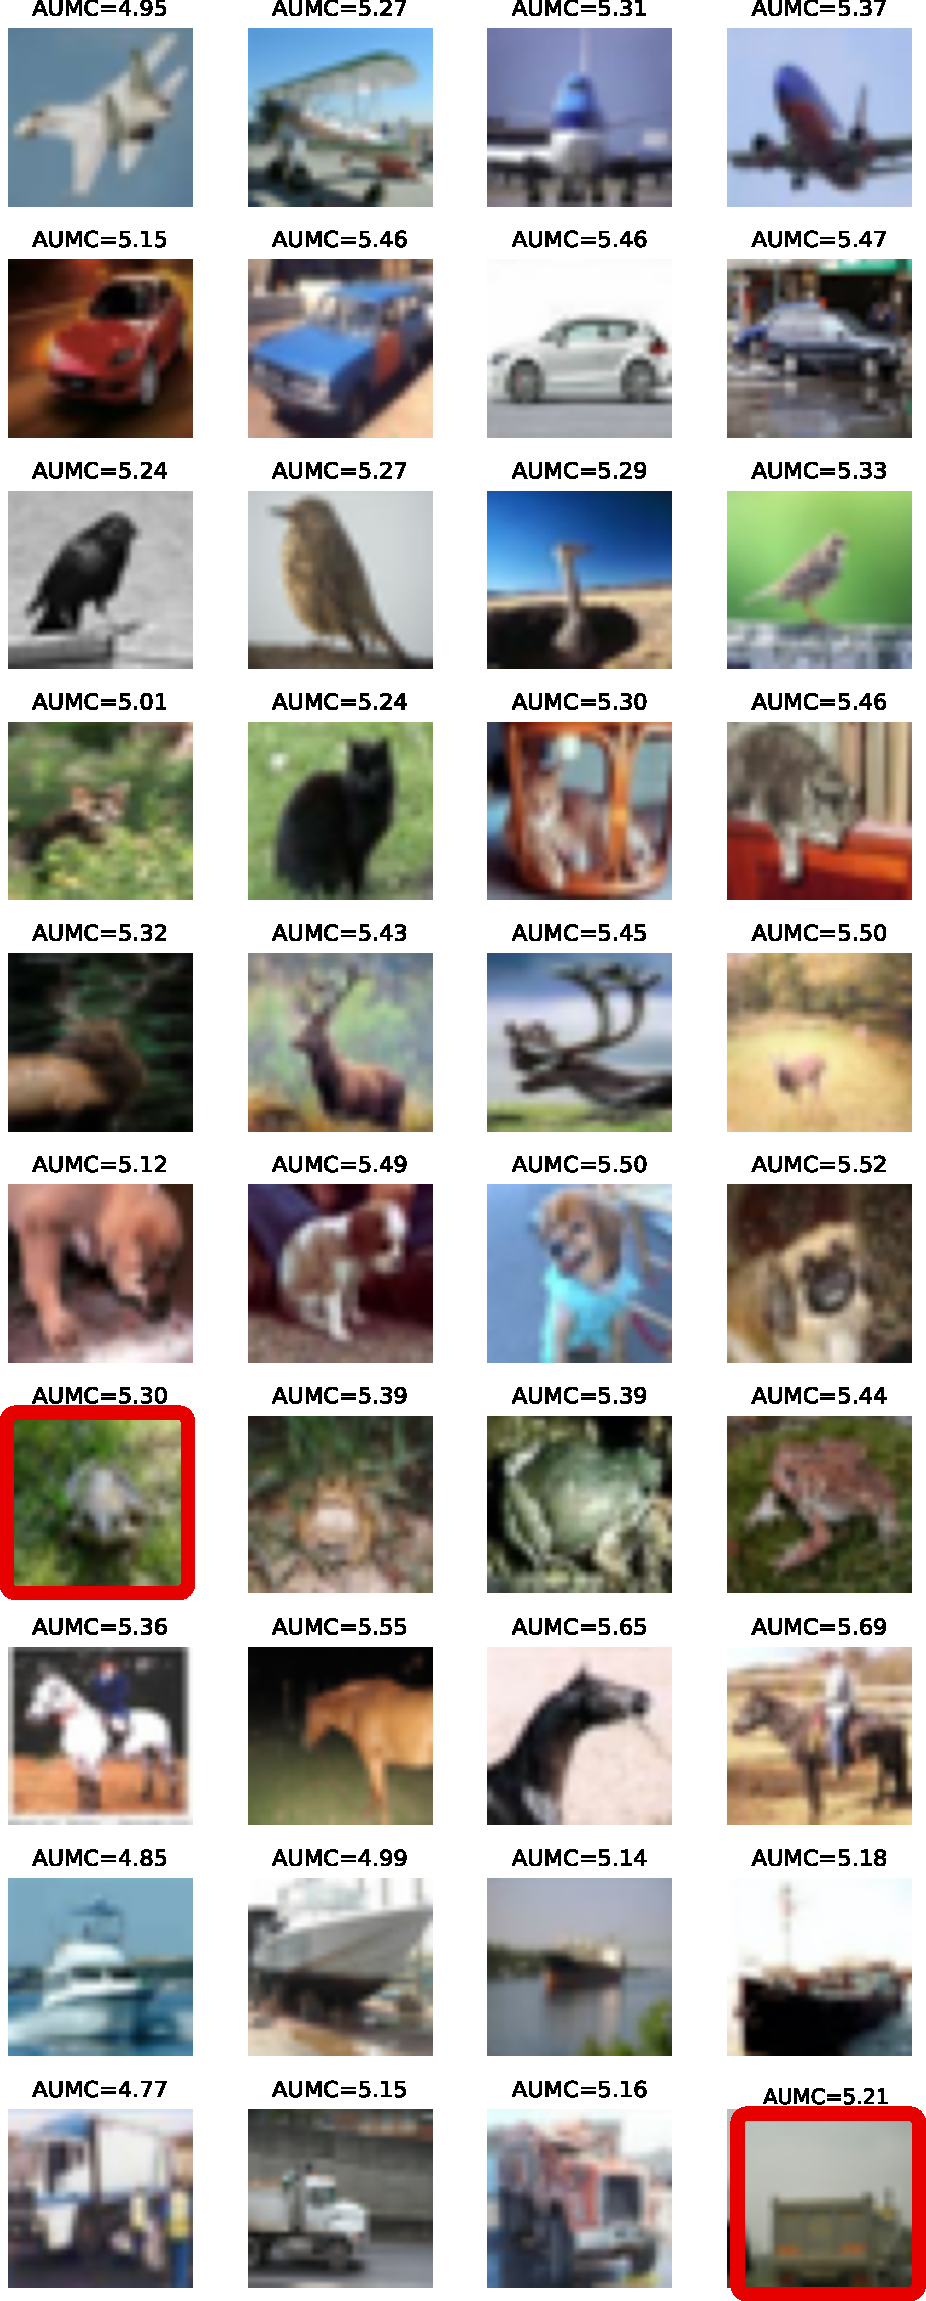
\includegraphics[width=\textwidth, clip, trim={0cm 0cm 0cm 12cm}]{../chapters/images/AUMC_yang_cut.pdf}
        \end{column}
        \begin{column}{.3\textwidth}
            \textbf{AUM}

            (no crowdsourcing)

            \vspace{.25cm}

            \centering
            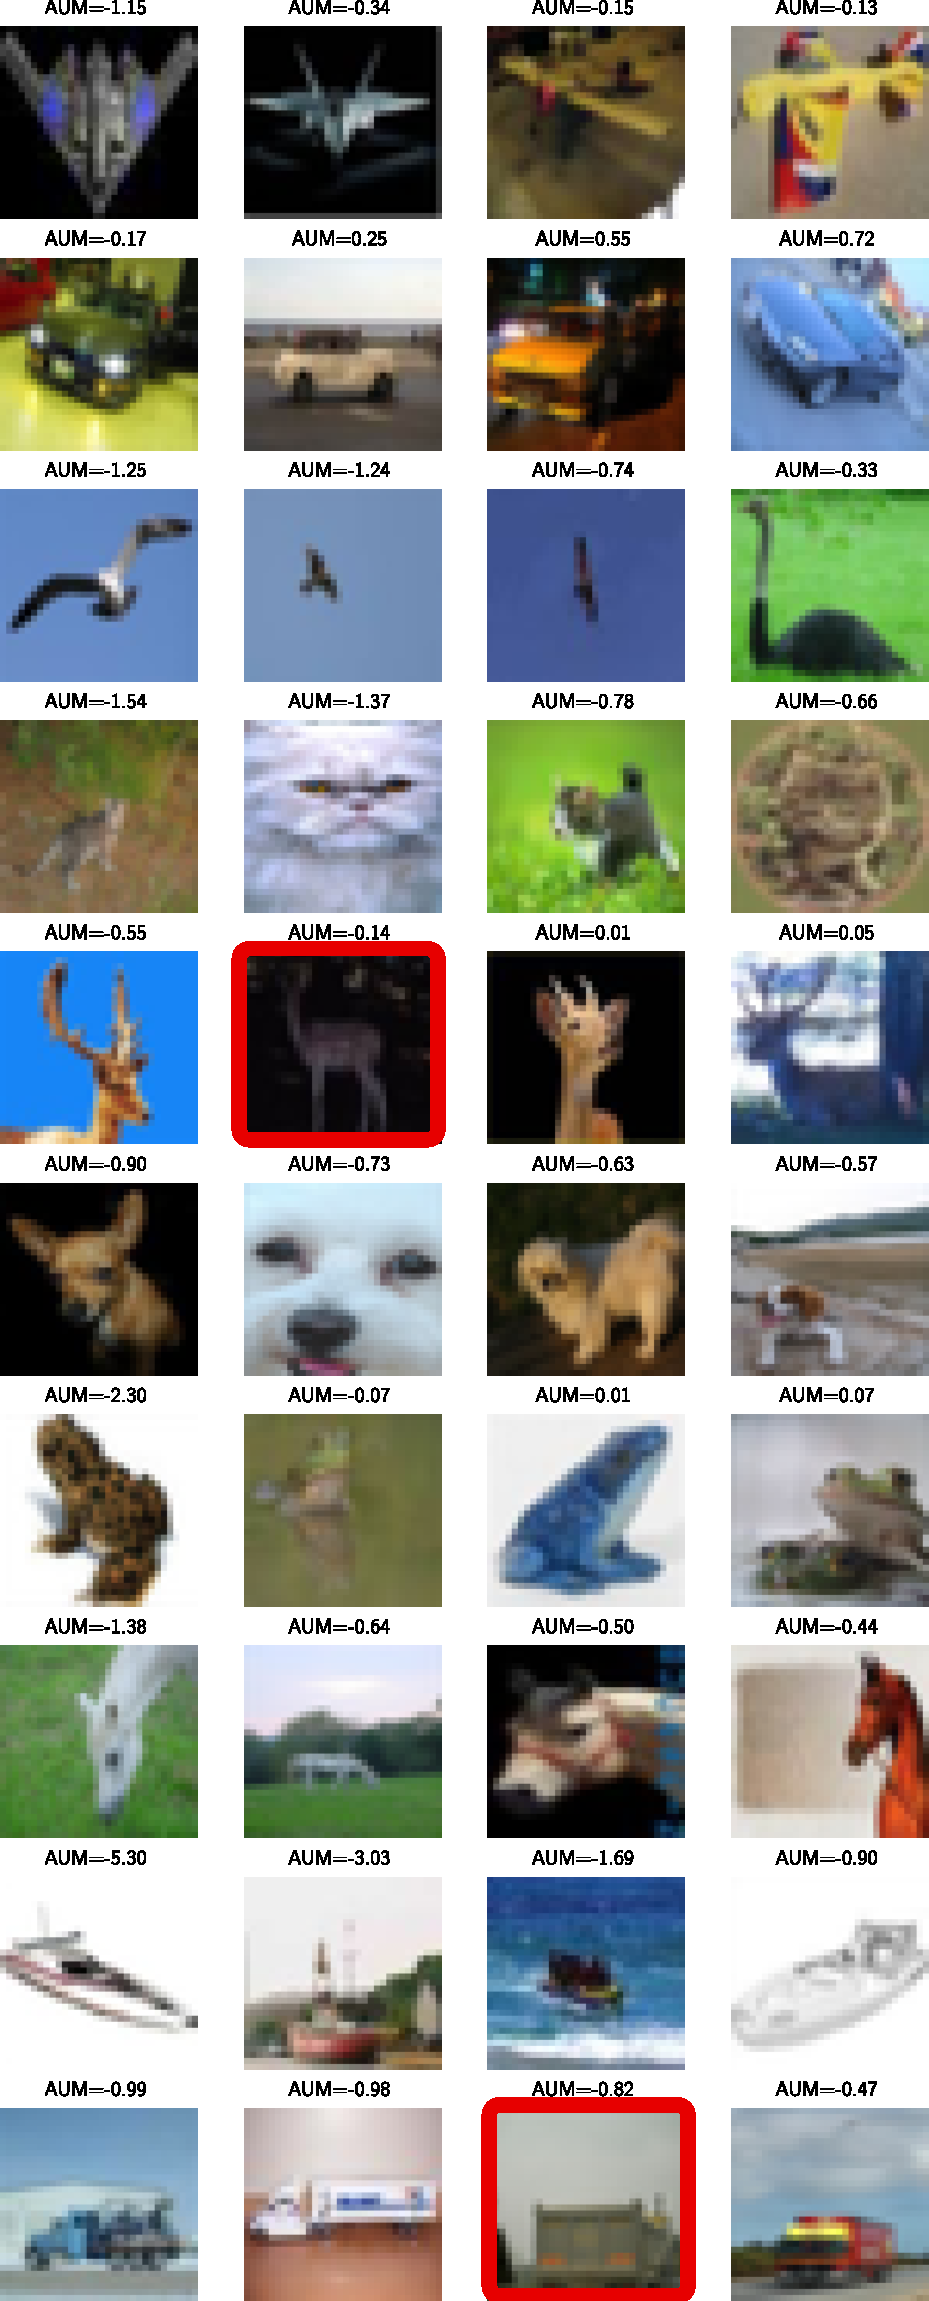
\includegraphics[width=\textwidth, clip, trim={0cm 0cm 0cm 12cm}]{../chapters/images/lowest_aum_cut.pdf}
        \end{column}

    \end{columns}

\end{frame}
%%%%%%%%%%%%%%%%%%%%%%%%%%%%%%%%%%%%%%%%%%%%%%%%%%%%%%%%%%%%%%%%%%%%%%%%%%%%%%%

%%%%%%%%%%%%%%%%%%%%%%%%%%%%%%%%%%%%%%%%%%%%%%%%%%%%%%%%%%%%%%%%%%%%%%%%%%%%%%%
\begin{frame}{Ablation study}{}
    \begin{columns}
        \begin{column}{.5\textwidth}
            \textbf{CIFAR-10H}

            \vspace{.25cm}

            \centering
               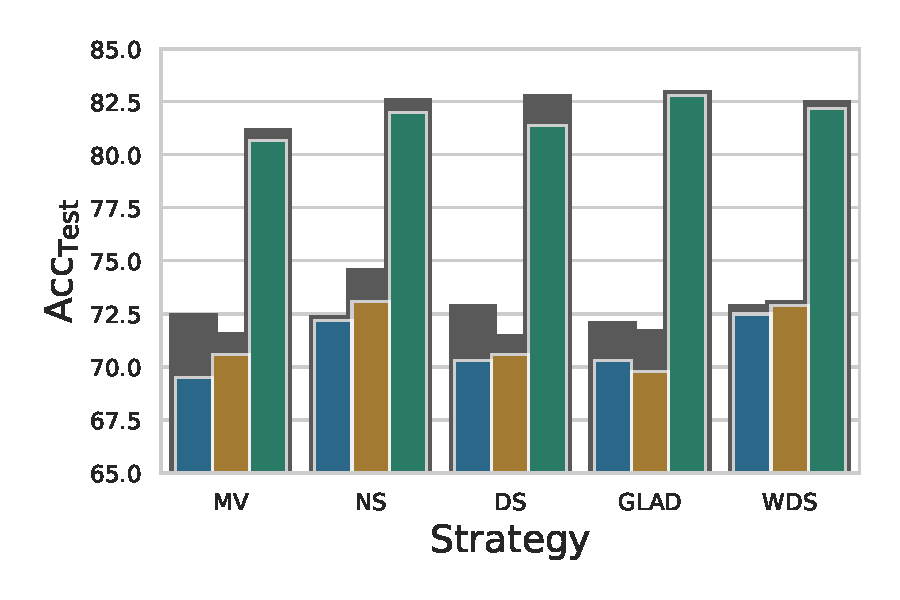
\includegraphics[width=\textwidth]{../chapters/images/acc_cifar10H.pdf}

            \end{column}

            \begin{column}{.5\textwidth}
                \textbf{LabelMe}

                \vspace{.25cm}

                \centering
                   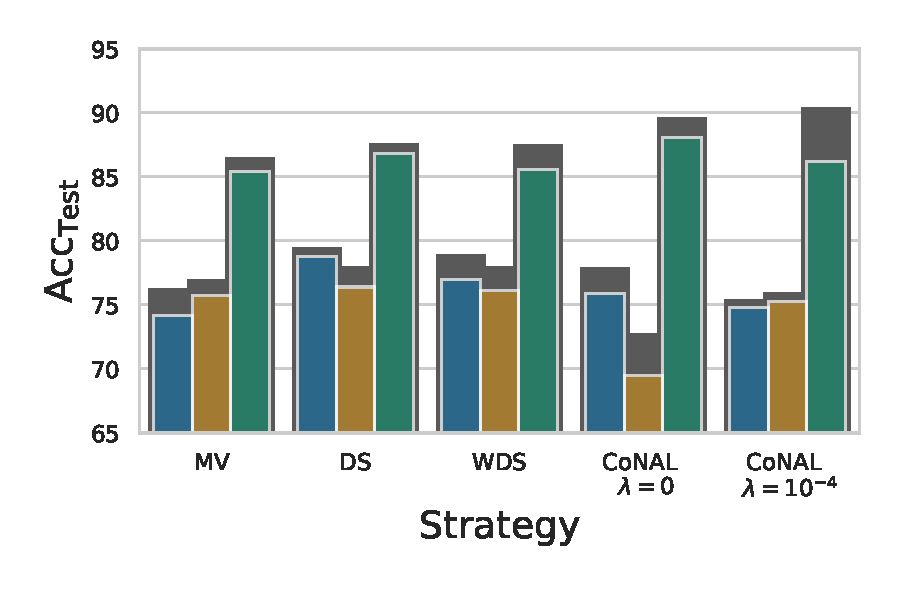
\includegraphics[width=\textwidth]{../chapters/images/acc_labelme.pdf}
            \end{column}

        \end{columns}
    \centering
    
\includegraphics[width=.75\textwidth]{../chapters/images/legend_ablation_study.pdf}
\end{frame}
%%%%%%%%%%%%%%%%%%%%%%%%%%%%%%%%%%%%%%%%%%%%%%%%%%%%%%%%%%%%%%

%%%%%%%%%%%%%%%%%%%%%%%%%%%%%%%%%%%%%%%%%%%%%%%%%%%%%%%%%%%%%%%%%%%%%%%%%%%%%%%
\begin{frame}{Discussion}{Going to the large-scale problem}
\begin{block}{In short}
\begin{itemize}
    \item Introduced the WAUM to find ambiguous images
    \item Better quality data can improve performance
\end{itemize}
\end{block}

\pause
\begin{block}{Towards large-scale problems}
\begin{itemize}
    \item DS model and confusion matrices do not scale
    \item What is currently done in large-scale settings?
    \item Can we evaluate their performance?
    \begin{itemize}
    \item<3> \textcolor{red}{To evaluate we need data and code that scale!}
    \end{itemize}
\end{itemize}
\end{block}
\end{frame}
%%%%%%%%%%%%%%%%%%%%%%%%%%%%%%%%%%%%%%%%%%%%%%%%%%%%%%%%%%%%%%%%%%%%%%%%%%%%%%%

\section{The peerannot library}

\begin{frame}{Peerannot library}{Handle crowdsourced data in classification}
    \begin{itemize}
        \item Python library for small and large crowdsourced datasets \\
        \begin{center} \texttt{pip install peerannot}\end{center}
        \item Documentation available at: \url{https://peerannot.github.io}
    \end{itemize}
    \begin{center}
        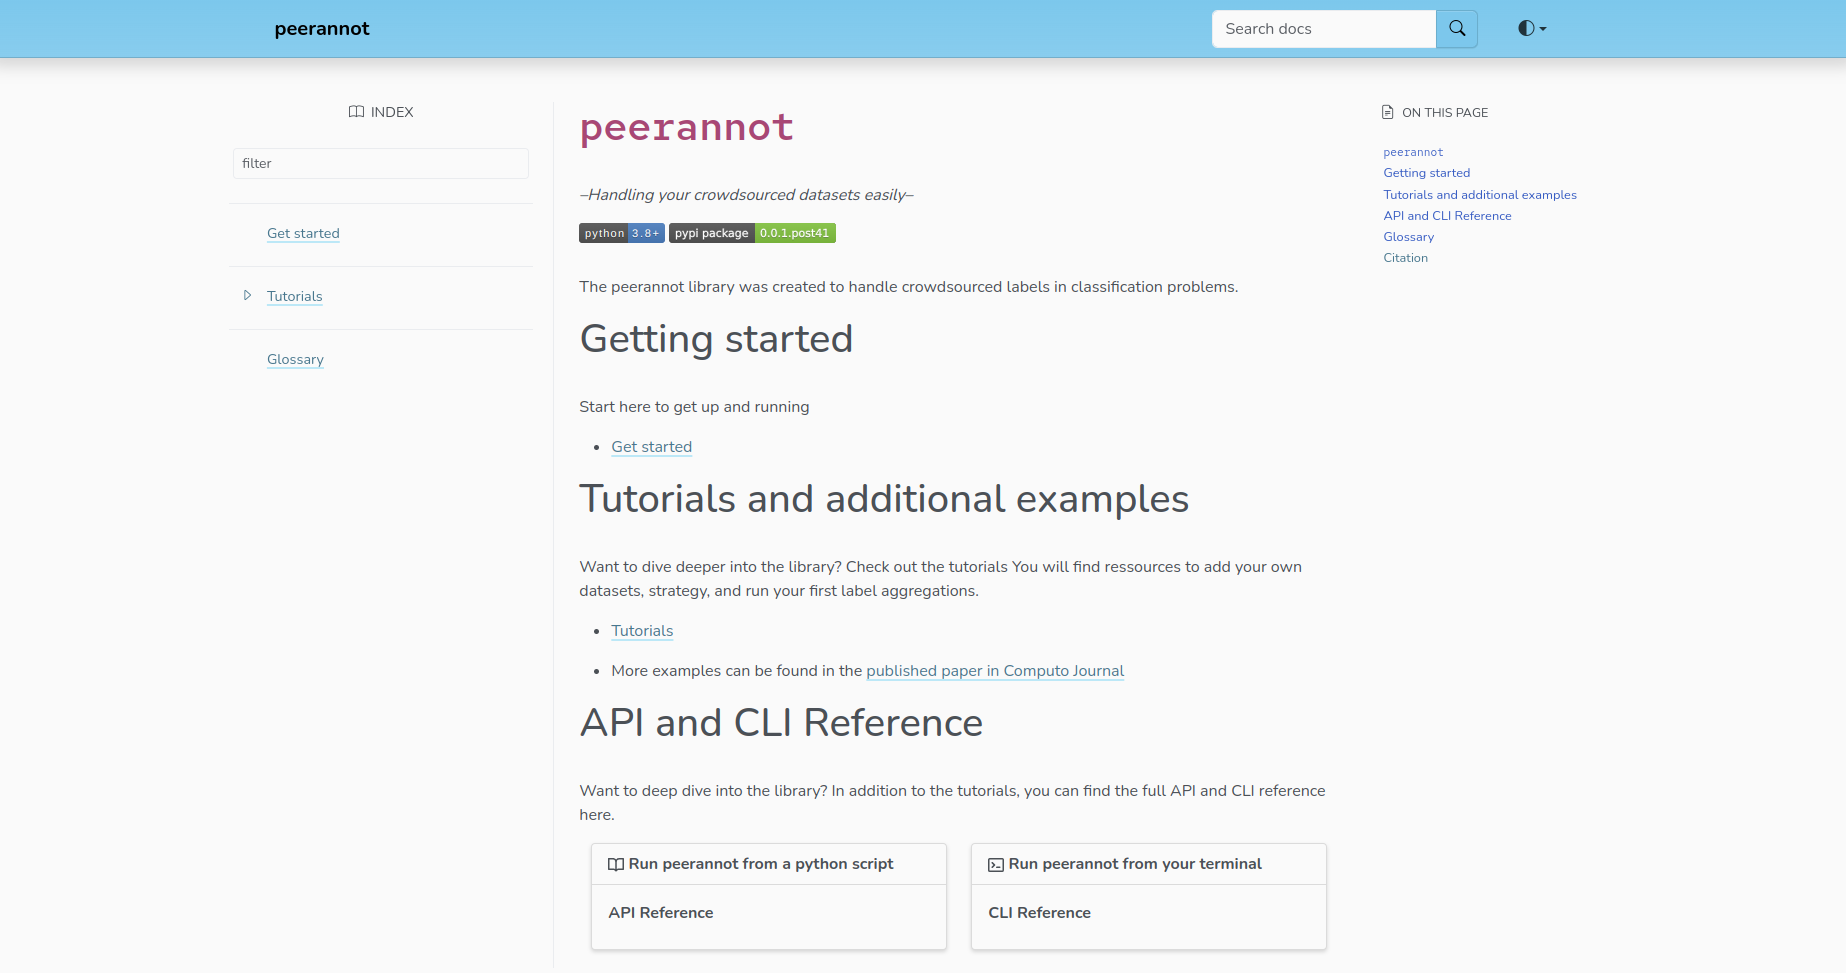
\includegraphics[width=\textwidth]{./images/peerannot_web.png}
    \end{center}
\end{frame}

\section{Crowdsourcing in large scale: the case of Pl@ntNet}

%%%%%%%%%%%%%%%%%%%%%%%%%%%%%%%%%%%%%%%%%%%%%%%%%%%%%%%%%%%%%%%%%%%%%%%%%%%%%%%
\begin{frame}{Presenting Pl@ntNet pipeline}
\begin{center}
    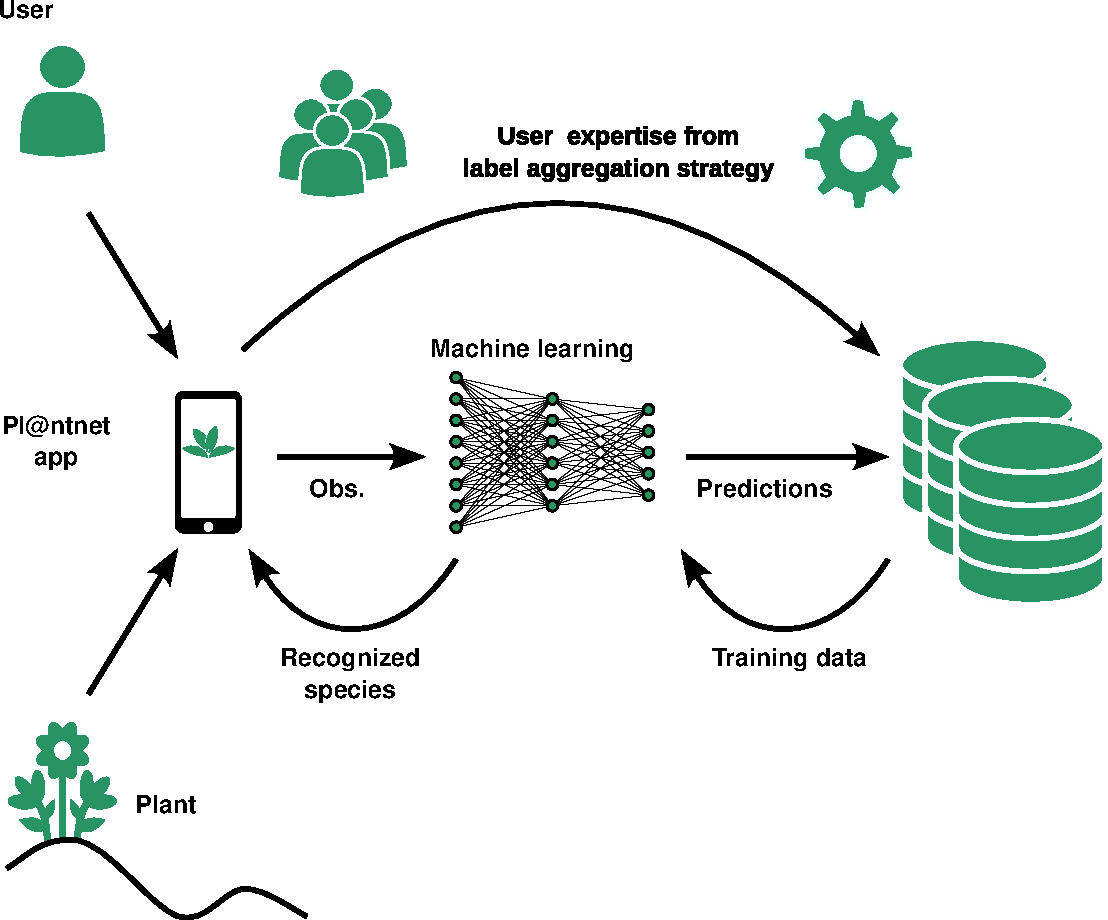
\includegraphics[width=.85\textwidth]{../chapters/images/plantnet_schema_global_green.pdf}
\end{center}
\end{frame}
%%%%%%%%%%%%%%%%%%%%%%%%%%%%%%%%%%%%%%%%%%%%%%%%%%%%%%%%%%%%%%%%%%%%%%%%%%%%%%%
%%%%%%%%%%%%%%%%%%%%%%%%%%%%%%%%%%%%%%%%%%%%%%%%%%%%%%%%%%%%%%%%%%%%%%%%%%%%%%%
\begin{frame}{Realeasing a new dataset}{}
    \begin{itemize}
        \item South Western European flora obs since $2017$
        \item $n_{\text{worker}}\simeq 823\ 000$ users answered more than $K\simeq 11 000$ species
        \item $n_{\text{task}}\simeq 6\ 700\ 000$ observations
        \item $9\ 000\ 000$ votes casted
        \item \textbf{Imbalance}: 80\% of observations are represented by 10\% of total votes
    \end{itemize}
\pause
\vspace{1cm}
\begin{itemize}
    \item Extraction of $98$ experts (TelaBotanica + expert knowledge)
    \vspace{1cm}
    \item \url{https://zenodo.org/records/10782465}
\end{itemize}
\end{frame}
%%%%%%%%%%%%%%%%%%%%%%%%%%%%%%%%%%%%%%%%%%%%%%%%%%%%%%%%%%%%%%%%%%%%%%%%%%%%%%%

%%%%%%%%%%%%%%%%%%%%%%%%%%%%%%%%%%%%%%%%%%%%%%%%%%%%%%%%%%%%%%%%%%%%%%%%%%%%%%%
\begin{frame}{Pl@ntNet aggregation strategy}
    \begin{center}
        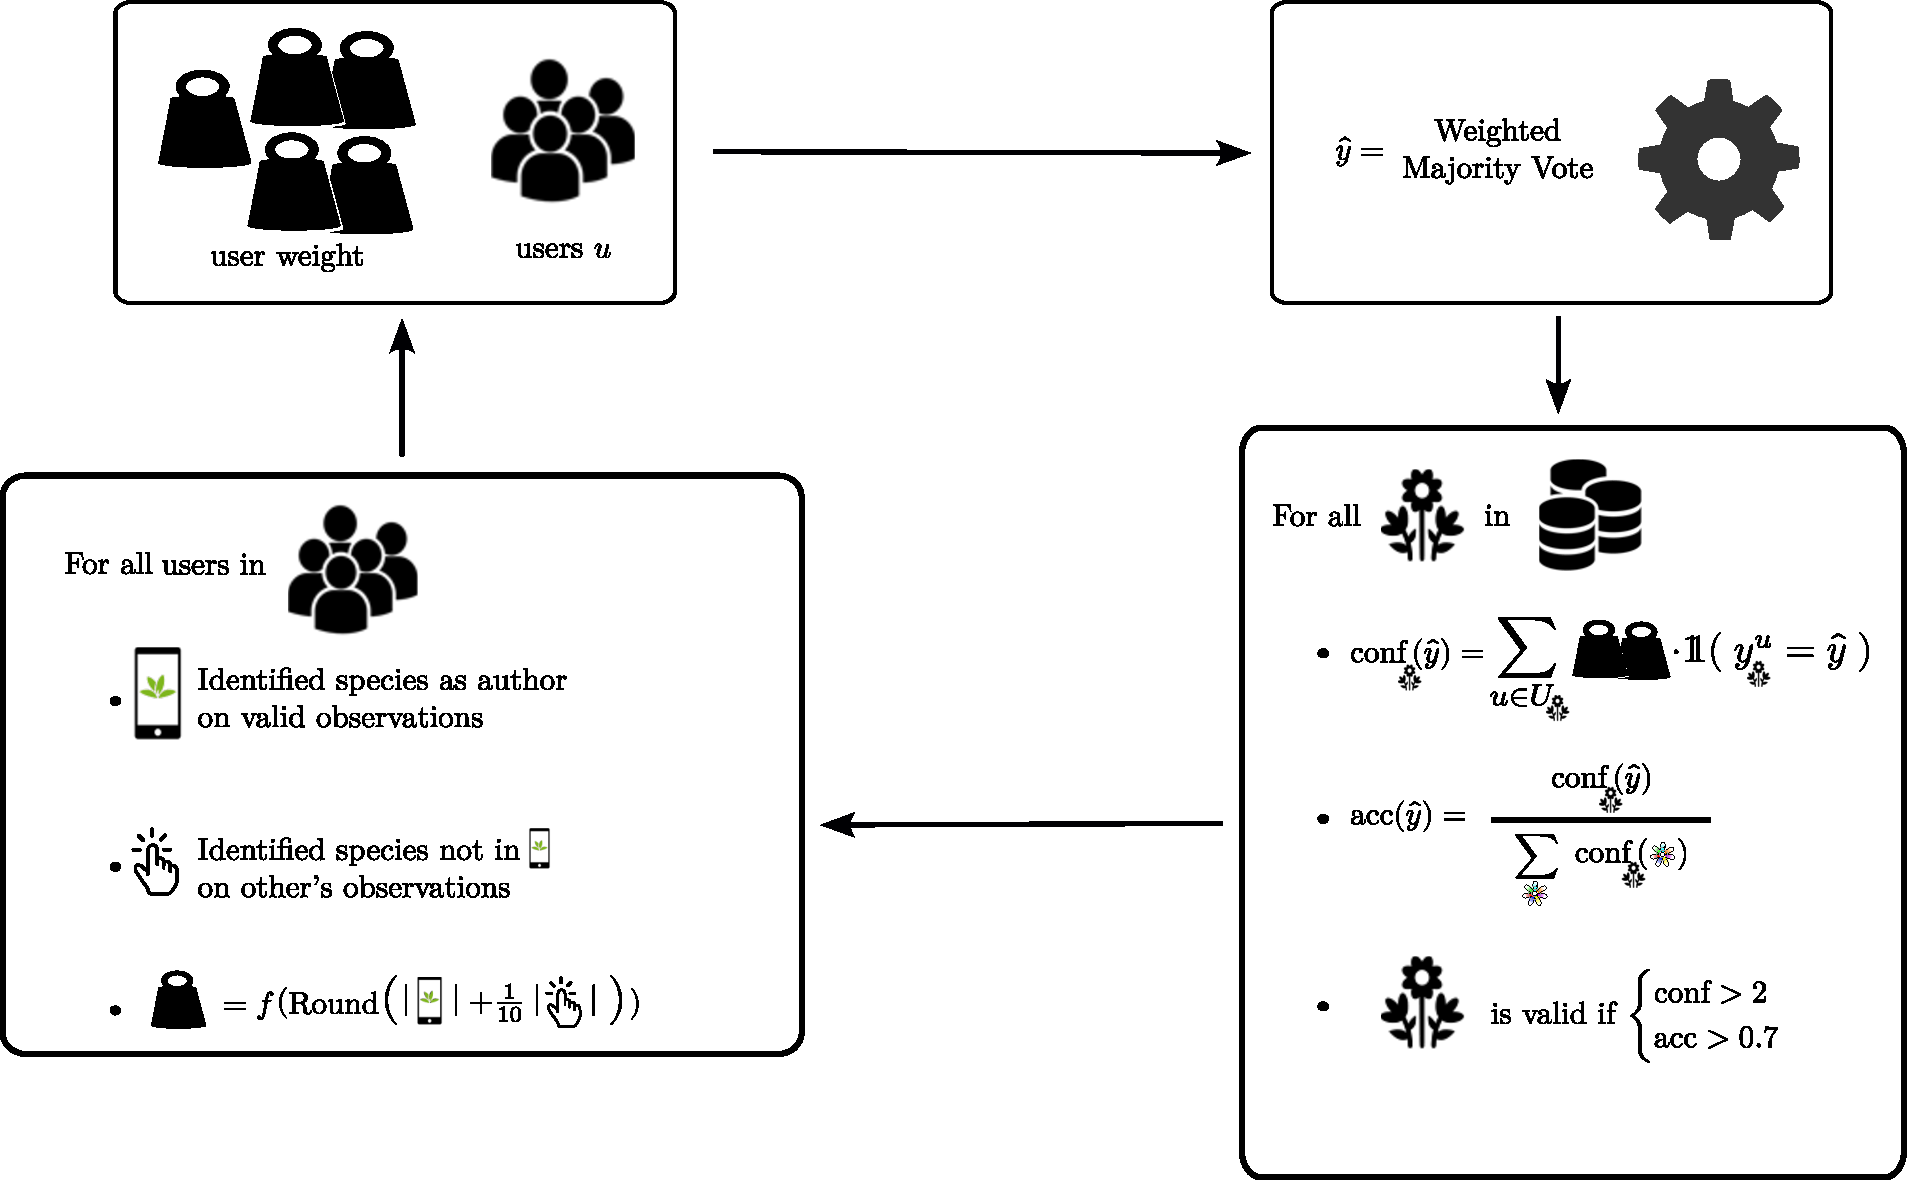
\includegraphics[width=\textwidth]{../chapters/images_plantnet/schema_plantnet_aggregation.pdf}
    \end{center}
\end{frame}
%%%%%%%%%%%%%%%%%%%%%%%%%%%%%%%%%%%%%%%%%%%%%%%%%%%%%%%%%%%%%%%%%%%%%%%%%%%%%%%

%%%%%%%%%%%%%%%%%%%%%%%%%%%%%%%%%%%%%%%%%%%%%%%%%%%%%%%%%%%%%%%%%%%%%%%%%%%%%%%
% \begin{frame}{Pl@ntNet aggregation strategy}{Weight function}
% \[f(n_j)=n_j^\alpha -n_j^\beta + \gamma \text{ with }\begin{cases} \alpha&=0.5 \\ \beta &=0.2 \\ \gamma&\simeq 0.74\end{cases}\]

% \begin{center}
%     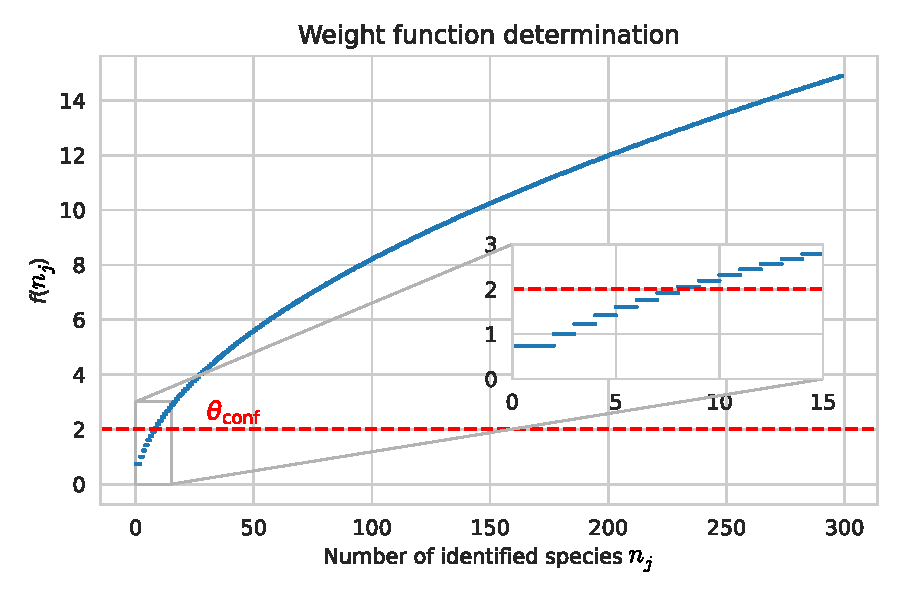
\includegraphics[width=.6\textwidth]{../chapters/images_plantnet/weight_function.pdf}
% \end{center}

% \begin{itemize}
%     \item With 8 identified species one becomes self-validating
%     \item<2> But observations can be invalidated at any time in the future
% \end{itemize}
% \end{frame}
% %%%%%%%%%%%%%%%%%%%%%%%%%%%%%%%%%%%%%%%%%%%%%%%%%%%%%%%%%%%%%%%%%%%%%%%%%%%%%%%

%%%%%%%%%%%%%%%%%%%%%%%%%%%%%%%%%%%%%%%%%%%%%%%%%%%%%%%%%%%%%%%%%%%%%%%%%%%%%%%
\begin{frame}{Pl@ntNet aggregation strategy}{Examples}
    \begin{onlyenv}<1>
        Initial setting
        \begin{columns}
            \begin{column}{.5\textwidth}
                \begin{center}
                    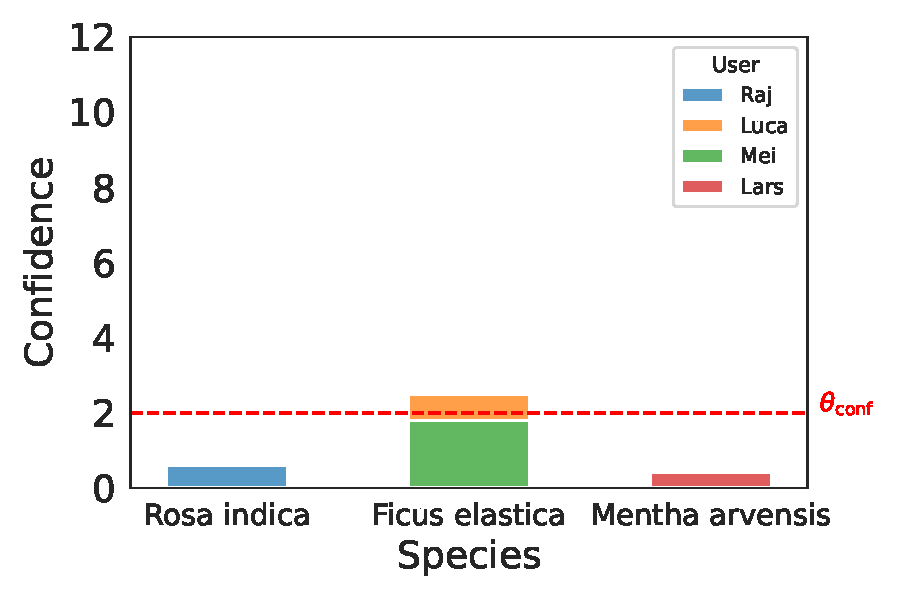
\includegraphics[width=\textwidth]{./images/histplot_conf_init.pdf}
                \end{center}
            \end{column}
            \begin{column}{.5\textwidth}
                \begin{center}
                    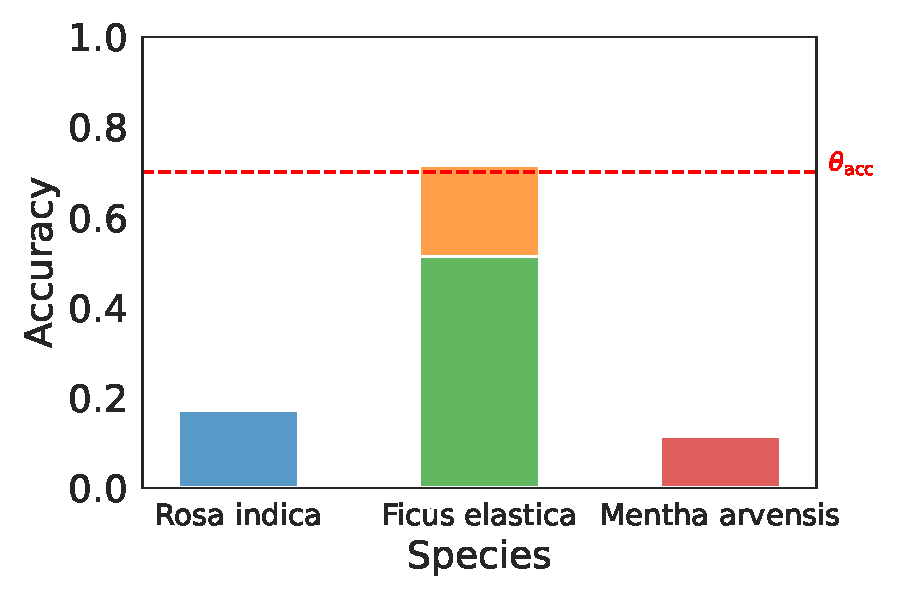
\includegraphics[width=\textwidth]{./images/histplot_acc_init.pdf}
                \end{center}
            \end{column}
        \end{columns}
    \end{onlyenv}
    \begin{onlyenv}<2>
        Label switch\phantom{g}
        \begin{columns}
            \begin{column}{.5\textwidth}
                \begin{center}
                    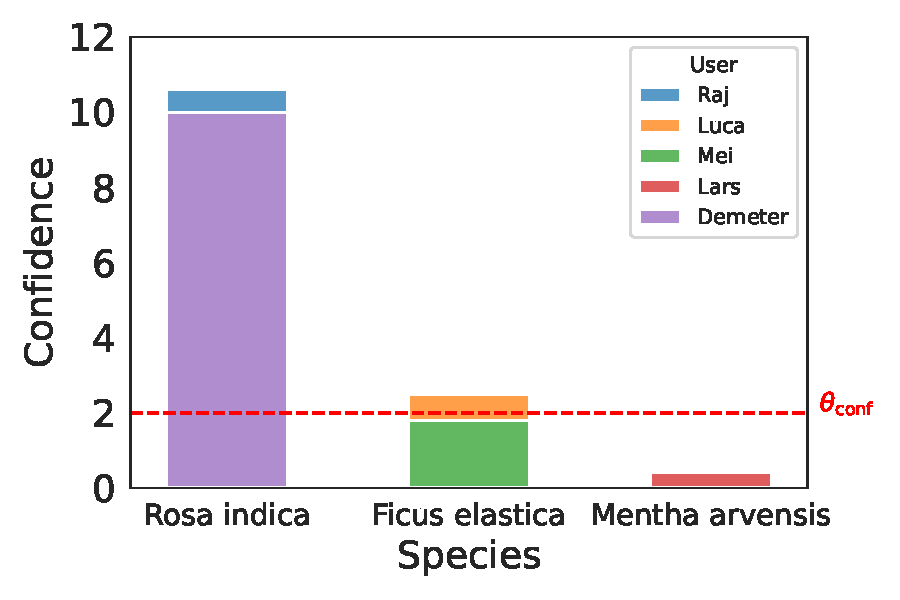
\includegraphics[width=\textwidth]{./images/histplot_conf_switch.pdf}
                \end{center}
            \end{column}
            \begin{column}{.5\textwidth}
                \begin{center}
                    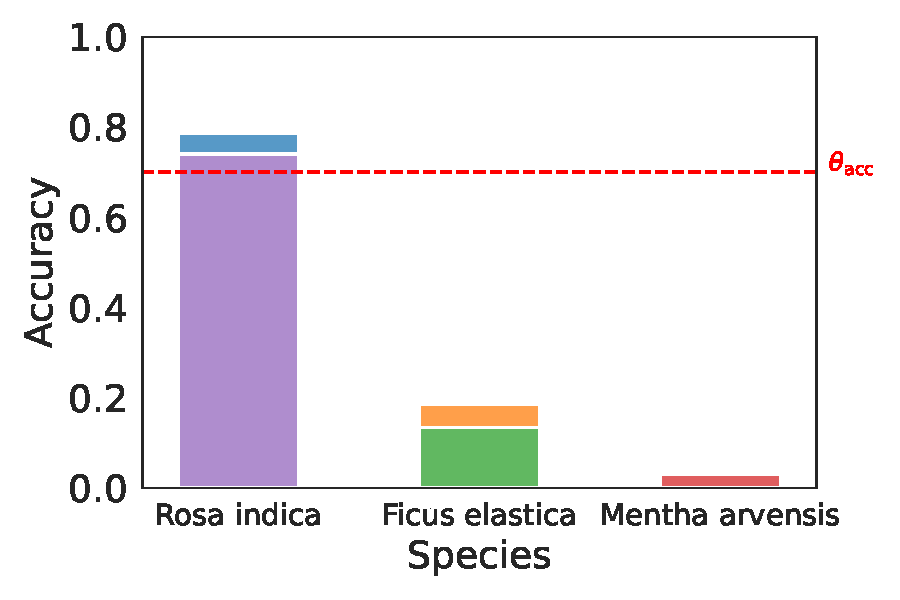
\includegraphics[width=\textwidth]{./images/histplot_acc_switch.pdf}
                \end{center}
            \end{column}
        \end{columns}
    \end{onlyenv}
    \begin{onlyenv}<3>
        Invalidate\phantom{g}
        \begin{columns}
            \begin{column}{.5\textwidth}
                \begin{center}
                    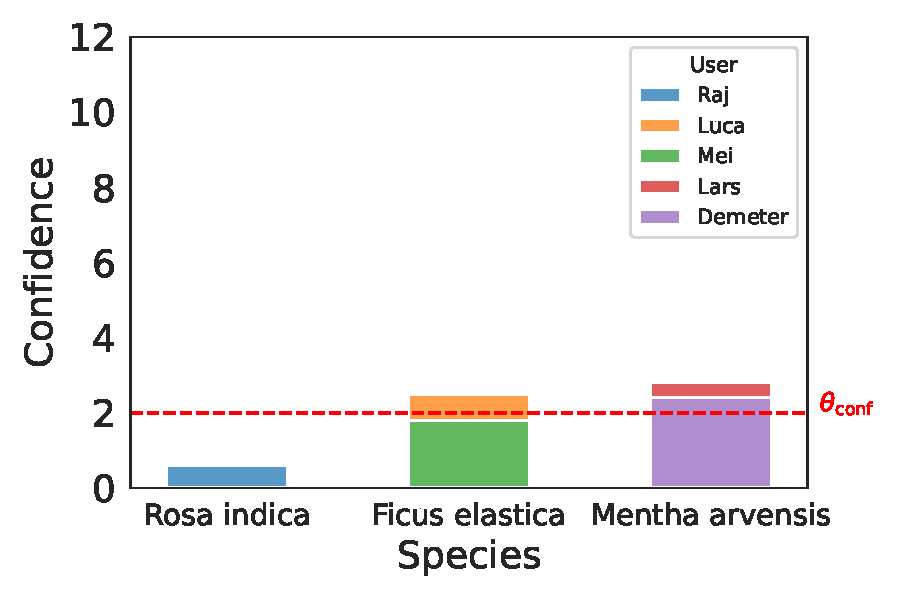
\includegraphics[width=\textwidth]{./images/histplot_conf_invalidate.pdf}
                \end{center}
            \end{column}
            \begin{column}{.5\textwidth}
                \begin{center}
                    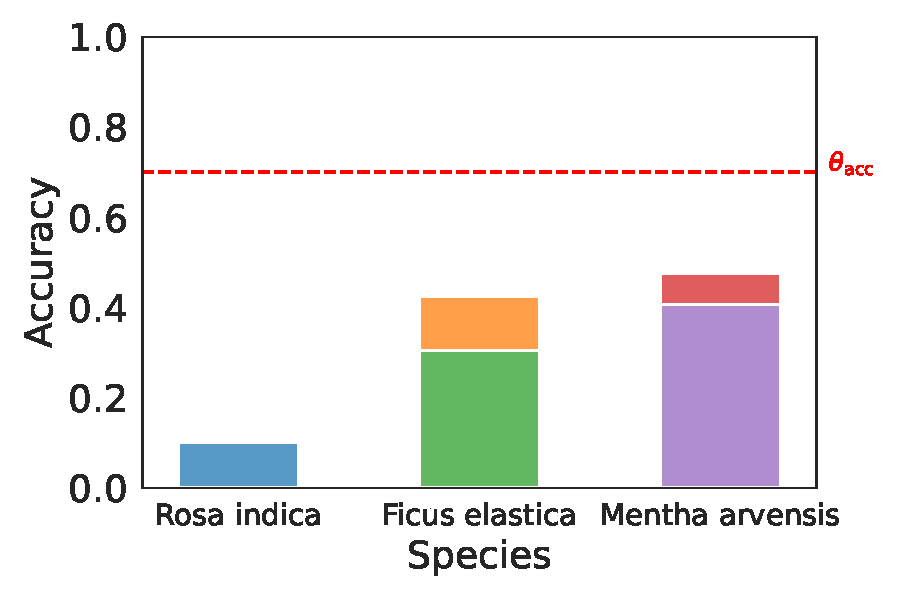
\includegraphics[width=\textwidth]{./images/histplot_acc_invalidate.pdf}
                \end{center}
            \end{column}
        \end{columns}
    \end{onlyenv}
\end{frame}
%%%%%%%%%%%%%%%%%%%%%%%%%%%%%%%%%%%%%%%%%%%%%%%%%%%%%%%%%%%%%%%%%%%%%%%%%%%%%%%

%%%%%%%%%%%%%%%%%%%%%%%%%%%%%%%%%%%%%%%%%%%%%%%%%%%%%%%%%%%%%%%%%%%%%%%%%%%%%%%
\begin{frame}{Compared strategies}{}
    \begin{itemize}
        \item<1-> \textbf{Majority Vote} (MV)
        \item<2-> \textbf{Worker agreement with aggregate (WAWA)}
        \[    \mathrm{weight}(w_j) = \mathrm{Accuracy}(\{y_i^{(j)}\}_i, \{\hat {y_i}^\mathrm{MV}\}_i)
        \]
        \item<3-> \textbf{TwoThird} (from iNaturalist pipeline)
        \begin{itemize}
            \item[$\bullet$] Need 2 votes
            \item[$\bullet$] $2/3$ of agreements
        \end{itemize}
    \end{itemize}
\end{frame}
%%%%%%%%%%%%%%%%%%%%%%%%%%%%%%%%%%%%%%%%%%%%%%%%%%%%%%%%%%%%%%%%%%%%%%%%%%%%%%%

%%%%%%%%%%%%%%%%%%%%%%%%%%%%%%%%%%%%%%%%%%%%%%%%%%%%%%%%%%%%%%%%%%%%%%%%%%%%%%%
\begin{frame}{Results}{}
    \centering
%     \begin{columns}[c]
%    \begin{column}{0.4\textwidth}
%        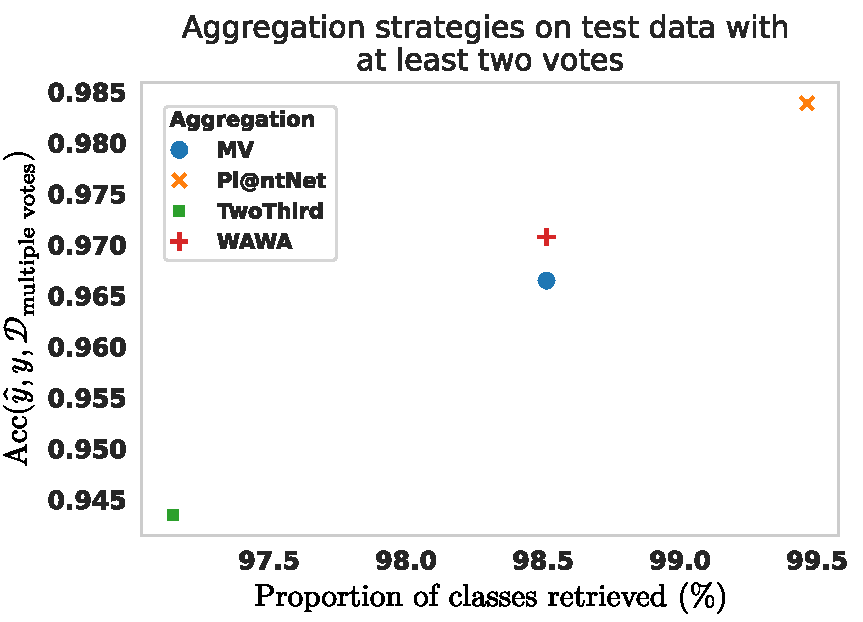
\includegraphics[width=\linewidth, height=3cm]{./images/accuracy_by_vol_class_kept_two_votes__micro-5.pdf}
%            \end{column}
%    \begin{column}{0.4\textwidth}
%        \label{fig:accuracy_vol_class_multiple}
%        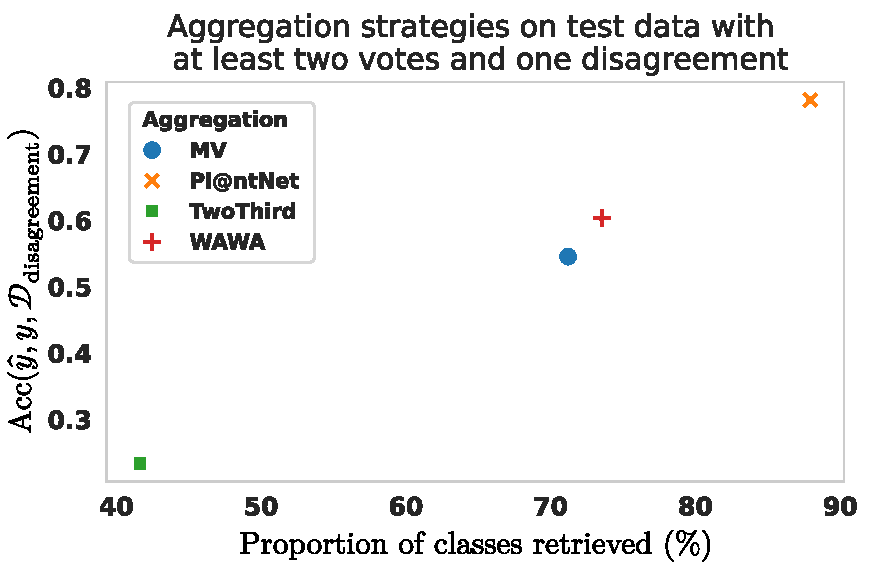
\includegraphics[width=\linewidth, height=3cm]{./images/accuracy_by_vol_class_kept_one_disagreeement__micro-5.pdf}
%            \end{column}
%  \end{columns}
\begin{center}
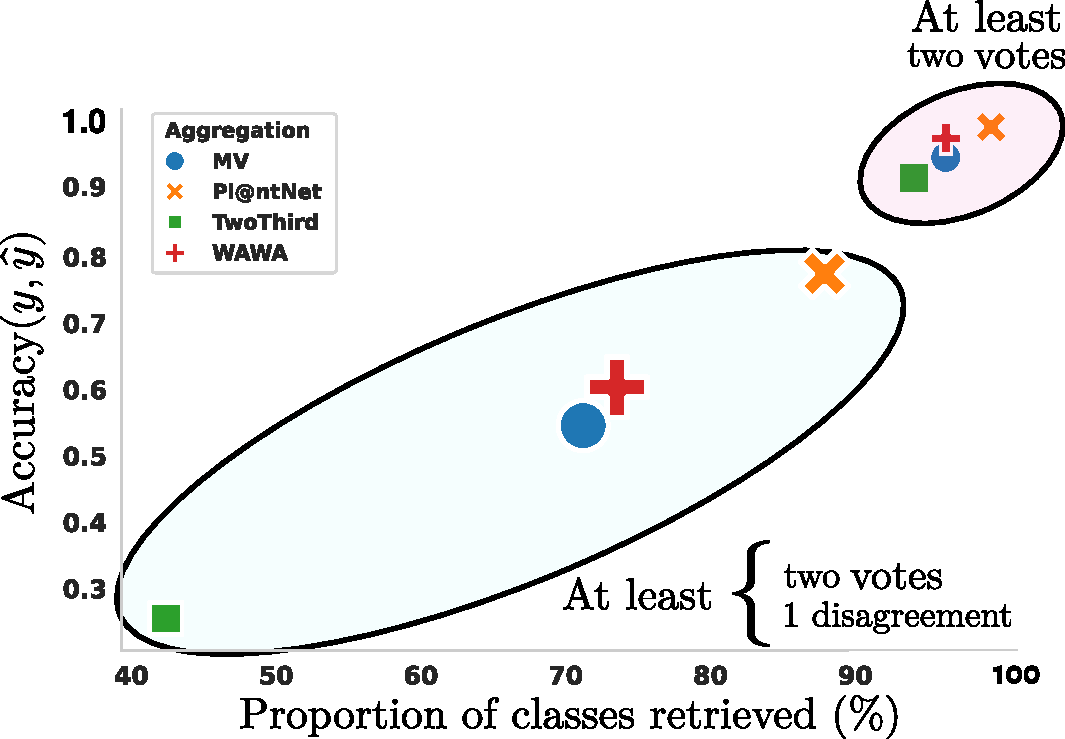
\includegraphics[width=\textwidth]{./images/both_accuracies.pdf}
\end{center}
%  \pause
%  \begin{block}{In short}
%    \begin{itemize}
%        \item Pl@ntNet aggregation performs better overall
%        \item TwoThird is highly impacted by their reject threshold
%        \item In ambiguous settings (right), strategies weighting users are better
%    \end{itemize}
%  \end{block}

\end{frame}
%%%%%%%%%%%%%%%%%%%%%%%%%%%%%%%%%%%%%%%%%%%%%%%%%%%%%%%%%%%%%%%%%%%%%%%%%%%%%%%

%%%%%%%%%%%%%%%%%%%%%%%%%%%%%%%%%%%%%%%%%%%%%%%%%%%%%%%%%%%%%%%%%%%%%%%%%%%%%%%
\begin{frame}{Integrating the AI vote}{}
\textbf{Why?}
\begin{itemize}
    \item More data
    \item Could correct non-xpert users
    \item Could invalidate bad quality observation
\end{itemize}
\pause
\vspace{2cm}
\textbf{Main danger}
\begin{itemize}
    \item Redundancy: users are already guided by AI predictions
\end{itemize}

\end{frame}
%%%%%%%%%%%%%%%%%%%%%%%%%%%%%%%%%%%%%%%%%%%%%%%%%%%%%%%%%%%%%%%%%%%%%%%%%%%%%%%

\begin{frame}{Strategies to integrate the AI vote}{}
\begin{itemize}
    \item AI \textbf{as worker}: naive integration
    \item AI \textbf{fixed weight}: weight=1.7 to invalidate two new users by $<\theta_{\text{conf}}$
    \item AI \textbf{invalidating}: fixed weight but can only invalidate observations
    \item AI \textbf{confident}: fixed weight on data with $\mathbb{P}(\text{predicted species}) > \theta_{\text{score}}$
\end{itemize}
\pause
\vspace{1cm}
\begin{center}
$\Longrightarrow$ \textcolor{red}{confident AI with $\theta_{\text{score}}=0.7$ performs best\dots \\ but invalidating AI could be preferred for safety} $\Longleftarrow$
\end{center}
\end{frame}
%%%%%%%%%%%%%%%%%%%%%%%%%%%%%%%%%%%%%%%%%%%%%%%%%%%%%%%%%%%%%%%%%%%%%%%%%%%%%%%
%%%%%%%%%%%%%%%%%%%%%%%%%%%%%%%%%%%%%%%%%%%%%%%%%%%%%%%%%%%%%%%%%%%%%%%%%%%%%%%

\section{Conclusion}

%%%%%%%%%%%%%%%%%%%%%%%%%%%%%%%%%%%%%%%%%%%%%%%%%%%%%%%%%%%%%%%%%%%%%%%%%%%%%%%
\begin{frame}{Conclusion and perspectives}{Key points}
\textbf{In short:}
\begin{itemize}
    \item \textbf{Identifying ambiguous data} in crowdsourced datasets
    \item Creation of the \textbf{\texttt{peerannot} library} to run reproducible experiments
    \item Release a \textbf{new large scale dataset}
    \item \textbf{Evaluation} and \textbf{improvements} of the Pl@ntNet crowdsourcing setting
\end{itemize}
    \pause
    \vspace{1cm}
\textbf{Perspectives:}
    \begin{itemize}
        \item Need for better data collection: \textbf{recommendation system}
        \item Extend the library for \textbf{multiclass} classification and \textbf{regression}
    \end{itemize}
    \pause
    \begin{flushright}
        Thank you!
    \end{flushright}
\end{frame}
%%%%%%%%%%%%%%%%%%%%%%%%%%%%%%%%%%%%%%%%%%%%%%%%%%%%%%%%%%%%%%%%%%%%%%%%%%%%%%%

\begin{frame}[allowframebreaks,noframenumbering]
    \frametitle{References}
    \footnotesize
    \printbibliography
\end{frame}
\end{document}